%
% HSR LaTex Template
% Copyright 2012, Florian Bentele
%
% Complete LaTex template for thesis at HSR, customized
% for Prof. Dr. Peter Heinzmann
%
% This document is free software: you can redistribute
% it and/or modify it under the terms of the GNU
% General Public License as published by the Free
% Software Foundation, either version 3 of the License,
% or (at your option) any later version.
%
% This document is distributed in the hope that it will
% be useful, but WITHOUT ANY WARRANTY; without even the
% implied warranty of MERCHANTABILITY or FITNESS FOR A
% PARTICULAR PURPOSE. See the GNU General Public
% License for more details.
%
% You should have received a copy of the GNU General
% Public License along with this document. If not, see
% <http://www.gnu.org/licenses/>.
%
\documentclass[12pt]{hsrthesis}

\makeindex

% add new glossaryentries here...
% use in tex with \gls{label}

\newglossaryentry{sqlite}{
	name=SQLite,
	description={SQLite ist eine Datenbankengine, welche ohne Konfiguration auskommt. Es handelt sich dabei um eine Datenbank in einer Datei},
	first={SQLite}
}

\newglossaryentry{http}{
	name=HTTP,
	description={Hypertext Transfer Protocol},
	first={Hypertext Transfer Protocol (HTTP)}
}

\newglossaryentry{php}{
	name=PHP,
	description={ PHP (Hypertext Preprocessor) ist eine Webprogrammiersprache, welche auf dem Server ausgeführt wird und in der Regel eine dynamische HTML Webseite generiert
	},
	first={PHP}
}

\newglossaryentry{json}{
	name=JSON,
	description={ JSON (JavaScript Opject Notation) ist eine Darstellungsform eines Objektes welches menschliche Lesbarkeit und maschinelle Verarbeitung zulässt},
	first={JavaScript Object Notation (JSON)}
}

\newglossaryentry{mariadb}{
	name=MariaDB,
	description={ MariaDB ist eine Weiterentwicklung der berühmten MySQL Datenbank. Sie ist Quelloffen und verfügt über hohe Kompatibilität zu MySQL. Für weitere Informationen sei auf den ausführlichen Artikel auf Wikipedia verwiesen:  \url{http://en.wikipedia.org/wiki/Mariadb}, aufgerufen am 07.05.2013
	},
	first={MariaDB}
}

\newglossaryentry{webframework}{
	name=Webframework,
	description={ Ein Webframework ist eine Entwicklungsbasis für die Softwareentwicklung von Webapplikationen, also serverbasierten Applikationen, welche über Webbbrowser aufgerufen werden. Das Framework übernimmt dabei grundlegende Funktionen und beschleunigt die Entwicklung.},
	first={Webframework}
}

\newglossaryentry{api}{
	name=API,
	description={ Die API (Application Programming Interface), beschreibt die Schnittstelle zu einem System oder einer Technologie},
	first={API}
}

\newglossaryentry{git}{
	name=git,
	description={ Das Versionscontrollsystem git ist ein dezentrales OpenSource Sourcecodeversionierungssystem, welches sich für die Entwicklung von Software in Teams sehr gut eignet},
	first={git}
}

\newglossaryentry{rwd}{
	name=Responsive Web Design,
	description={ Responsive Web Design beschreibt den Ansatz an das Endgerät anpassungsfähiger Webseiten. Eine Webseite, welche die Regeln des Responsive Web Designs einhält, wird auf allen möglichen Endgeräten, egal ob Smartphone, Tablet oder Notebook korrekt dargestellt}
}

\newglossaryentry{csv}{
	name=CSV,
	description={ Comma Separated Values, eine Tabellendarstellungsform und maschinenlesbares Format zur Darstellung von Daten},
	first={CSV (Comma Separated Values)}
}

\newglossaryentry{CRUD}{
	name=CRUD,
	description={ Das Akronym CRUD umfasst die grundlegenden Datenbankoperationen Create (Datensatz anlegen), Read (Datensatz lesen), Update (Datensatz aktualisieren) und Delete (Datensatz löschen).	}
}

\newglossaryentry{jsp}{
	name=JSP,
	description={ Die JavaServer Pages stellen dynamische Daten eines Servers in Form einer HTML Seite dar.},
	first={JSP (JavaServer Pages)}
}

\newglossaryentry{rup}{
	name=RUP,
	description={ Der Rational Unified Process (RUP) ist ein Vorgehensmodell zur Softwareentwicklung. RUP benutzt die Unified Modeling Language (UML) als Notationssprache.},
	first={RUP (Rational Unified Process)}
}

\makeglossaries

\begin{document}

% Title
%%%%%%%
\newcommand{\thesistitle}{TourLive Server- und Aufnahmesystem}
\newcommand{\thesisauthora}{Patrizia Heer}
\newcommand{\thesisauthorb}{Simon Stäheli}
\newcommand{\thesisauthorc}{Florian Bentele}
\newcommand{\professor}{Prof. Dr. Peter Heinzmann}
\newcommand{\thesistype}{Bachelorarbeit}
\newcommand{\departement}{Abteilung Informatik}
\newcommand{\school}{Hochschule für Technik Rapperswil}
\newcommand{\term}{Frühlingssemester 2013}
\newcommand{\thedate}{14. Juni 2013}
\newcommand{\timeperiode}{31.01.2013 - 14.06.2013}
\newcommand{\partner}{Lukas Frey, cnlab AG}
\newcommand{\expert}{Dr. Th. Siegenthaler, CSI Consulting AG}
\newcommand{\coreader}{Prof. Hansjörg Huser}
\newcommand{\workload}{1080 Stunden, 360h bzw. 12 ECTS pro Student}
\newcommand{\linktothesis}{https://tourlive.ch}

\setlength{\oddsidemargin}{20mm}
\maketitle
\setlength{\oddsidemargin}{20mm}

% Preface
%%%%%%%%%
\clearpage\mbox{}\clearpage
    
\chapter*{Abstract}
Das bestehende cnlab TourLive System, kurz TourLive, ermöglicht die Aufzeichnung von Positions-, Bild- und Videodaten an Radrennsportanlässen mittels Nokia Symbian Geräten. Die gesammelten Daten werden mittels Webservice an den TourLive Server übertragen und dort Radsportinteressierten präsentiert.

%Um den aktuellen Stand von Radrennen zu erfassen und diese Daten zu veröffentlichen, konnte bisher das TourLive System von der cnlab AG eingesetzt werden.

%Nokia Handys wurden in Begleitfahrzeugen an der Frontscheibe eingebaut und haben die aktuelle Position sowie Bilder aufgenommen. Diese Daten wurden dann an den TourLive Server geschickt, welcher die Informationen verarbeitet und als Webseite für Radsport interessierte präsentiert.

Im Rahmen dieser Bachelorarbeit wurde das über 10 jährige System analysiert, an die aktuellen Bedürfnisse angepasst sowie mit Hilfe moderner Technologien umgesetzt. Das TourLive System umfasst neu drei komplett voneinander getrennte Komponenten. Diese sind zum ersten die Aufnahmegeräte, welche durch moderne Android Smartphones ersetzt wurden, zum zweiten der eigentliche TourLive Server (Java Spring Webservice) und als drittes das Geräteverwaltungsportal (Java Spring Webservice). 


Die neue Komponente, das Geräteverwaltungsportal ermöglicht die vollumfängliche Fernverwaltung der Aufnahmesysteme, welche bisher nur in einem sehr rudimentären Rahmen möglich war. Neu ist auch die Art des Videostreams. Während bisher nur Einzelbilder übertragen wurden, die dann auf dem Server zu einem Videostream verarbeitet wurden, ermöglicht das neue System die Übertragung ganzer Videosequenzen die anschliessend aufeinanderfolgend abgespielt werden. Die Kommunikation zwischen den verschiedenen Komponenten erfolgt über eine moderne RESTful-JSON-Schnittstelle. 


Die Administrationsoberfläche des TourLive Servers ermöglicht eine konfortable Renn- und Etappenverwaltung und auch die  Aufwertung der grafischen Oberflächen kam nicht zu kurz. 


Das Endprodukt beinhaltet die vom Industriepartner gewünschte Funktionalität und einen Prototypen, welcher anhand eines Probelaufs erfolgreich getestet wurde. Die weitere Entwicklung und der allfällige Einsatz an Radrennen in der Schweiz liegt in den Händen des Industriepartners.

\chapter*{Aufgabenstellung}
\begin{tabular}{ll}
	Studiengang: & Informatik (I) \\
	Institut: & ITA: Internet-Technologien und Anwendungen \\
	Gruppe: & Patrizia Heer, Simon Stäheli, Florian Bentele \\
	Betreuer: & Prof. Dr. Peter Heinzmann  \\
	Koreferent: & Prof. H. Huser, HSR \\
	Experte: & Dr. Th. Siegenthaler, CSI Consulting AG  \\
	Industriepartner: & Swiss Cycling / cnlab software ag \\    
\end{tabular}\\

\section*{Ausgangslage}
Das cnlab TourLive-System\footnote{Tourlive-System, \url{www.tourlive.ch}, besucht am 30.04.2013} dient zur Renndatenerfassung an Sportanlässen. Es wird seit 2004 an der Tour de Suisse und bei den Rennsporttagen Gippingen eingesetzt. Die in Schiedsrichterfahrzeugen montierten mobilen Aufnahmesysteme (Nokia Mobiltelfonie mit Symbian-Anwendung) erfassen die Position von den Spitzenfahrern, den Verfolgern und dem Feld. Ferner liefern die Aufnahmesysteme Live-Bilder aus Sicht dieser Schiedsrichterfahrzeuge. Mit Hilfe der RadioTour-Android Tablet Anwendung notiert der RadioTour-Speaker die Zeitabstände und Zusammensetzung von Fahrergruppen. All diese Daten werden auf dem cnlab TourLive-Server gesammelt, aufbereitet und für die Publikation auf Webservern zu Verfügung gestellt. 
Swiss Cycling möchte die TourLive-Anwendung nun auch kleineren Rennveranstaltern zu Verfügung stellen können. In diesem Zusammenhang sollen auch die Aufnahmesysteme auf Android portiert und in der Funktionalität optimiert werden.
\section*{Ziel}
Das überarbeitete TourLive-System soll als Gesamtpaket für Rennveranstalter zu Verfügung gestellt werden können. Die Rennveranstalter sollen ihre Anlässe zusammen mit den Renninformationen auf der Webanwendungen (Datenerfassungs- und Aufbereitungssystem) präsentieren können. Die Aufnahmesysteme sollen auf Android Mobiles funktionieren und sie sollen über eine Management Anwendung überwacht und konfiguriert werden können.
\section*{Teilaufgaben}
\begin{itemize}
	\item Analyse
	\begin{itemize}
		\item Detailliertes Studium des aktuellen TourLive-Systems (Symbian Aufnahmesysteme und Webanwendung)
		\item Studium verschiedener Websites zu Radrennen, Erstellung einer Übersicht und Beurteilung der verschiedenen Elemente auf solchen Webseiten
		\item Festlegung der Funktionen der Aufnahme- und Darstellungssysteme
	\end{itemize}
	\item Entwicklung Android Aufnahmesysteme
	\begin{itemize}
		\item Positions- und Bildaufnahmen
		\item Alarming-Funktionen
		\item Logging-Funktionen
		\item Kommunikation mit verschiedenen Datenservern
	\end{itemize}
	\item Entwicklung Webanwendung (Webserver für Radrennen bei welchen mit TourLive und RadioTour Renndaten aufgezeichnet und dargestellt werden)
	\begin{itemize}
		\item Funktionsblöcke (Zeitabstände, Fahrergruppen, Bilder, LiveTicker, Kartendarstellung, Höhenprofil, Ranglisten, Marschtabellen, Fahrerinformationen, Abstände von Aufnahmesystemen, Distanz zum Werbe- und Renntross, Zeit bis dieser eine bestimmte Stelle passiert, …)
		\item Kommunikationsschnittstelle mit alten und neuen TourLive-Aufnahmesystemen
		\item Kommunikationsschnittstelle mit RadioTour-Anwendung
		\item Schnittstelle zu Zeiterfassungssystemen (Matsport)
		\item Rennadministration (Fahrerlisten)
	\end{itemize}
	\item Testeinsatz am 50. GP des Kantons Aargau vom Donnerstag, 6. Juni 2013 im Rahmen der Radsporttagen Gippingen 2013
\end{itemize}


\chapter*{Urheberschaft\footnote{Diese Erklärung basiert auf der Muster-Erklärung in den Richtlinien der HSR zur Durchführung
von Projekt-, Studien-, Diplom- oder Bachelorarbeiten \cite{hsrerklaerung}}}

\footnotetext{Diese Erklärung basiert auf der Muster-Erklärung in den Richtlinien der HSR zur Durchführung
von Projekt-, Studien-, Diplom- oder Bachelorarbeiten \cite{hsrerklaerung}}

Die vorliegende Arbeit basiert auf Ideen, Arbeitsleistungen, Hilfestellungen und Beiträgen gemäss folgender Aufstellung:

\begin{longtable}{p{4cm}|p{4cm}|p{4cm}}
\hline 
\textbf{Gegenstand, Leistung} & \textbf{Person} & \textbf{Funktion} \\ 
\hline 
\hline
TourLive Server & Florian Bentele & Programmierung \& Dokumentation \\ 
\hline 
Android Aufnahmesystem & Patrizia Heer \& Simon Stäheli & Programmierung \& Dokumentation \\ 
\hline 
Device Management Server & Patrizia Heer \& Simon Stäheli & Programmierung \& Dokumentation \\ 
\hline 
Lektorat & Ursina Bentele &  \\ 
\hline 
Lektorat & Doris Bentele &  \\ 
\hline 
Lektorat & Daniel Stucki &  \\ 
\hline 
Lektorat & Maura Weber &  \\ 
\hline
Design Poster & Rahel Naef &  \\ 
\hline  
Idee, Aufgabenstellung, Betreuung während der Arbeit & Prof. Dr. Peter Heinzmann & Verantwortlicher Professor \\
\hline
Betreuung \& zur Verfügungsstellung Infrastruktur & Lukas Frey & Industriepartner \\
\hline

\end{longtable} 

Wir erklären hiermit, 
\begin{itemize}
	\item dass wir die vorliegende Arbeit selber und ohne fremde Hilfe durchgeführt habe, ausser derjenigen, welche explizit in der Aufgabenstellung erwähnt ist oder mit dem Betreuer schriftlich vereinbart wurde,
	\item dass wir sämtliche verwendeten Quellen erwähnt und gemäss gängigen wissenschaftlichen Zitierregeln korrekt angegeben habe.
	\item das wir keine durch Copyright geschützten Materialien (z.B. Bilder) in dieser Arbeit in unerlaubter Weise genutzt habe. 
\end{itemize}

Rapperswil, \today

\vspace{10 mm}
\begin{tabular*}{\textwidth}{c @{\extracolsep{\fill}} cc}
\hline
Simon Stäheli & Florian Bentele & Patrizia Heer \\
\end{tabular*}

\chapter*{Vereinbarung zur weiteren Verwendung\footnote{Diese Vereinbarung basiert auf den Muster-Vereinbarungen in den Richtlinien der HSR zur Durchführung von Projekt-, Studien-, Diplom- oder Bachelorarbeiten vom 16. Februar 2009.} }

\section{Gegenstand der Vereinbarung}
Mit dieser Vereinbarung werden die Rechte über die Verwendung und die Weiterentwicklung der Ergebnisse der Bachelorarbeit TourLive vonSimon Stäheli, Florian Bentele und Patrizia Heer unter der Betreuung von Peter Heinzmann geregelt.

\section{Urheberrecht}
Die Urheberrechte stehen der Studentin / dem Student zu.

\section{Verwendung}
Die Ergebnisse der Arbeit dürfen sowohl von allen an der Arbeit beteiligten Parteien, d.h. von den Studenten, welche die Arbeit verfasst haben, vom verantwortlichen Professor sowie vom Industriepartner verwendet und weiter entwickelt werden. Die Namensnennung der beteiligten Parteien ist bei der Weiterverwendung erwünscht, aber nicht Pflicht.

\begin{tabular}{lr}
	Rapperswil, \today \\
	\vspace{10 mm} \\
	\hline 
	
	& Simon Stäheli \\
	Rapperswil, \today \\
	\vspace{10 mm} \\
	\hline 
	
	& Florian Bentele \\
	Rapperswil, \today \\
	\vspace{10 mm} \\
	\hline 
	
	& Patrizia Heer\\
	Rapperswil, \today \\
	\vspace{10 mm} \\
	\hline 
	
	& Prof. Dr. Peter Heinzmann \\
	Rapperswil, \today \\
	\vspace{10 mm} \\
	\hline 
	
	& Industriepartner, Lukas Frey, cnlab AG

\end{tabular}

\chapter*{Management Summary}
\section*{Ausgangslage}

Mit dem cnlab Tour Live System, nachfolgend TourLive genannt, werden an Radrennsportanlässen Live-Informationen (Positions-, Bild- und Videodaten) gesammelt, verarbeitet und in Form einer Webseite präsentiert. Das gegenwärtig eingesetzte System aus dem Jahr 2001  umfasst Nokia Symbian Aufnahmegeräte sowie einen PHP Webservice. TourLive wird an den verschiedensten Radrennsportanlässen in der Schweiz, unter anderem an der Tour de Suisse, eingesetzt. Partner und Auftraggeber dieses Projektes ist die TourLive-Entwicklerfirma cnlab Software AG. 
\\

In Zukunft soll TourLive auch für kleinere Radrennsportanlässe zu Verfügung gestellt werden können. Dazu wurde im Rahmen dieser Bachelorarbeit das TourLive System erneuert und erweitert. Neben den bestehenden Funktionalitäten soll im neuen  TourLive System – TourLive Next Generation - TourLiveNG - der Fokus auf die Fernverwaltung der Aufnahmegeräte gelegt werden. 
\\

Als Partner und Auftraggeber dieses Projektes tritt die cnlab Software AG auf, die das bestehende System in Zusammenarbeit mit dem Radsportverband Swisscycling betreibt.


\section*{Vorgehen}
Nach eingehender Analyse des bestehenden Systems wurden in Zusammenarbeit mit der cnlab Software AG die Anforderungen an TourLive NG spezifiziert. Als Basis diente die vorangegangene Analyse sowie die  Erfahrungswerte der cnlab Software AG aus den vergangenen Einsätzen. Mit Prototypen wurden einzelne Funktionen auf ihre Machbarkeit überprüft. Durch regelmässige Sitzungen mit der cnlab Software AG konnte spontan auf Änderungswünsche eingegangen. Als Projektvorgehensmodell wurde in groben Zügen der Rational Unified Process angewendet. 
\\

\section*{Ergebnisse}
Das neu entwickelte System TourLive next generation basiert auf drei Komponenten wie folgende Abbildung zeigt. 
\begin{figure}[H]
	\centering
	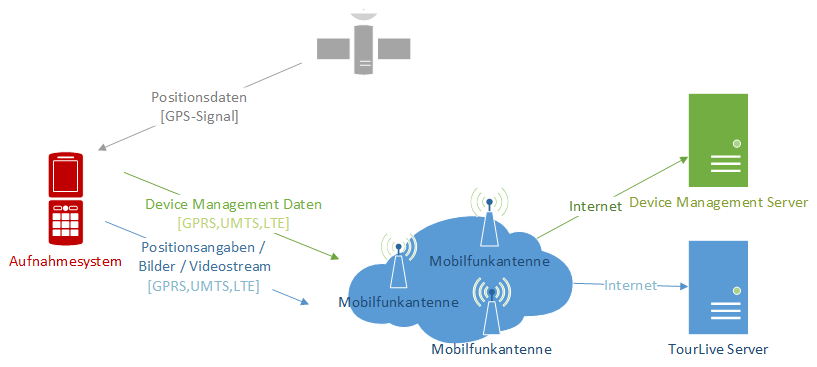
\includegraphics[width=150mm]{images/android/BigPicture_AndroidClient.png} 
	\caption{BigPicture TourLiveNG}
\end{figure}
Dies sind das auf Android basierende Aufnahmesystem, der TourLive Server und der Device Management Server. Der Geräteverwaltungsserver ermöglicht die Überwachung und Fernverwaltung der Aufnahmesysteme. Bei allfälligen Problemen ermöglicht ein Notfallwiederherstellungsdienst ein Neustart des Aufnahmesystems. Beide Serverkomponenten wurden mit dem Java Spring Framework realisiert. Sie verwenden zudem Twitter Bootstrap als GUI Framework und erfüllen damit unter Anwendung von \gls{rwd} die Anforderung einer dynamischen Webseite die auch auf Tablets und Smartphones korrekt angezeigt wird. 
\\

Rennen und Etappen können komfortabel über die Passwort gesicherte Administrationsoberfläche des TourLive Servers  verwaltet werden. Das Aufnahmesystem und die beiden Serverkomponenten kommunizieren über das Hypertext Transfer Protocol miteinander. Textdaten werden in einer JSON-Struktur übertragen während Video- und Bilddaten binär an den Server gesendet  werden. Der Videostream wird mit 10 sekündigen Videosequenzen realisiert die vom TourLive Server in ein vom Browser kompatibles Format konvertiert und mit Hilfes des HTML5 <video> Tags ausgeliefert werden. Aufgrund fehlender Standards und Browserinkompatibilitäten müssen die Videosequenzen in verschiedenen Videoformaten zur Verfügung gestellt werden.



\section*{Ausblick}
TourLiveNG wurde in der Schlussphase des Projektes an den Radsporttagen in Gippingen sowie an der ersten Etappe der Tour de Suisse ausgiebig getestet. Die Tests haben gezeigt, dass das System grundsätzlich eingesetzt werden kann. Es wurden aber auch noch die eine oder andere Optimierungsmöglichkeit eruriert. Eine wichtige Erkenntnis dieser Testläufe ist die Problematik mit der Wärmeentwicklung der Geräte bei direkter Sonneneinstrahlung. Ein paar kleine Optimierung konnten aufgrund dieser Tests noch vorgenommen werden. Diese und weitere, grössere Optimierungsmöglichkeiten wurden dokumentiert.
\\

Die Weiterentwicklung des Projektes liegt in den Händen der cnlab Software AG. Der Einsatz an weiteren Radrennen wird die cnlab Software AG gemeinsam mit dem Radsportverband Swisscycling prüfen.



% Table of contents
%%%%%%%%%%%%%%%%%%%
\setcounter{tocdepth}{1}
\tableofcontents

% Main content
%%%%%%%%%%%%%%%%%%
\chapter{Einleitung}

In der Einleitung werden die Systemkomponenten der Arbeit erläutert. Dadurch erhält man einen Überblick wie das Aufnahmesystem mit dem Server zusammenspielt. Für das Verständnis wird das Aufgabenumfeld in einem abstrakten Kontext dargestellt. Die konkrete Implementierung und detailierte Analyse werden dann in den folgenden Kapitel behandelt.

\section{Big Picture}
Zur Übersicht werden die verschiedenen Komponenten des Projektes in einem Big Picture zusammengefasst. Die Grafik \ref{fig:bigpicture} ist in drei Abschnitte unterteilt. Im obersten Abschnitt befinden sich alle Geräte, welche Daten erfassen. Diese Aufnahmesysteme bestehen aus der Android TourLiveApp, als Teil dieser Arbeit, sowie dem Android RadioTourSpeaker welcher im Rahmen einer anderen Arbeit entwickelt wurde.\\
Im mittleren Teil befinden sich die Serversysteme. Diese besteht aus einem TourLive Server, welcher die Renndaten empfängt und verarbeitet sowie dem Geräteverwaltungsserver. Der Geräteverwaltungsserver bietet eine Übersicht über die registrierten Aufnahmesysteme und ermöglicht es deren Einstellungen zu Verwalten sowie allfällige Fehlerquellen frühzeitig zu erkennen.\\
Der unterste Abschnitt zeigt die Anwendergruppen, die mit den Daten beliefert werden. Dies sind zum einen die Besucher der Webseite, welche in dieser Arbeit umgesetzt wurde, sowie auch Drittentwickler, die Interesse an diesen Daten haben.\\
Teil dieser Arbeit sind die farblich hervorgehobenen Komponenten: Die Aufnahmesysteme TourLiveApp in Form einer Android App [rot], das Serversystem TourLive Server in Form einer Spring Webapplikation [blau] sowie das Serversystem Device Management Server ebenfalls in Form einer Spring Webapplikation [grün].

\begin{figure}[H]
	\centering
	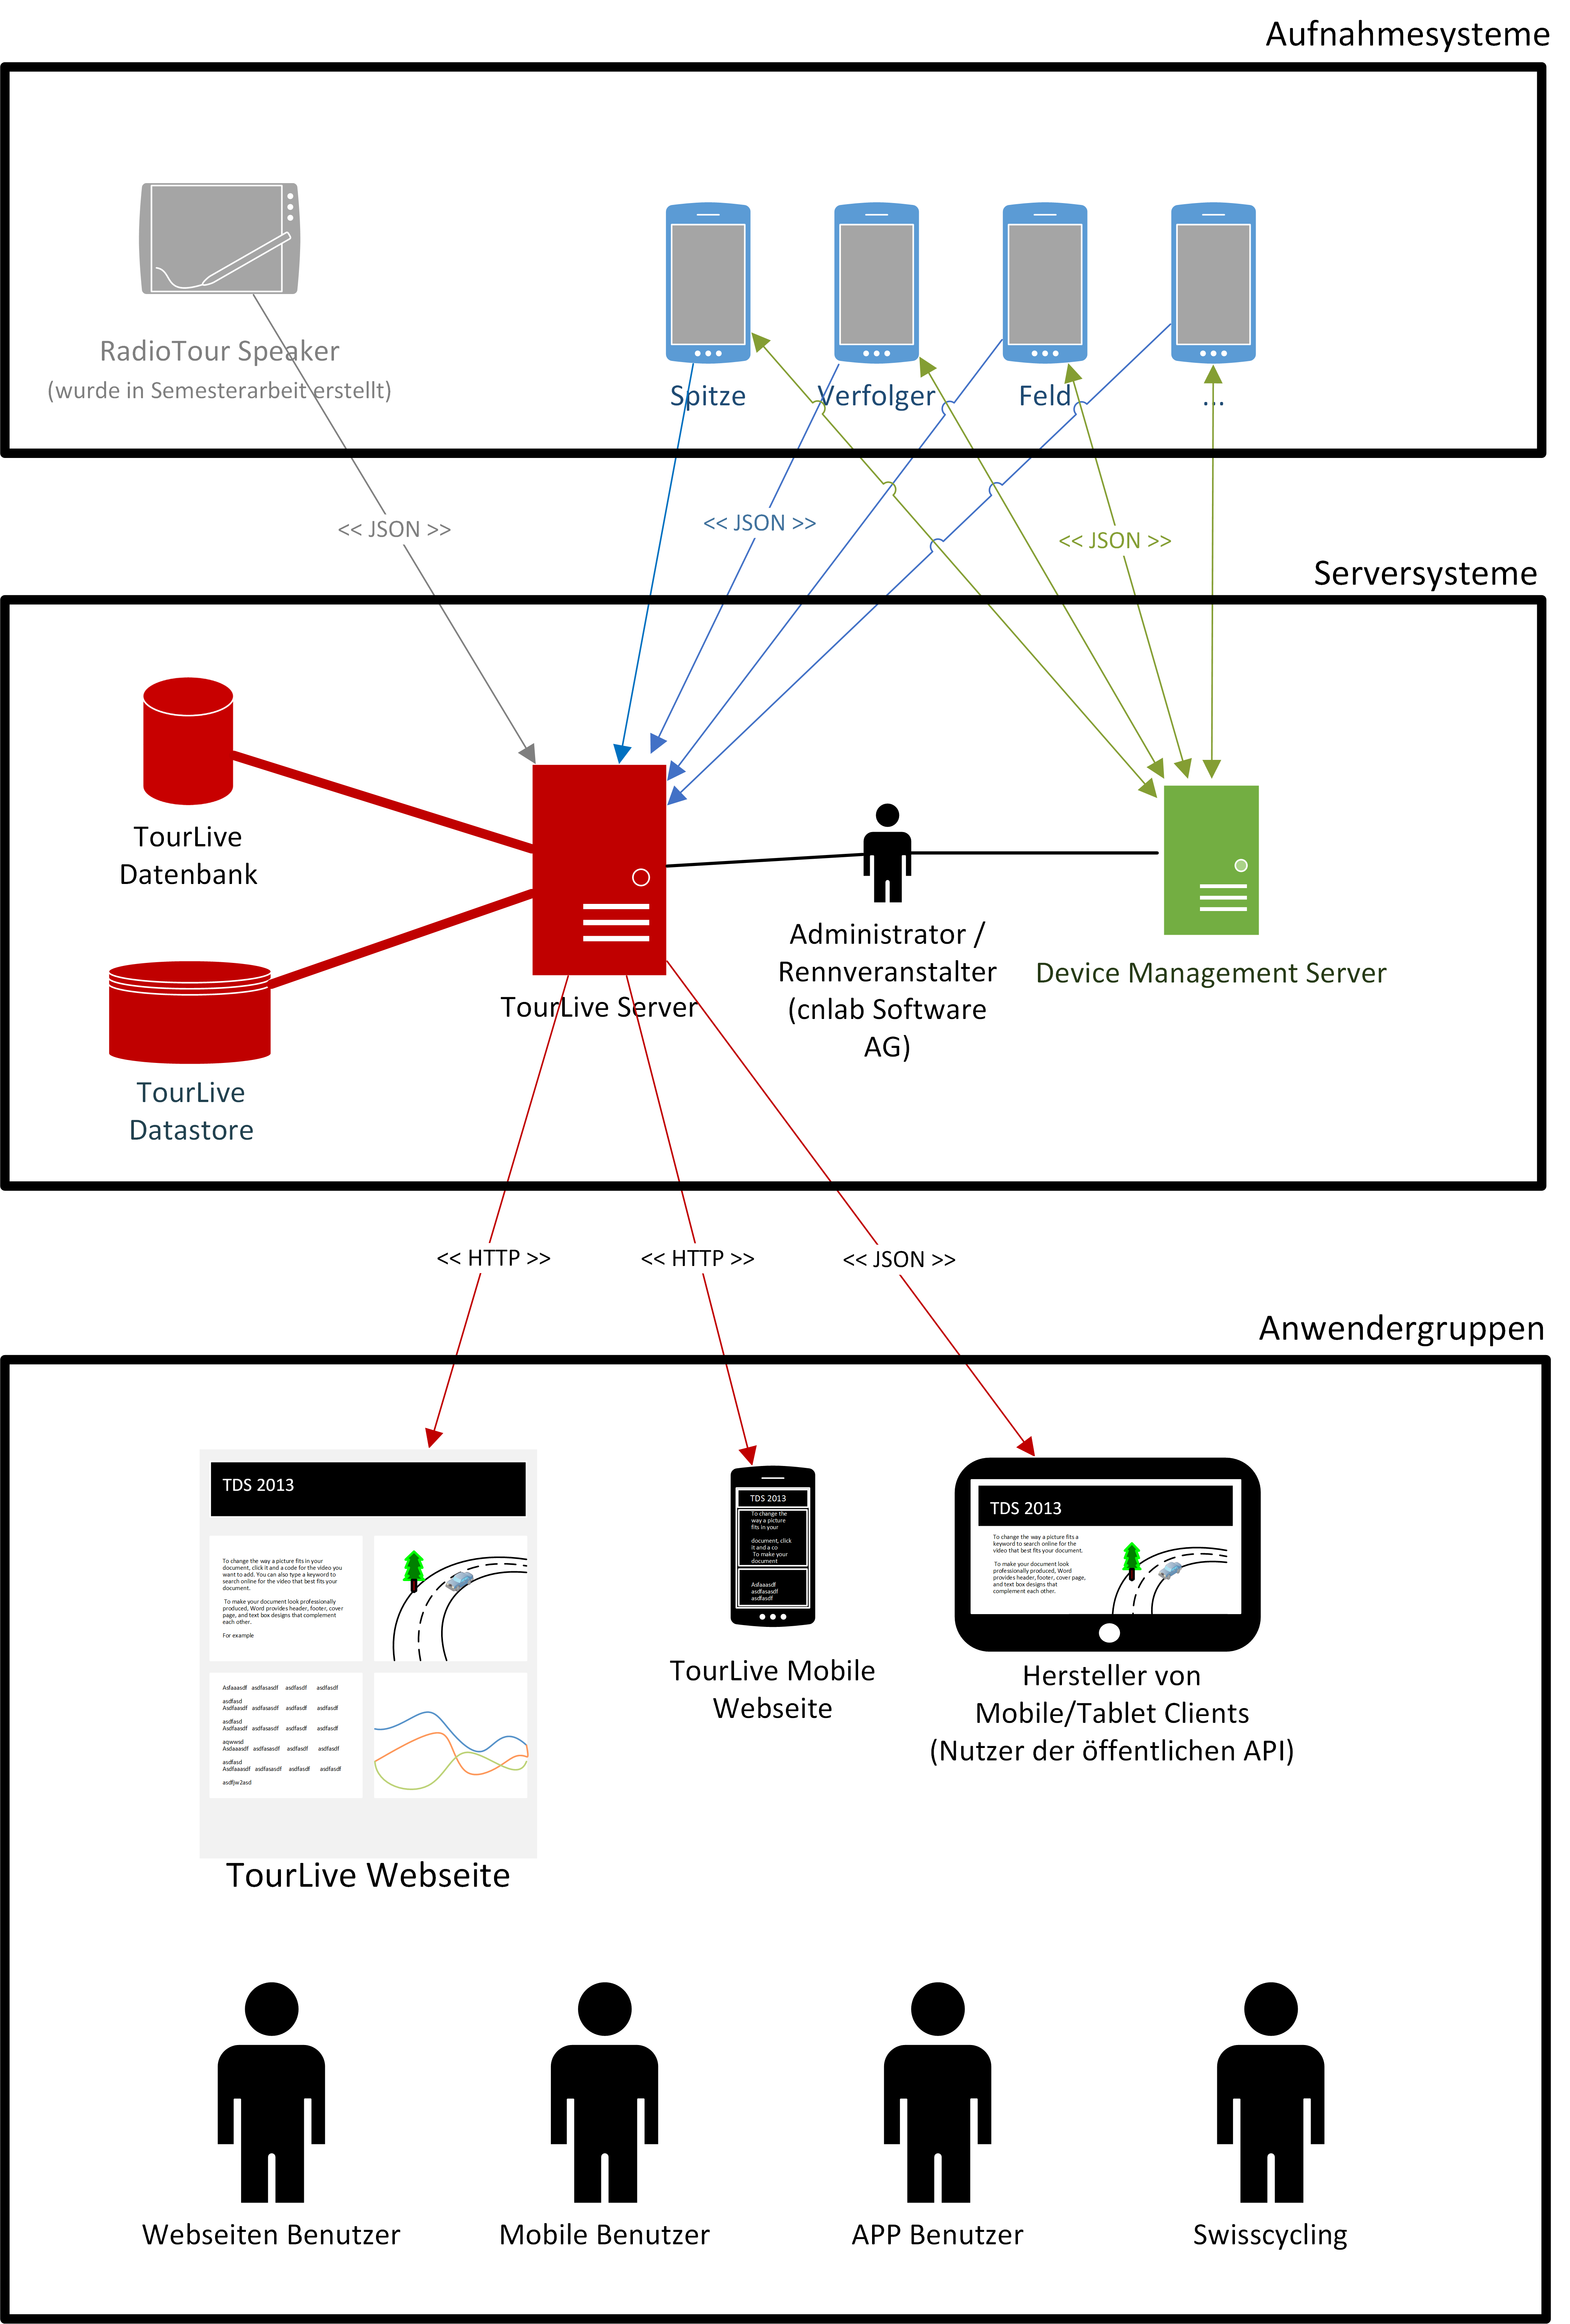
\includegraphics[height=200mm]{images/BigPicture.png}
	\caption{BigPicture}
	\label{fig:bigpicture}
\end{figure}

\pagebreak

\section{Kernelemente}
Die drei oben erwähnten Kernsysteme werden im folgenden kurz beschrieben.

\subsection{TourLive Server}
Auf der zentralen Webapplikation TourLive Server werden die eingehenden Daten von den Aufnahmesystemen gespeichert, verarbeitet, aufbereitet und weitergegeben. Bild und Positionsdaten werden in Form einer Webseite für Radsportbegeisterte aufbereitet und für mögliche Drittentwickler zur Verfügung gestellt. Die Architektur wurde dabei so gewählt, dass das System bei hoher Last gut skaliert. Diese Komponente wird im Kapitel \ref{sec:tourliveserver} genauer behandelt.

\subsection{Device Management Server}
Der Device Management Server hilft dabei, die aktiven Aufnahmegeräte zu verwalten. Es ersetzt das existierende Portal, dass nur wenig Funktionalität besitzt. Sollte der Device Management Server nicht verfügbar sein, sind die Aufnahmegeräte trotzdem einsatzfähig, da die Einstellungen lokal am Smartphone gesetzt werden können.

\subsection{Aufnahmesystem}
Ein wesentlicher Bestandteil des Endsystems ist das Aufnahmesystem. Es ersetzt die Symbian App auf den Nokia Handys. In der folgenden Abbildung sieht man links das Aufnahmesystem, welches von den Satelliten GPS Daten empfängt. Periodisch werden alle gesammelten Daten vom Aufnahmesystem an den TourLive Server übermittelt. Ebenfalls periodisch werden die Einstellungen vom Device Management Server abgeholt. Werden die Einstellungen lokal verändert so werden die veränderten Einstellungen an den Device Management Server übertragen.
\begin{figure}[H]
	\centering
	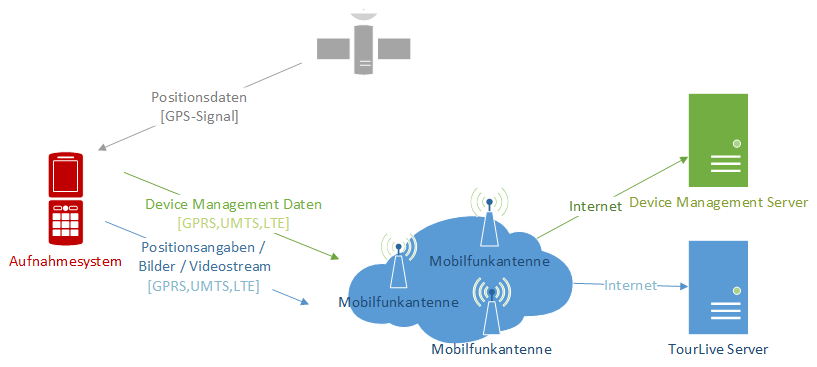
\includegraphics[width=150mm]{images/android/BigPicture_AndroidClient.png} 
	\caption{BigPicture Android Aufnahmesystem}
\end{figure}

\section{Aufgabenaufteilung}
{\renewcommand{\arraystretch}{2}%
    \begin{longtable}{  p{7.0cm} | p{4.0cm} }
    \textbf{Komponente} & \textbf{Bearbeitet durch} \\ 
  	\hline
	\hline
    TourLive Server & Florian Bentele \\
    \hline
    TourLiveApp & Patrizia Heer\newline Simon Stäheli \\
    \hline
    Device Management Server & Patrizia Heer \newline Simon Stäheli \\
    \hline
\caption{Aufgabenaufteilung}
\end{longtable}}

\chapter{TourLive Server}
\label{sec:tourliveserver}
In den folgenden Abschnitten wird die Webapplikation TourLive Server erläutert. Dabei liegt der Fokus auf der Spezifikation und deren technischen Umsetzung. Dieses Kapitel richtet sich ins Besondere an Entwickler, welche an diesem Projekt weiterarbeiten möchten und an Personen, welche an den technischen Details interessiert sind.

\section{Software Analyse}
\subsection{Spezifikation}
Weite Teile der Anforderungen an die Webapplikation ergeben sich aus der Analyse der bestehenden Lösung. Im Einsatz ist zur Zeit eine, von der cnlab AG entwickelte \textit{\gls{php}} Webapplikation. Grundsätzlich soll die Funktionalität der bestehenden Lösung erweitert und in technologischer Sicht auf den aktuellsten Stand gebracht werden. In der folgenden Tabelle \ref{tab:tourlivewebspeztable} ist jeweils zu erkennen, ob es sich um eine neue Funktion handelt oder eine Bestehende erweitert wurde.
\\

Die Analyse der funktionalen Anforderungen und Usecases sind im Anhang \ref{sec:tourliveusecase} umfangreich Dokumentiert.

\begin{longtable}{ p{3.5cm} | p{4.3cm} | p{4.3cm} }
	\textbf{Spezifikation} & \textbf{Altes System} & \textbf{Neues System} \\ \hline\hline Renn- und Etappenverwaltung & - & Benutzerfreundliche Renn- und Etappenverwaltung\\ \hline
Bildübertragung & 1 Bild / Zeitpunkt (auch bei mehreren Aufnahmegeräten) & Konfigurierbare Bildübertragung\\ \hline
Streckenprofil & Aktuelle Position & Alle Positionen (HTML5, SVG\footnote{HTML5 und SVG sind zwei moderne Webtechnologien um grafiken im Browser zu zeichnen})\\ \hline
Zeitliche Abstände & Distanz in Zeit und km zwischen Geräten & Rückstand relativ zur Spitze in Zeit und km, sowie Durchschnittsgeschwindigkeit und Höhenmeter\\ \hline
Rennsituation & Fahrer werden gruppiert dargestellt & Fahrer mit weiteren Informationen angereichert\\ \hline
Rangliste & - & Aktuelle (virtuelle) Rangliste, sortierbar\\ \hline
Marschtabelle & - & Marschtabelle mit Informationen und allen Positionen der Aufnahmegeräten\\ \hline
Kartenausschnitt & Position der Aufnahmesysteme & Poistionen der Aufnahmesysteme (Farbe wählbar)\\ \hline
Replay & Vergangene Rennen abspielbar & Rennen vor und zurück spulen nach Zeit und Renn Km\\ \hline
Werbebanner & Statische Werbung & Einbetten von HTML Code für Werbeblock\\ \hline
Mobile Client & - & Webseite optimiert für alle Bildschirmgrössen und Geräte\\ \hline

\caption{Spezifikation TourLive Server}
\label{tab:tourlivewebspeztable}
\end{longtable}

\subsection{Evaluation Webframework}
\label{sec:tourliveserverevaluationwebframework}
Wie aus der Aufgabenstellung zu entnehmen ist, wird keine spezifische Technologie für die Umsetzung des TourLive Server festgelegt. Vielmehr ist es Teil der Arbeit eine geeignete Lösung zu evaluieren und dabei auf ein \textit{\gls{webframework}} zurückzugreifen.\\
Die Anforderungen an das neue TourLive System bilden die Basis für die Evaluation eines dafür geeigneten Webframeworks.
\\
In einem nächsten Schritt wurden mögliche Lösungen gesucht und auf die obigen Anforderungen geprüft. Aktuell beliebte und verbreitete Frameworks wie Django (basierend auf der Programmiersprache Python) oder Ruby on Rails seinen an dieser Stelle als Beispiele erwähnt. Für die detaillierte Evaluation und Gewichtung der Kriterien wird aber auf Kapitel \ref{sec:evaluationwebframework} im Anhang verwiesen.

\subsubsection{Entscheid}
Zusammen mit dem Industriepartner fällt die Entscheidung auf das Java basierte Spring MVC Framework\footnote{Java Spring Framework Family, \url{http://springsource.org}, aufgerufen am 16.052013)}. Da die Frameworks sehr ähnliche Ideen verfolgen und sich daher, abstrakt betrachtet, kaum unterscheiden. Ausschlaggebend für diesen Entscheid waren schlussendlich die Vorkenntnisse der Studenten in der Java Technologie. 

\subsection{Weitere Technologien}
Die folgenden weiteren Technologien wurden für die Umsetzung des TourLive Server verwendet. Im Kapitel \ref{sec:wekzeugeundentwicklungsumgebung} im Anhang sind spezifische Tools und Entwicklungsumgebungen für die weitere Entwicklung aufgeführt.

\subsubsection{ORM und Datenbank}
Für die Persistierung sämtlicher Daten wird die MySQL ähnliche, quelloffene Datenbank MariaDB\footnote{MariaDB, \url{https://mariadb.org/}, aufgerufen am 16.05.2013} verwendet. Dies ist eine Anforderung des Industriepartners cnlab AG.
\\

Die Abbildung des Models auf der Datenbank übernimmt das Java ORM Framework Hibernate\footnote{Hibernate ORM, \url{http://www.hibernate.org/}, aufgerufen am 16.05.2013}, dank unzähliger Datenbanktreiber kann ein beliebiges Datenbanksystem, unter anderem auch MariaDB, verwendet werden.

\subsubsection{Maven}
Für die Verwaltung der externen Java Libraries wird Apache Maven\footnote{Apache Maven, \url{http://maven.apache.org/}, aufgerufen am 16.05.2013} verwendet. Maven lädt die definierten Abhängigkeiten automatisch und kompiliert das Projekt. Weiter generiert Maven die Javadoc\footnote{Javadoc, \url{http://de.wikipedia.org/wiki/Javadoc}, aufgerufen am 16.05.2013} Dokumentation zum Projekt und kann Auswertungen und statische Codeanalysen erzeugen.

\subsubsection{Twitter Bootstrap}
Die Daten werden mit dem Front-End Framework Twitter Bootstap in Form einer HTML Webseite dargestellt. Twitter Bootstrap vereinfacht und beschleunigt die Entwicklung von Webseiten indem es gewisse grundlegende Elemente anbietet. Es besteht aus einer komprimierten JavaScript und einer CSS Datei und kann durch viele Plugins erweitert oder verändert werden. Twitter Bootstrap ist OpenSource und in der Entwicklergemeinde sehr beliebt, da es unter anderem Webseiten für verschiedene Bildschirmgrössen (inkl. Smartphones und Tablets) optimal anpasst.

\subsection{Domain Model}
In der folgenden Abbildung \ref{fig:tourliveserverdomainmodel} wird die Problem Domain schematisch dargestellt. Die Renn- und insbesondere die Etappenklasse stehen im Zentrum der Abbildung, da die Informationen dort zusammengeführt werden. Die Umsetzung der einzelnen Elementen wird im nächsten Abschnitt \ref{sec:tourliveserversoftwaredesign} behandelt. 

\begin{figure}[H]
	\centering
	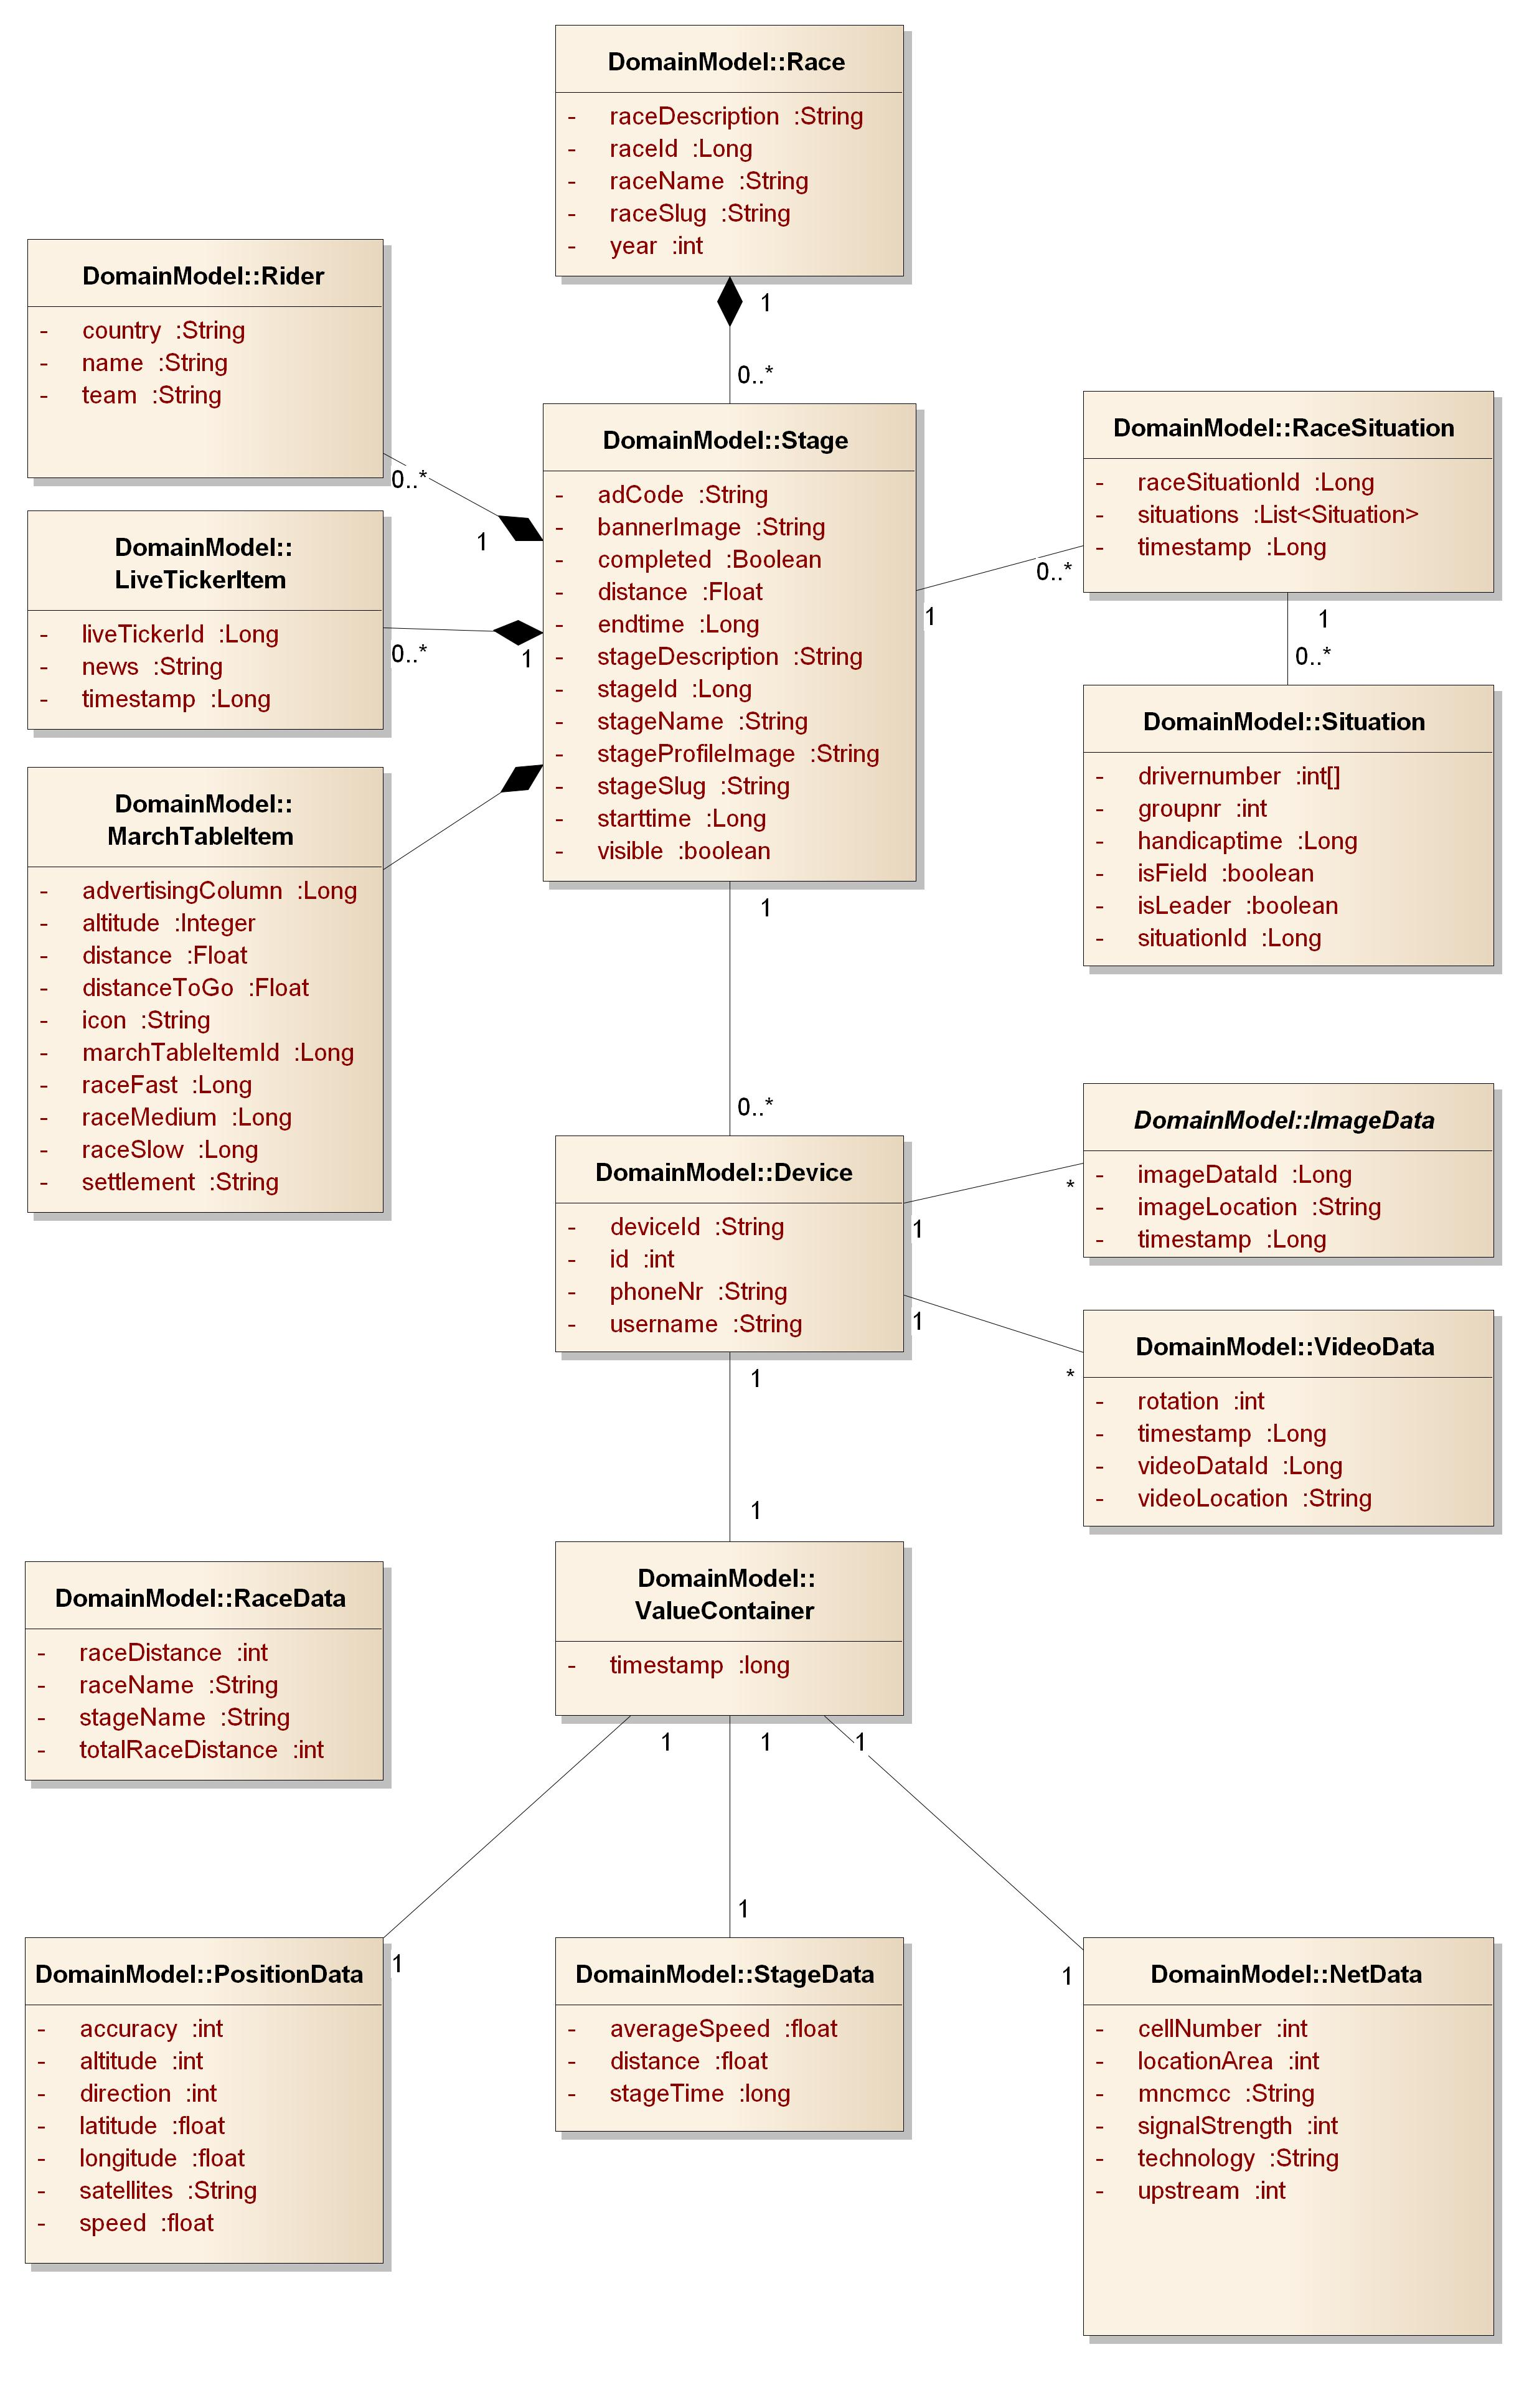
\includegraphics[width=130mm]{images/tourliveweb/TourLiveServer_DomainModel_ohneRand.jpg}
	\caption{Domain Model des TourLive Servers}
	\label{fig:tourliveserverdomainmodel}
\end{figure}

\section{Software Design}
\label{sec:tourliveserversoftwaredesign}
Dieser Abschnitt behandelt die Umsetzung der Spezifikationen zum Endzustand. Nach einer kurzen Architekturübersicht wird jede Teilkomponente einzeln erläutert.

\subsection{Architektur und Übersicht}
Der TourLive Server übernimmt zwei grundsätzlich Funktionen, zum einen die Präsentation der Daten und zum anderen die Schnittstelle (\textit{\gls{api}}) für die Aufnahmegeräte und Drittentwickler.
\begin{figure}[H]
	\centering
	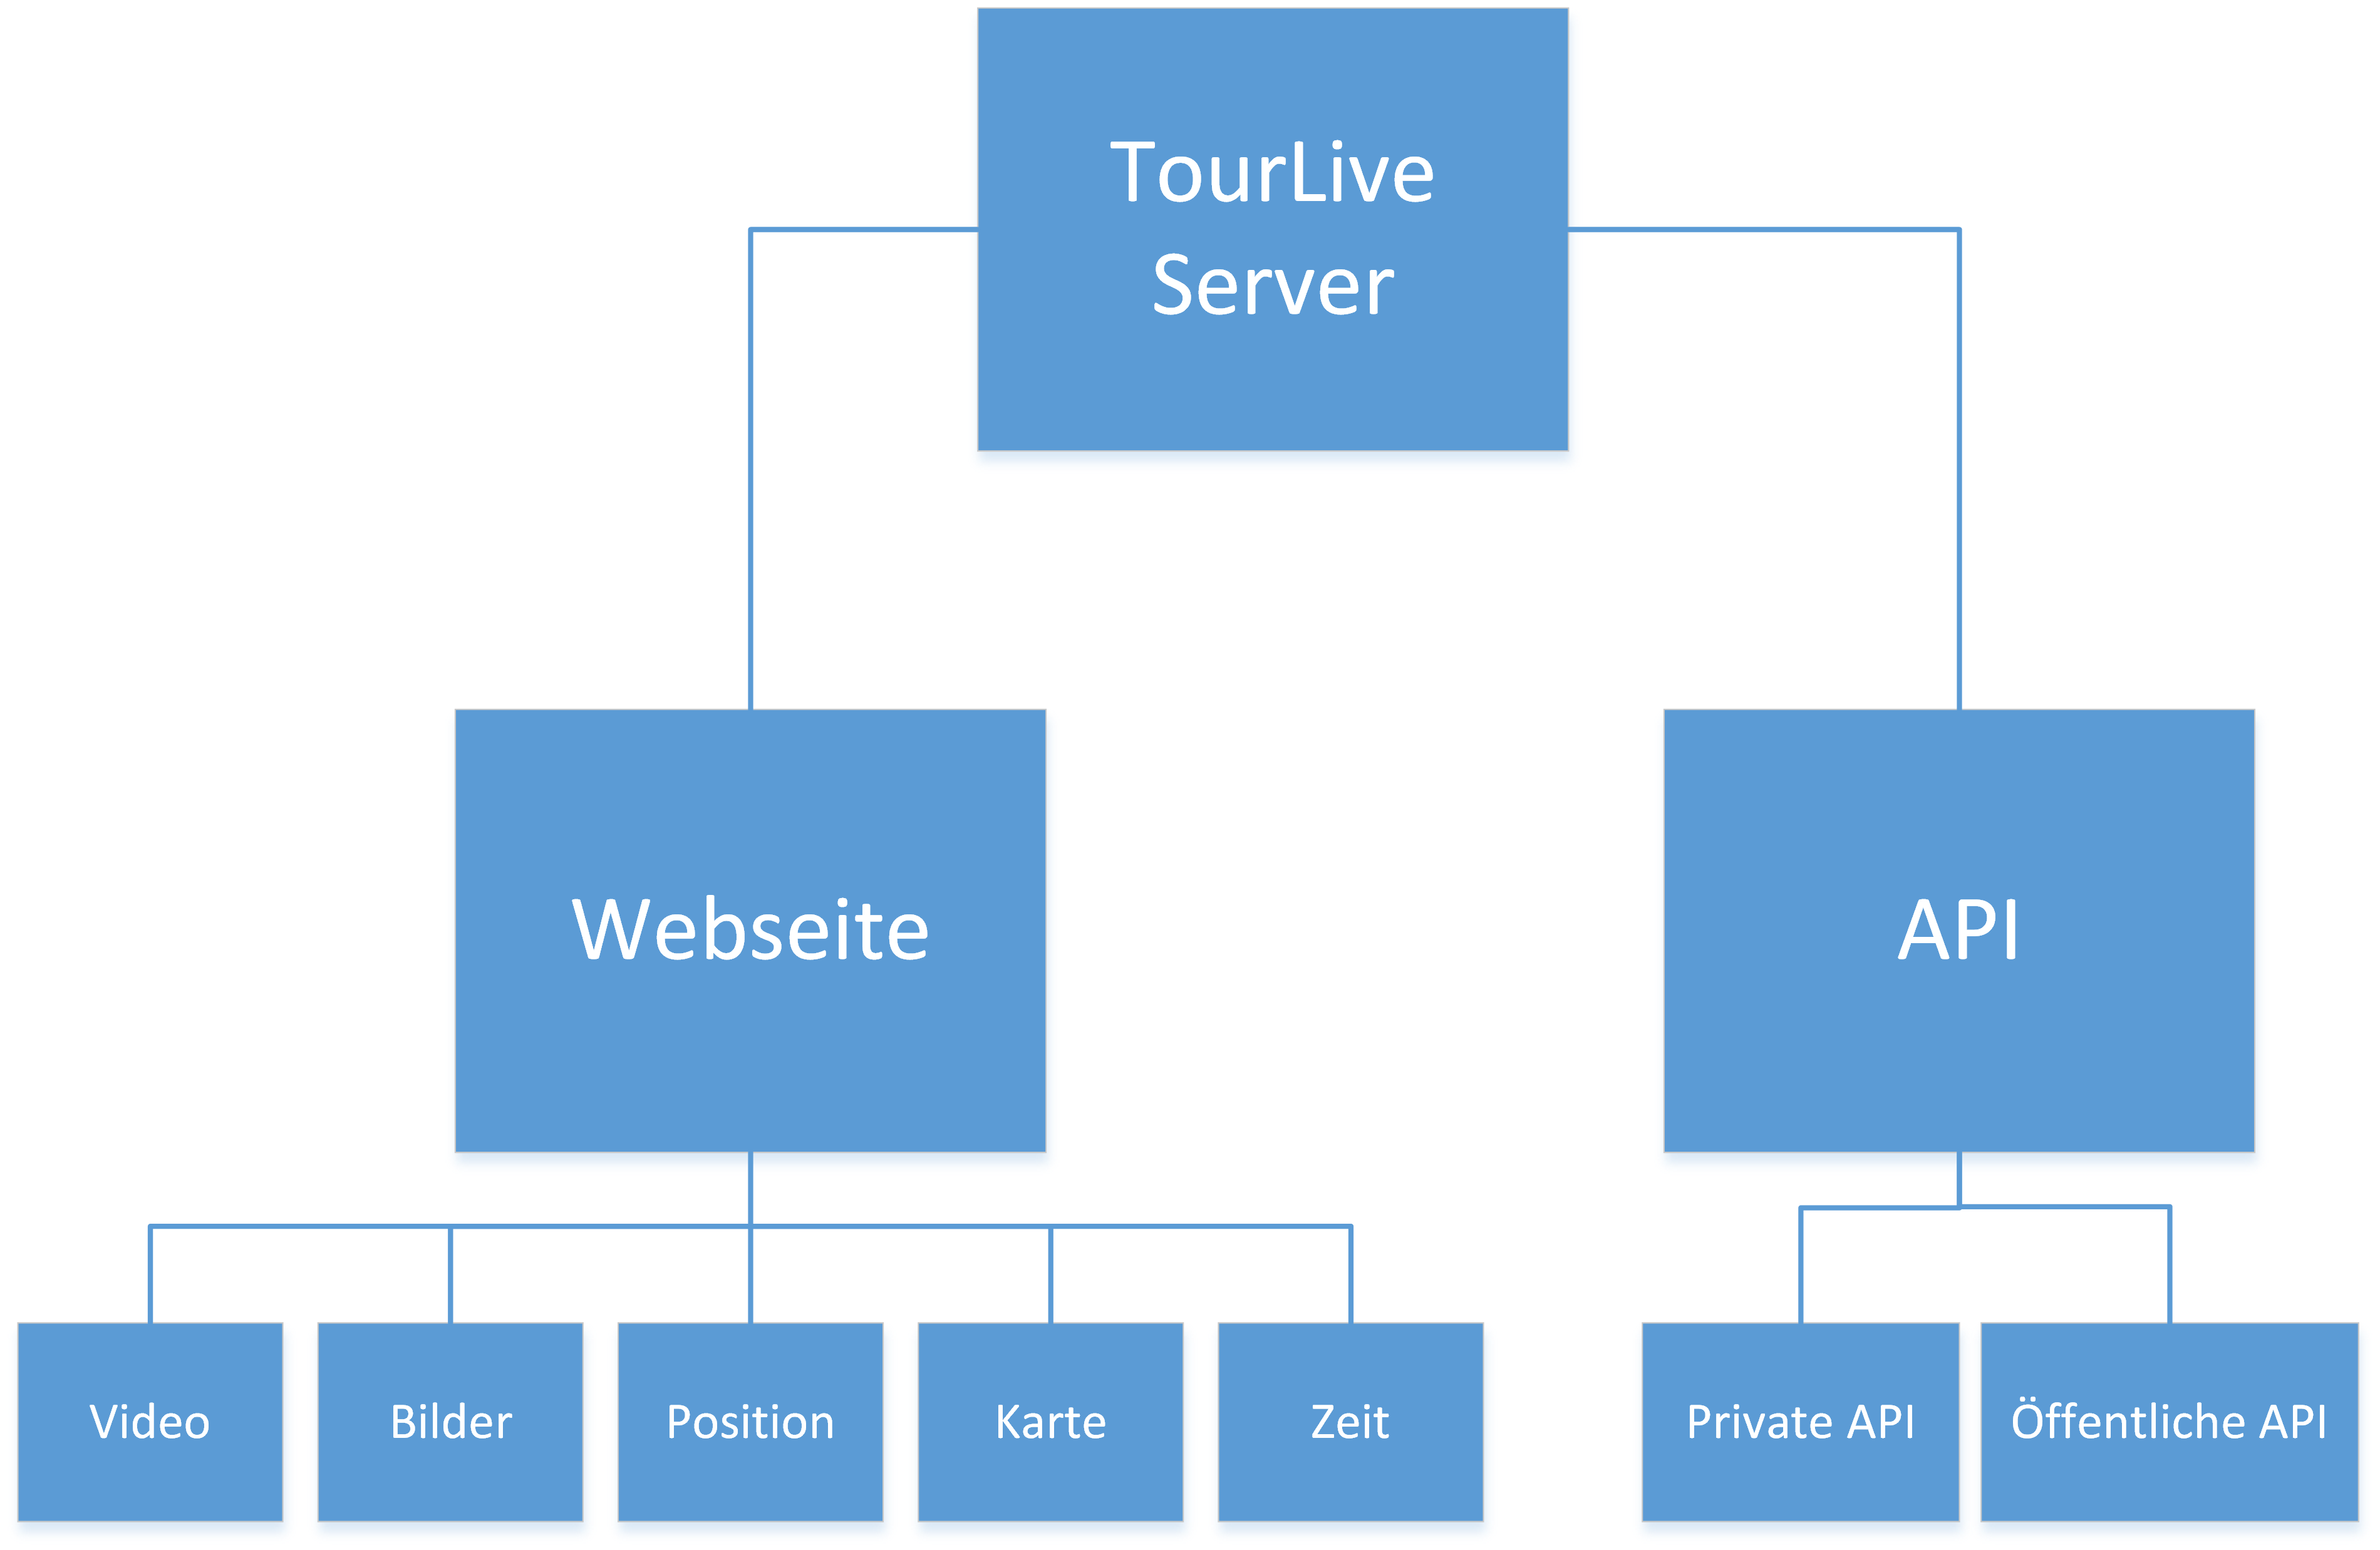
\includegraphics[width=130mm]{images/tourliveweb/uebersicht_tourlive.png}
	\caption{Grobstruktur des TourLive Servers}
	\label{fig:grobstrukturtourliveserver}
\end{figure}
Diese Aufteilung wurde ganz bewusst so gewählt, da es die Möglichkeit offen lässt, die Dienste auf mehrere Server aufzuteilen. Aus dem Requirements Engineering kam hervor, dass das System auch unter grosser Last für die Datenerfassung immer zur Verfügung stehen muss. In der Entwicklungsphase wurde darauf verzichtet das System auf mehrere Server aufzuteilen, da es das Testing erschwert.

\subsection{Schichtenmodell und Packagediagramm}
Ein Spring MVC Projekt legt eine gewisse Struktur vor, wie eine Webapplikation aufgebaut werden soll. Dadurch fördern Sie gute Programmierpraktiken und erzeugen gewisse Standards. Auch beim TourLive Server wurden diese Vorgaben angewendet.
\\

\begin{figure}[H]
	\centering
	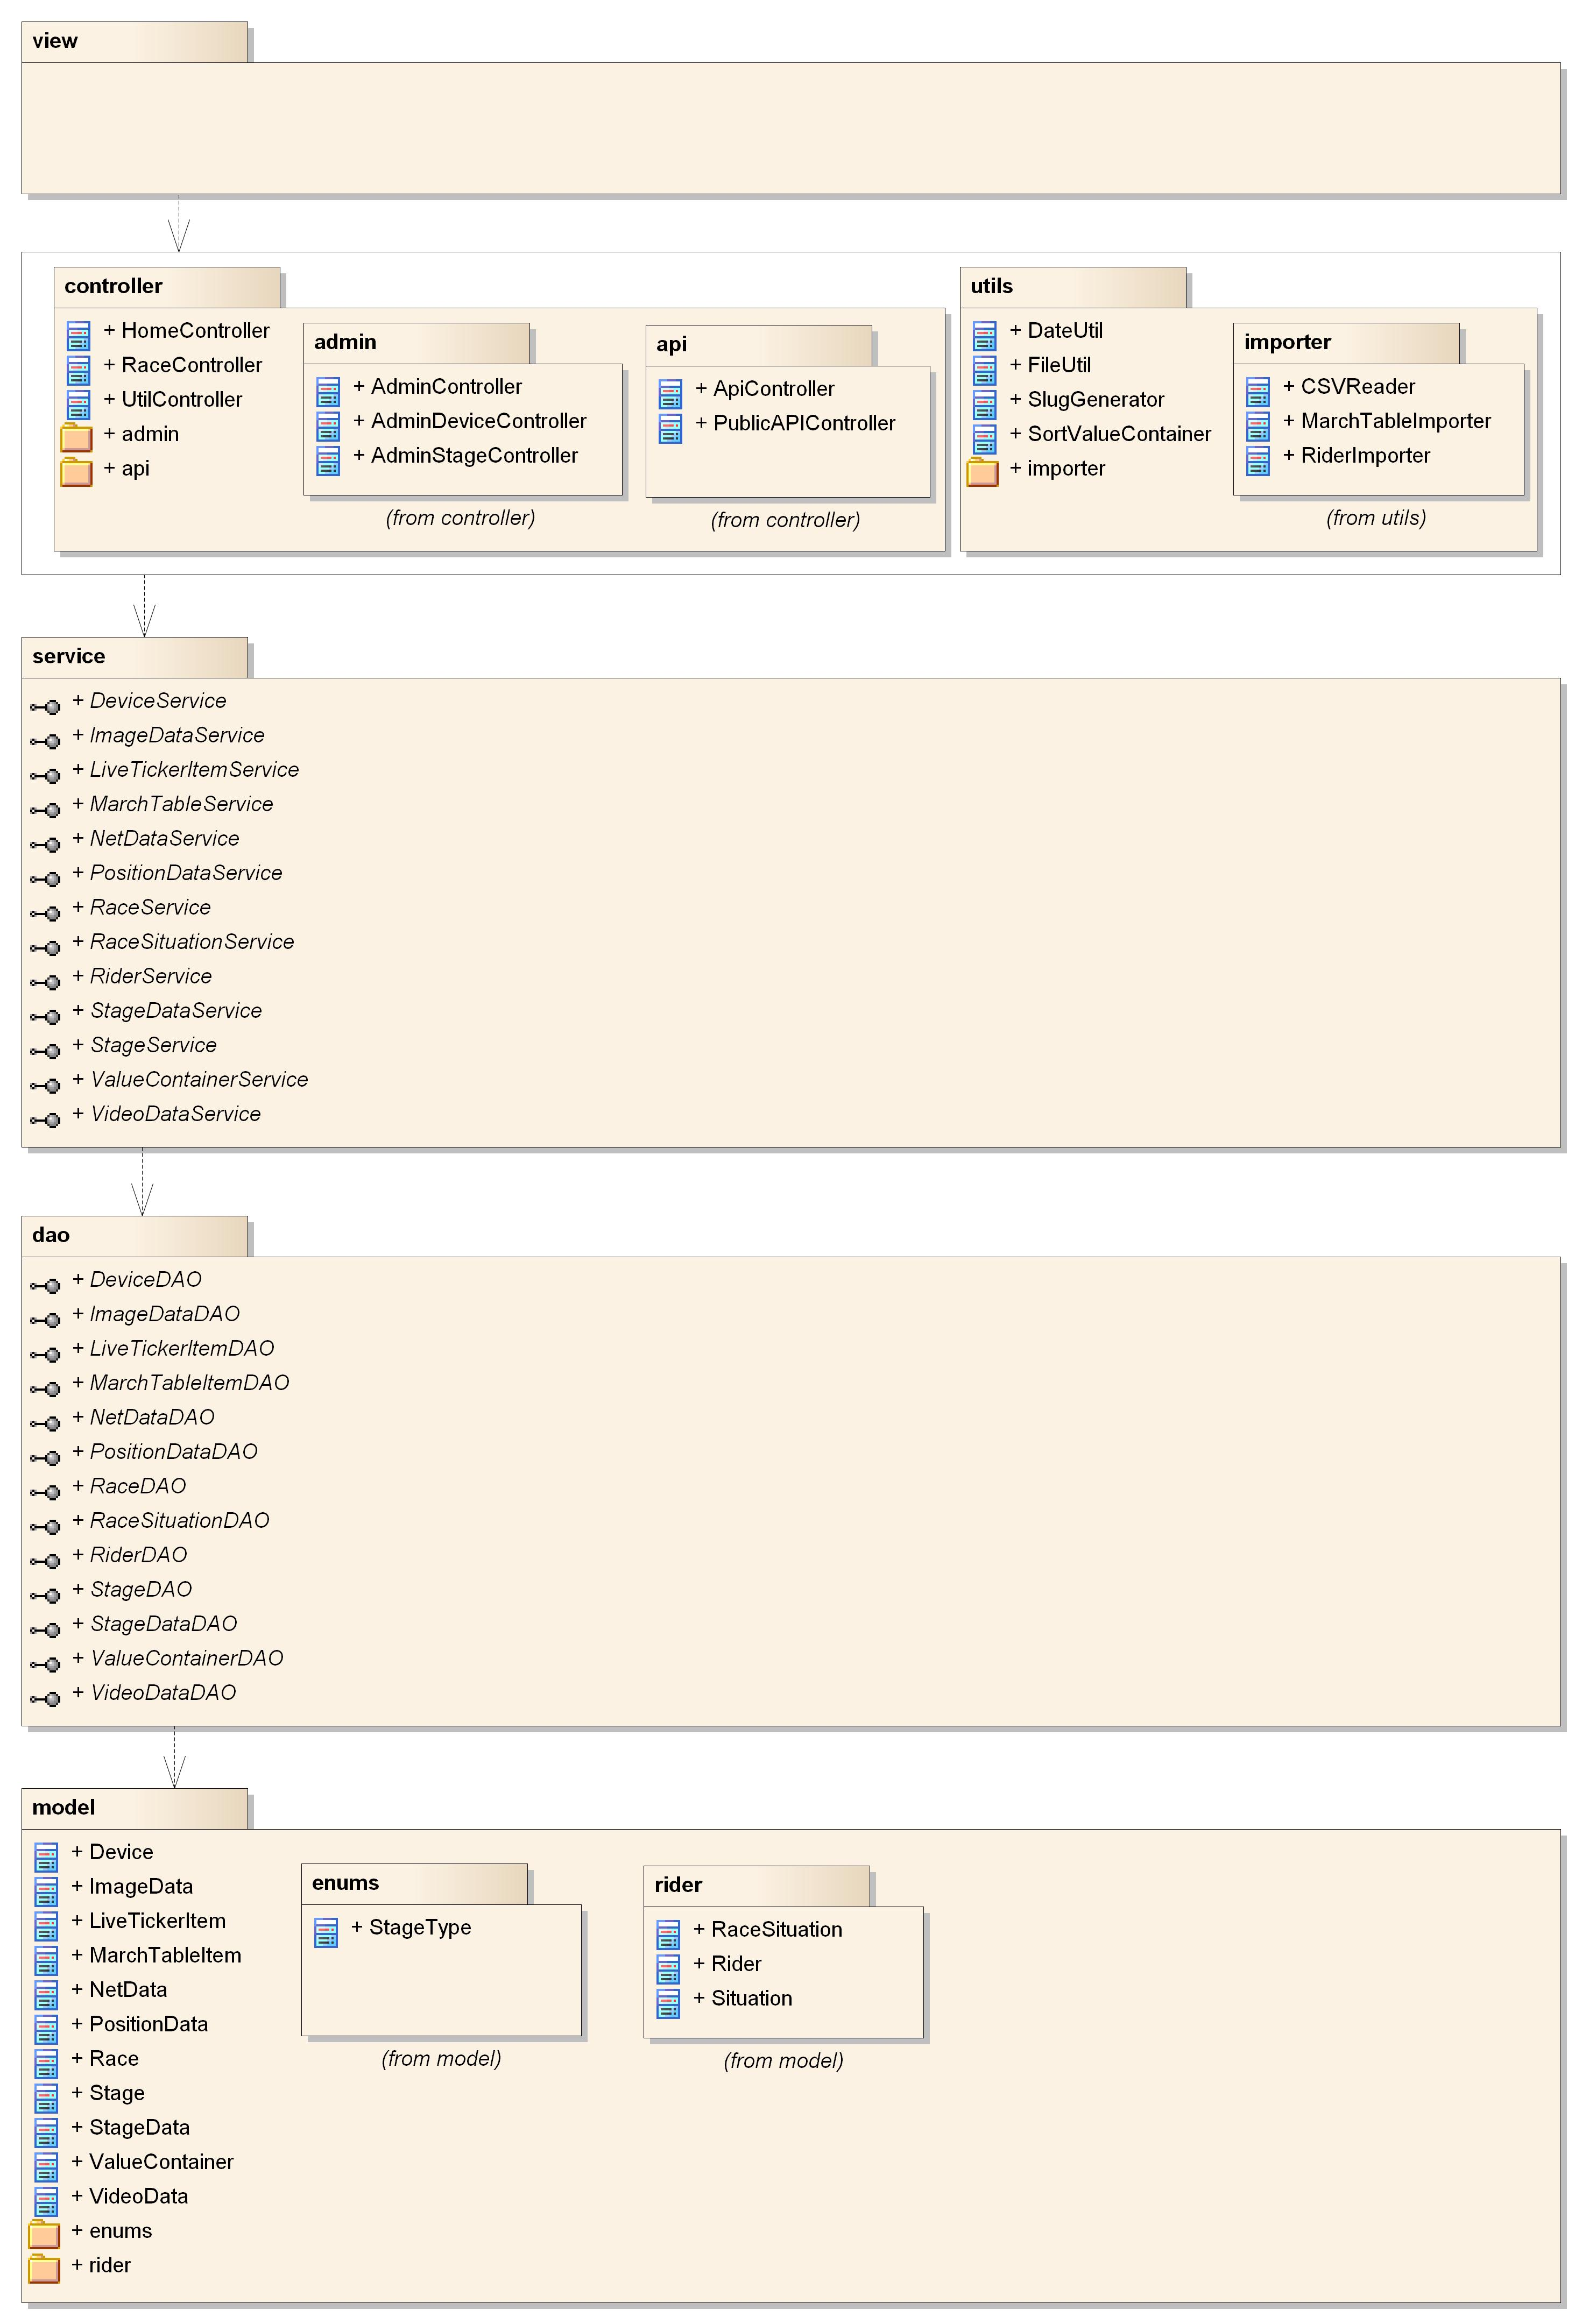
\includegraphics[width=150mm]{images/tourliveweb/TourLiveServer_Package_ohneRand.jpg}
	\caption{Packagediagramm des TourLive Servers}
\end{figure}\label{fig:tourlivewebpackage}

Im Packagediagramm \ref{fig:tourlivewebpackage} sind die Schichten der Applikation zu erkennen. So wurde das Domainmodel im Package \textit{Model} abgebildet, die Datenzugriffsobjekte im \textit{DAO} Package und die dazugehörige Service Schicht im Package \textit{Service}. Die Anfragen werden durch die Zugriffscontroller im Package \textit{Controller} bearbeitet. Um wiederkehrende Tasks zu zentralisieren, wurden diese im Package \textit{Utils} zusammengefasst, so z.B. das Formatieren Zeiten und Daten.

\subsection{Video}
Eine Anforderung war es, eine Lösung zu erarbeiten, welche es ermöglicht mit den Aufnahmegeräten Video Streams aufzuzeichnen und an den Server zu übermitteln. Dazu gibt es verschiedene Ansätze mit entsprechenden Vor- und Nachteilen. Im TourLive System im Einsatz ist eine eigene Entwicklung welche genau auf die Bedürfnisse angepasst ist. Die Geräte nehmen Videosequenzen auf und übertragen diese an den Server. Der Server konvertiert diese Sequenzen vom mp4 in das ogg Format. Dazu wird die externe Library Xuggler\footnote{Xuggler, \url{http://www.xuggle.com/xuggler}, aufgerufen am 04.06.2013} verwendet. Mit diesem Schritt sind die Browser Google Chrome, Mozilla Firefox und Microsoft Internet Explorer fähig die Videosequenzen abzuspielen. Zusätzlich wird ein VideoData Objekt (vgl. Abbildung \ref{fig:tourliveserverdomainmodel}) in der Datenbank angelegt, welches den Aufnahmezeitpunkt und die Geräte ID, eine allfällige Rotation, sowie den Pfad zur Videodatei enthält. Wenn nun ein Gerät einer Etappe zugewiesen ist und Videosequenzen vorhanden sind, wird die aktuellste Sequenz ausgeliefert. Der Videoplayer meldet wenn die Videosequenz beendet ist und lädt, falls möglich, die nächste Sequenz via AJAX automatisch nach, dies wird im Quellcode \ref{code:ajaxquellcode} dargestellt. Falls kein neues Video verfügbar ist, wird nach 8 Sekunden erneut versucht ein Video zu laden. Dadurch wird auch bei einem temporären Ausfall der Aufnahmegeräte die Videowiedergabe fortgesetzt, sobald diese wieder verfügbar ist.

\begin{lstlisting}[language=JavaScript, caption=Automatisches Nachladen von Videosequenzen, label=code:ajaxquellcode]
var videoPlayer1 = document.getElementById('video1');
videoPlayer1.addEventListener('ended', function(){
	loadNext(videoPlayer1);
});

function loadNext(videoPlayer){
	$.ajax({
		type : "POST",
		dataType: "json",
		url : "/meineetappe/nextvideo",
		data : {
			deviceId : 'meinedeviceid',
			afterId: videoPlayer.id,
		},
		success : function(data) {
			if (data){
				$('#mp4').attr('src', 'http://media.tourlive.ch/'+ data.videoLocation + '.mp4');
				$('#ogg').attr('src', 'http://media.tourlive.ch/'+ data.videoLocation + '.ogg');
				videoPlayer.id= "video" + data.videoDataId;
				videoPlayer.load();
			} else {
			// try again in 8s
				window.setTimeout(function(){loadNext(videoPlayer)},8000);
			}
		}
	});
\end{lstlisting}

\subsection{Bilder}
Die Aufnahme der Bilder funktioniert nach einem ähnlichen Muster. Die aufgezeichneten Bilder werden auf dem Server abgelegt und ein ImageData Objekt in der Datenbank erzeugt. Im ImageData Objekt wird, wie schon beim Video, der Aufnahmezeitpunkt, die Geräte ID sowie der Bildpfad gespeichert. Wie in Abbildung \ref{fig:bildaufzeichnung} zu sehen ist, wird beim Aufruf einer Seite das aktuellste verfügbare Bild pro Gerät angezeigt und mit dem Aufnahmezeitpunkt beschrieben.
\begin{figure}[H]
	\centering
	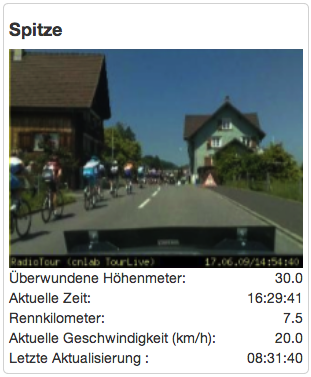
\includegraphics[width=70mm]{images/tourliveweb/bildaufzeichnung.png}
	\caption{Aufgezeichnetes Bild mit Informationen ergänzt}
	\label{fig:bildaufzeichnung}
\end{figure}

\subsection{Positions Daten}
Die Positions Daten werden in Form eines ValueContainers gespeichert und übertragen. Ein beispielhafter ValueContainer ist im folgenden in der JSON Notation dargestellt.

\begin{figure}[H]
	\centering
	\lstinputlisting[language=json]{jsonfiles/valuecontainer.json}
	\caption{Beipsiel ValueContainer in der JSON Notation}
	\label{fig:valuecontainerjson}	
\end{figure}

Der Container setzt sich aus den drei Objekten \textit{netData}, \textit{positionData} und \textit{stageData} zusammen, hinzu kommt zu jedem Container das Device Objekt sowie der aktuelle Zeitpunkt als Timestamp. Daher auch der Name ValueContainer, weil darin verschiedene Daten gesammelt und übermittelt werden.
\\

Die ValueContainer bilden das Herz der Informationsquelle. Alleine durch sortieren nach dem Feld \textit{distance} im Objekt \textit{stageData} wird festgestellt, welches Gerät an der Spitze mitfährt und wie viel Prozent der Gesamtstrecke zurückgelegt wurde. Da die ValueContainer nicht einer Etappe sondern einem Gerät zugeordnet sind, können auch nachträglich noch Geräte einer Etappe hinzugefügt oder entfernt werden. Um die Positionsdaten für eine Etappe zu erhalten werden alle ValueContainer vom Startzeitpunkt bis zum Endzeitpunkt einer Etappe gefiltert und alle mit der Geräte ID eines Gerätes welches der Etappe zugeordnet ist ausgewählt. Um ein vergangenes Rennen wieder abzuspielen wird einfach die zeitliche Grenze welche durch die Etappenendzeit gegeben war ersetzt durch einen beliebigen Zeitpunkt ( > Startzeit). Dadurch werden immer nur diejenigen Container ausgewählt, welche bis zum angezeigten Zeitpunkt aufgezeichnet wurden.
\\

Um die Daten zu visualisieren werden verschiedene Elemente verwendet. Der geografische Verlauf der Strecke wird auf einer Karte eingezeichnet. Jedes Aufnahmegeräte (\textit{device}) hat zusätzlich ein Feld \textit{color}, welches die Farbe auf der Karte bestimmt.
\begin{figure}[H]
	\centering
	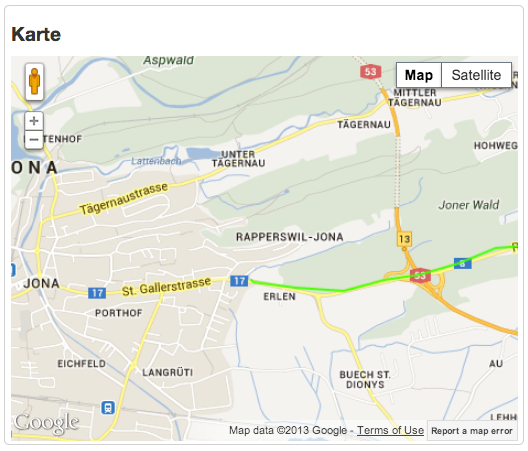
\includegraphics[width=110mm]{images/tourliveweb/karte_neu.png}
	\caption{Kartenausschnitt mit zurückgelegter Strecke eines Gerätes}
\end{figure}

Ein Aufnahmegerät fährt in der Regel an der Spitz mit, ein zweites hinter dem Feld. Die Spitze setzt sich im laufe des Rennens ab und der Abstand wird grösser. Die Entwicklung dieses Abstands ist für Radsportbegeisterte sehr spannend zu beobachten. Diese Berechnung wird ebenfalls durch die ValueContainers ermöglicht. Sobald mehr als ein Gerät einer Etappe zugeordnet ist, beginnt die Berechnung des Abstandes nach dem folgenden Algorithmus.
\begin{quotation}
\textit{Für jeden ValueContainer in einer Etappe mache folgendes:
Suche pro Gerät den ValueContainer welcher die nächsttiefere Etappendistanz im Vergleich zum obigen Container aufweist, falls dieser Distanzunterschied kleiner als eine definierte Grösse ist (Standardwert 500m) so wähle den Container mit der kleinsten Zeit. Vergleiche diese Zeit mit dem ursprünglichen Container, ist die Zeit des ursprünglichen Containers grösser, so ist die Differenz der Zeiten den Rückstand für diesen Container, andernfalls ist der ursprüngliche Container zu dem Zeitpunkt an der Spitze}
\end{quotation}

Diese Berechnung ist sehr Aufwändig und wird mit steigender Anzahl ValueContainers immer langsamer. Im lokalen Testumfeld mit weniger als 1000 ValueContainer wird diese Berechnung kaum bemerkt. Beim ersten Testlauf stellte sich jedoch heraus, dass diese Werte zwischengespeichert werden müssen, da die Liveberechnung einfach zu lange dauern würde. Bei jedem Seitenaufruf werden nur die neu hinzugekommenen ValueContainer berechnet, dadurch wird das System quasi schneller, je mehr Benutzer auf der Seite sind, da die Anzahl neu zu berechnender Werte immer kleiner wird. Im Administrationsbereich kann die manuelle Berechnung aller ValueContainer neu gestartet werden. Dieser Vorgang ist notwendig, wenn nachträglich ein weiteres Gerät zur Etappe hinzugefügt wird.
\\

Sämtliche Rückstände werden in einer Grafik (vgl. Abbildung  \ref{fig:abstandsentwicklung2}) dargestellt. In der X-Achse sind die zurückgelegten Rennkilometer und in der Y-Achse die Rückstände in Sekunden. Für das Aufnahmegerät an der Spitze ist diese Kurve komplett flach, daher wird diese weggelassen.

\begin{figure}[H]
	\centering
	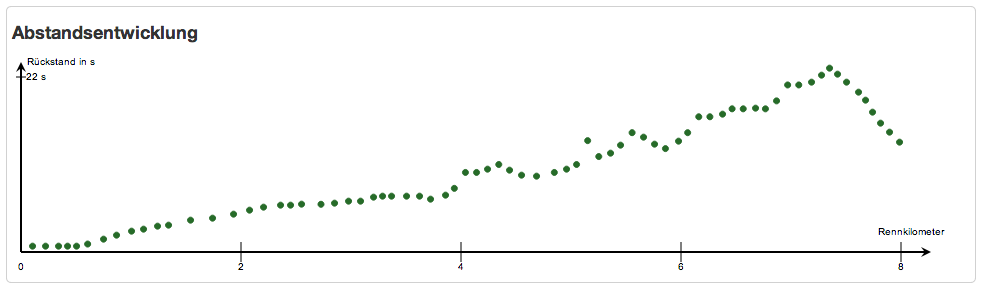
\includegraphics[width=130mm]{images/tourliveweb/abstandsentwicklung2.png}
	\caption{Abstandsentwicklung am Ende eines fiktiven Rennens}
	\label{fig:abstandsentwicklung2}
\end{figure}

\subsection{Interne API}
Mit der internen \gls{api} wird die Schnittstelle zwischen den Aufnahmesystemen und dem TourLive Server bezeichnet. Diese Schnittstelle wird genauer im Kapitel \ref{sec:tourliveserverapi} erklärt.

\subsection{Public API}
Für die aufgezeichneten Daten wurde ebenfalls eine öffentliche Schnittstelle erstellt. Drittentwicklern wird es ermöglicht die Positionsdaten in ihren Anwendungen zu verwenden und die Bilder als auch die Videosequenzen abzurufen. Die Schnittstelle ist zum jetzigen Zeitpunkt uneingeschränkt nutzbar. Für den produktiven Betrieb von TourLive wäre eine Authentifizierung für die Benutzung der Schnittstelle wünschenswert, eine solche ist aber nicht Teil dieser Arbeit. Die öffentliche Schnittstelle ist im Kapitel \ref{sec:tourlivepublicapi} detailliert beschrieben.

\subsection{XML basierte Konfiguration}
Die Konfiguration in Spring geschieht einerseits über Java Annotationen wie Sie beim TourLive Server z.B. bei den Controllern zum Einsatz kommen, andererseits werden Servlet und Datenbankeinstellungen sowie sämtliche Abhängigkeiten zu anderen Libraries in XML Dateien konfiguriert. Die wichtigsten Dateien werden im folgenden aufgezeigt.

\subsubsection{web.xml}
Im web.xml wird zugewiesen welches Servlet welche Ressource ansteuert. Weiter werde die Filter definiert, welche angewendet werden sollen. Filter erlaube es Anfragen vor oder nach zu bearbeiten. Im TourLive Server werden die zwei Filter verwendet, zum einen der Sitemesh Filter welcher wiederverwendbare Elemente (z.B. Menu oder Footer) in den JSP Seiten auslagert. Der zweite Filter schützt den Administrationsbereich vor nicht authentifiziertem Zugriff. Bei diesem Security Filter kann eine Ressource komplett geschützt werden. Die weitere Konfiguration findet dann in der security.xml Datei statt.

\subsubsection{tourlive-servlet.xml}
Damit die von den Controllern erstellten Models auch auf den JSP Seiten abgebildet werden können wird ein ViewResolver verwendet. In der XML Datei wird zusätzlich angegeben wo sich die JSP Seiten befinden. Weiter werden die Internationalisierung und die Auslieferung von statischen Ressourcen, wie Bilder und StyleSheets, definiert.

\subsubsection{hibernate.xml}
Das Datenbankmapping geschieht mit Hibernate. In der hibernate.xml Datei werden die Datenbankeinstellungen vorgenommen. Zusätzlich wird hier die SessionBean deklariert, damit werden die Abfragen auf der Datenbank letztendlich ausgeführt.

\subsubsection{root-context.xml}
Im Root Context wird definiert, dass die weitere Konfiguration durch Java Annotationen interpretiert werden soll. Weiter werden die Konfigurationen der Datenbank sowie umgebungsspezifische Einstellungen importiert. Das Pendant zum Root Context für die Testumgebung ist der Test Context.

\subsubsection{security.xml}
Die Sicherheitsparameter welche von Spring geladen werden, sind in der security.xml Datei definiert. So kann eine Login und eine Logout Seite angegeben werden. An dieser Stelle wird auch definiert, dass sämtliche Zugriffe auf die Administrationsseiten nur nach Authentifizierung stattfinden können.
\\

Die TourLive Server Anwendung verfügt nur über zwei Benutzergruppen, nicht authentifizierte Besucher und Administratoren. Daher wurde auf eine Aufwändige Benutzerverwaltung verzichtet und nur ein Administrationsbenutzer fest in der XML Datei definiert.

\section{Realisierung}
Der für die Öffentlichkeit sichtbare Teil dieser Arbeit besteht aus den aufbereiteten Daten. Auf der Startseite wird jeweils die aktuellste Etappe angezeigt alle anderen Rennen können über die Navigation im Kopfbereich erreicht werden. In der Abbildung \ref{fig:tourlivewebansicht} ist ein fiktives Beispiel der ersten Etappe der Tour de Suisse 2013 dargestellt.

\begin{figure}[H]
	\centering
	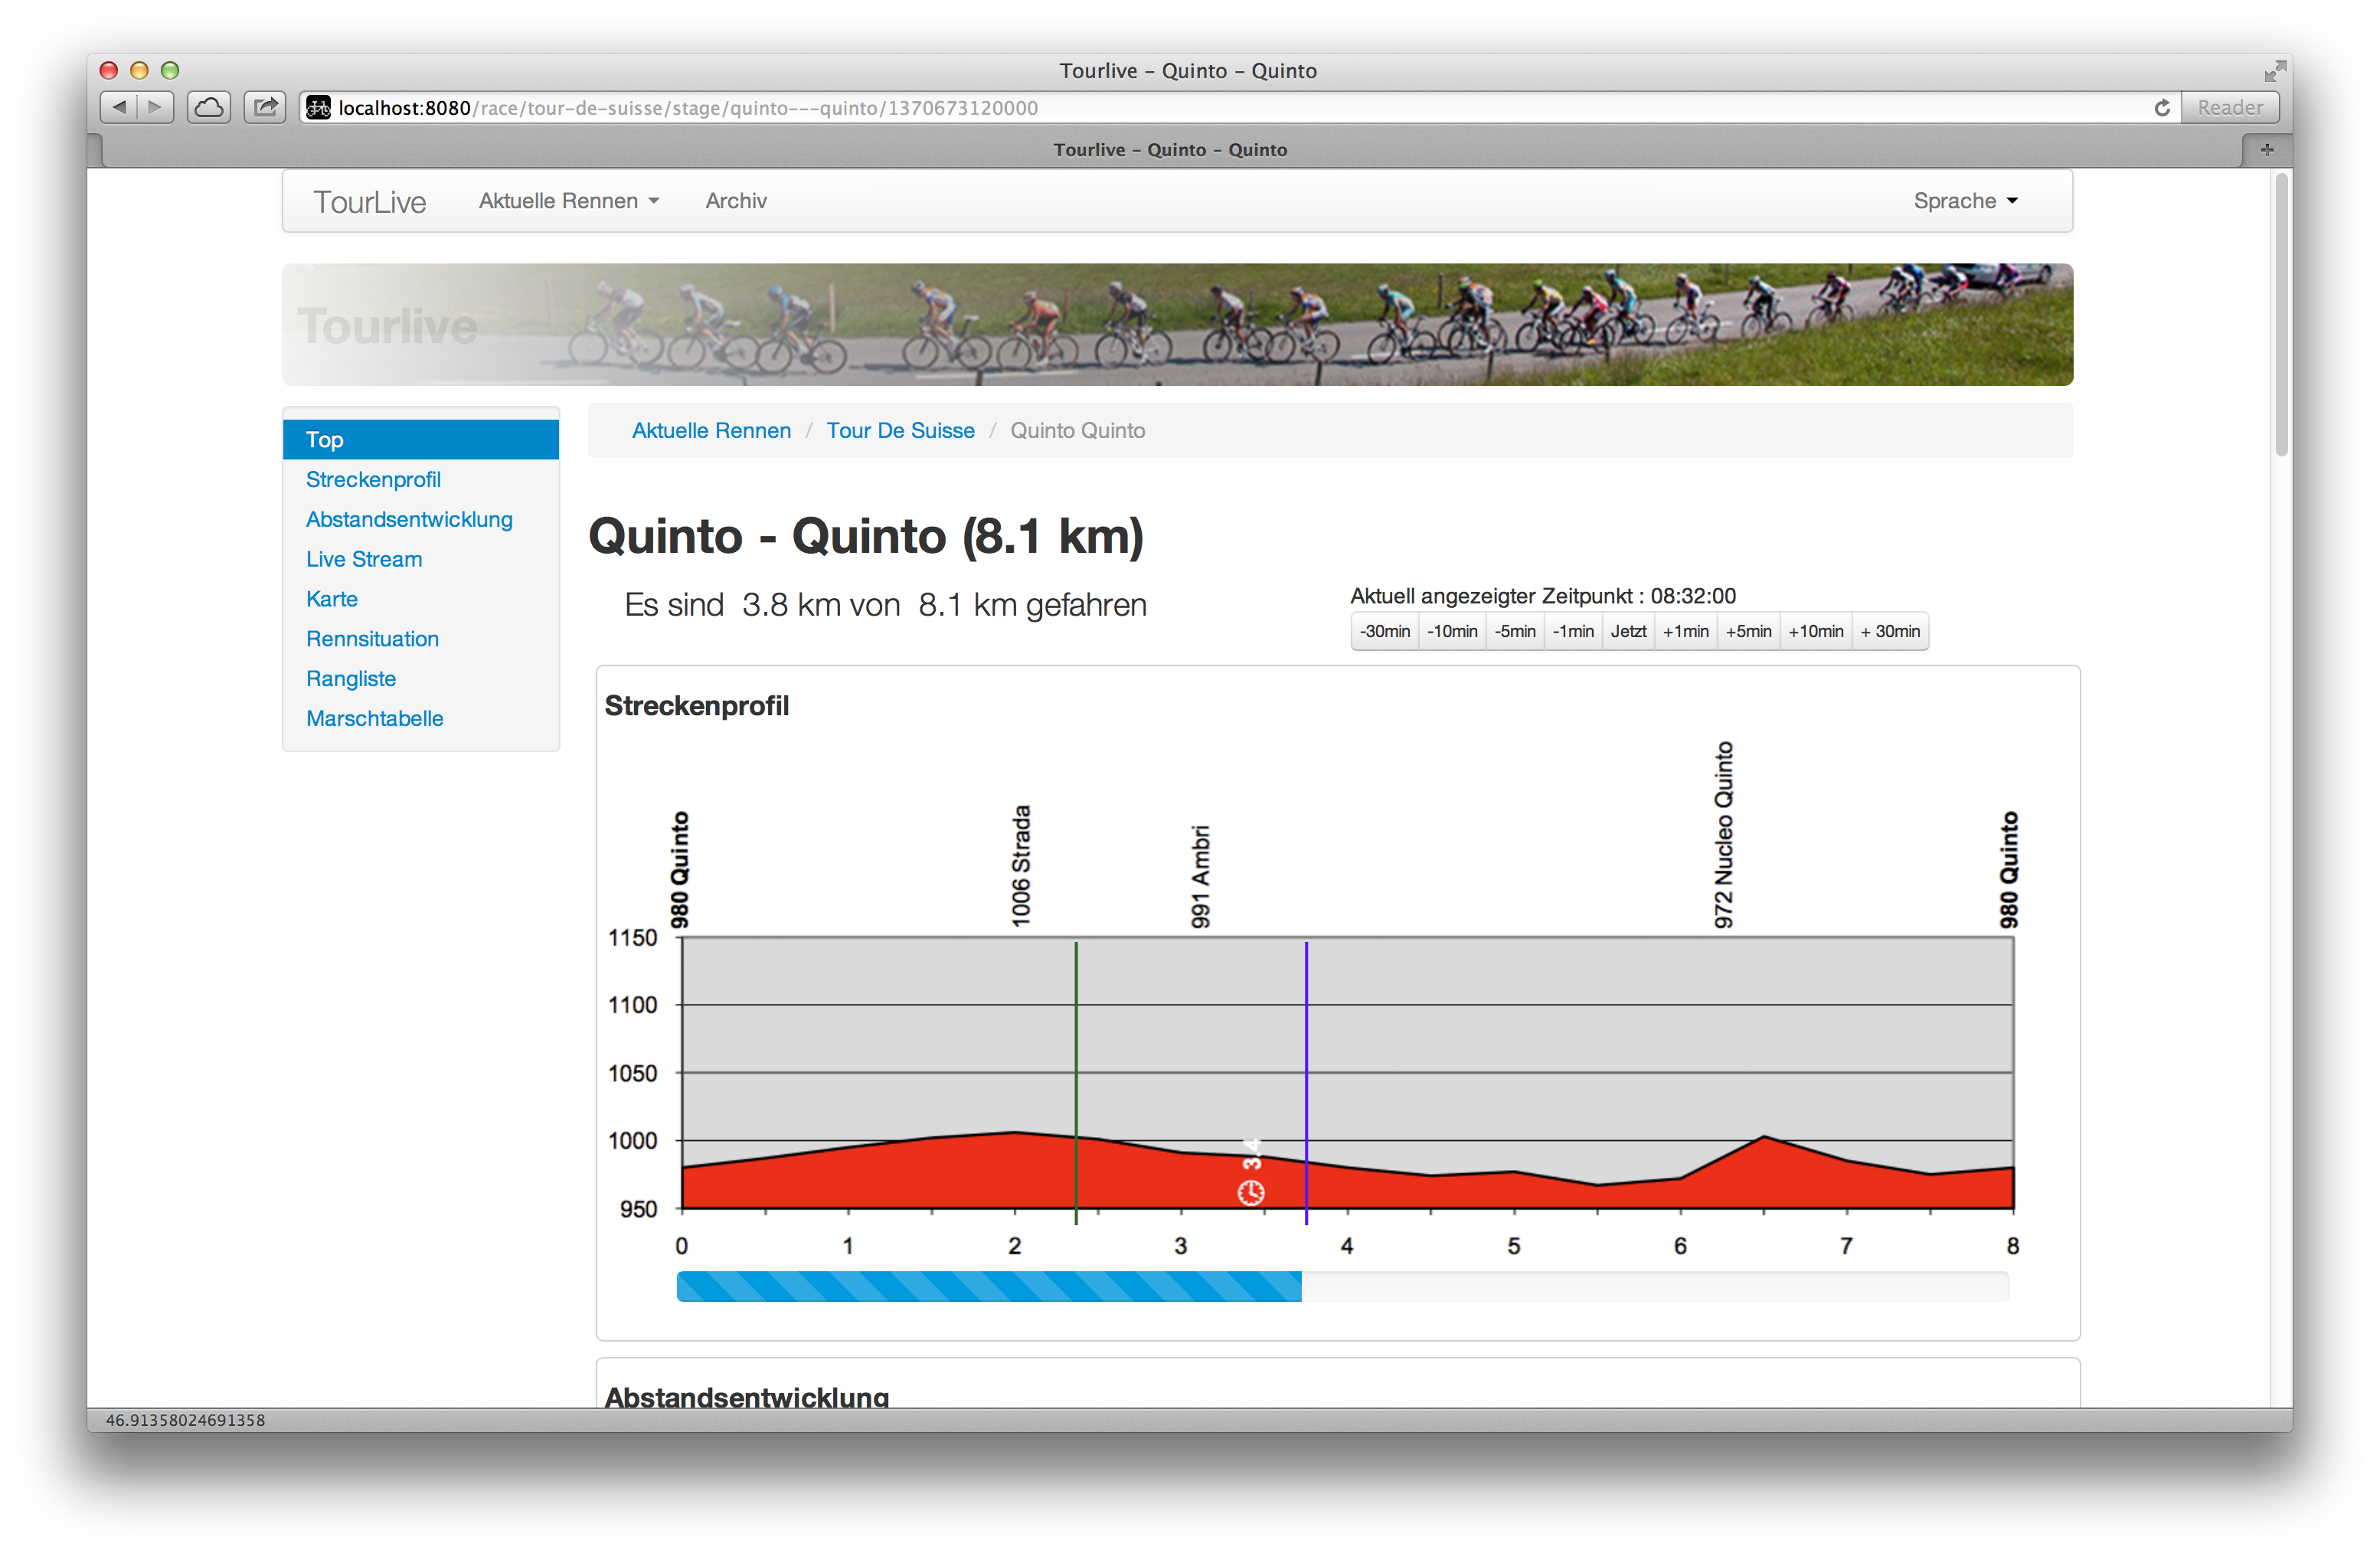
\includegraphics[width=130mm]{images/tourliveweb/tourlivewebansicht.png}
	\caption{TourLive Server Webseite anhand eines Beispiels}
	\label{fig:tourlivewebansicht}
\end{figure}

\subsection{Streckenprofil}
Die aktuelle Positionen der Aufnahmegeräte wird mittels eines HTML5 Canvas direkt auf das Etappenprofil gezeichnet. Dazu wird die JavaScript Library \textit{Raphaël JS}\footnote{Raphaël JavaScript Library, \url{http://raphaeljs.com/}, aufgerufen am 01.06.2013} verwendet. Zu jedem Gerät wird der aktuellste ValueContainer gesucht und daraus die Etappendistanz gelesen. Diese Distanz wird dann relativ zur Seitenbreite des Browserfensters als feine Linie mit der Farbe des Gerätes eingezeichnet wie in der Abbildung \ref{fig:tourlivewebansicht} zu sehen ist. Gleich unterhalb dieser Grafik befindet sich eine Statusanzeige [blau]. Sie zeigt die zurückgelegten Kilometer in dieser Etappe an und dient gleichzeitig auch als Navigation. Durch klicken an einer beliebigen Stelle im blauen Balken kann man zu dieser Stelle (Rennkilometer) im Rennen zurückspringen. Das Pendant zu dieser Navigation sind die Schaltflächen im oberen Bereich, welche das Rennen über die Zeit navigieren lassen.
\\

Gleich wie die Positionen der Aufnahmegeräte werden auch die Daten der Abstandsentwicklung mit der Raphaël JavaScript Library dargestellt.


\chapter{Device Management Server}
\label{sec:devmgmtsrv}

In den folgenden Abschnitten wird die Webapplikation Device Management Server erläutert. Dabei liegt der Fokus auf der Spezifikation und deren technischen Umsetzung. Dieses Kapitel richtet sich ins Besondere an Entwickler, welche an diesem Projekt weiterarbeiten möchten und an Personen, welche an den technischen Details interessiert sind.

\section{Software Analyse}

\subsection{Anforderungen}
Um die Anforderungen zu evaluieren wurde das bestehende Geräteverwaltungsportal analysiert. Da beim bestehenden System der Funktionsumfang stark eingeschränkt war, wurde vom Industriepartner zusätzliche Funktionalität gewünscht.
Um eine kurze Übersicht über die vorhandenen Funktionen und erfassten Anforderungen zu geben folgt  eine Tabelle.

\begin{longtable}{  p{3.5cm} | p{4.3cm} | p{4.3cm} }

    \textbf{Anforderung} & \textbf{Altes System} & \textbf{Neues System} \\ [1ex] \hline \hline & &  \\ [-1.5ex]
    Einstellungen anpassen & Nur Renndistanzkorrektur & Detaillierte Verwaltung der Geräteeinstellungen\\ [1ex] \hline & &  \\ [-1.5ex]
    Status der Geräte & Rudimentäre Anzeige des Gerätestatus & Detaillierte Anzeige des Gerätestatus\\ [1ex] \hline & &  \\ [-1.5ex]
     Alarming bei schlechtem Gerätezustand & Dauer seit letztem Positionsupdate / Bildempfang zu gross & Visuelle Hervorhebung bei Problemen mit dem Gerätestatus \\ [1ex] \hline & &  \\ [-1.5ex]
    Neustarten des Gerätes & Neustarten des Gerätes via Portal & nur Neustarten der App möglich\\ [1ex] \hline & &  \\ [-1.5ex]
    Gerätelog anzeigen & - & Gerätelog anzeigen\\ [1ex] \hline & &  \\ [-1.5ex]
    Versand von Nachrichten & - & Versand von Nachrichte möglich\\ [1ex] 
\caption{Anforderungen Device Management Server}
\end{longtable}

Eine detaillierte Beschreibung aller Anforderungen befindet sich im Anhang im Kapitel  \ref{sec:anforderungenandroiddevmgmt}. Nachfolgend werden die wichtigsten Anforderungen beschrieben.

\subsubsection{Funktionale Anforderungen}
\paragraph{Betriebsmodi}
Die Geräte sollen sowohl über ein Management Server, analog zur bisherigen Verwaltungsseite , fernverwaltet als auch über ein „Einstellungen“-Menü direkt am Gerät konfiguriert werden können. 

Daraus resultieren zwei Betriebsmodi: «managed» (TourLive App wird über den Device Management Server verwaltet) und «unmanaged» (TourLive App wird in den lokalen App Einstellungen verwaltet). Die Standardkonfiguration sieht den Modus «managed» vor. Die beiden Modi lassen sich jedoch am Gerät wie auch auf dem Device Management Server jederzeit ändern. 


\paragraph{Alarming Funktionen}
Treten Probleme auf, so soll auf dem Telefon sowie in der Management Konsole darüber informiert werden. Als zu meldende Probleme gelten folgende:
\begin{itemize}
\item Keine GPS-Daten während 2 Minuten
\item Keine Bild-Daten während 2 Minuten
\item Keine Verbindung zum TourLive Server während 2 Minuten
\item Smartphone wird nicht mehr geladen (Stromzufuhr unterbrochen)
\item Smartphone Akkustand liegt unter 30%
\end{itemize}
	
\subsection{Technologien}
Für die Entwicklung des Device Management Servers wurden dieselben Technologien verwendet die bereits für den TourLive Server evaluiert wurden. Mehr Informationen dazu im Kapitel  \ref{sec:tourliveserverevaluationwebframework} Evaluation Webframework.

\subsection{Domain Model}
Folgende Abbildung zeigt das Domain Model des Device Management Servers. Das Domain Model kann grundsätzlich in 4 Kategorien unterteilt werden die immer mit einem Gerät (der Klasse Device) assoziiert sind:


\begin{itemize}
\item Die Klasse TourLiveLog mit sämtlichen Gerätelogs in Form der Klasse LogEntry. 
\item Die Klasse DeviceManagementContainer die sämtliche Geräteeinstellungen verteilt auf die Klassen DeviceSettings, RecordingSettings und AdditionalSettings speichert.
\item Die Klasse StatusData die den aktuellen Gesundheitszustand eines Aufnahmegerätes wiederspiegelt.
\item Die Klasse Message die allfällige Nachrichten vom Device Management Server an ein Aufnahmegerät speichert.
\end{itemize}

\begin{figure}[H]
	\centering
	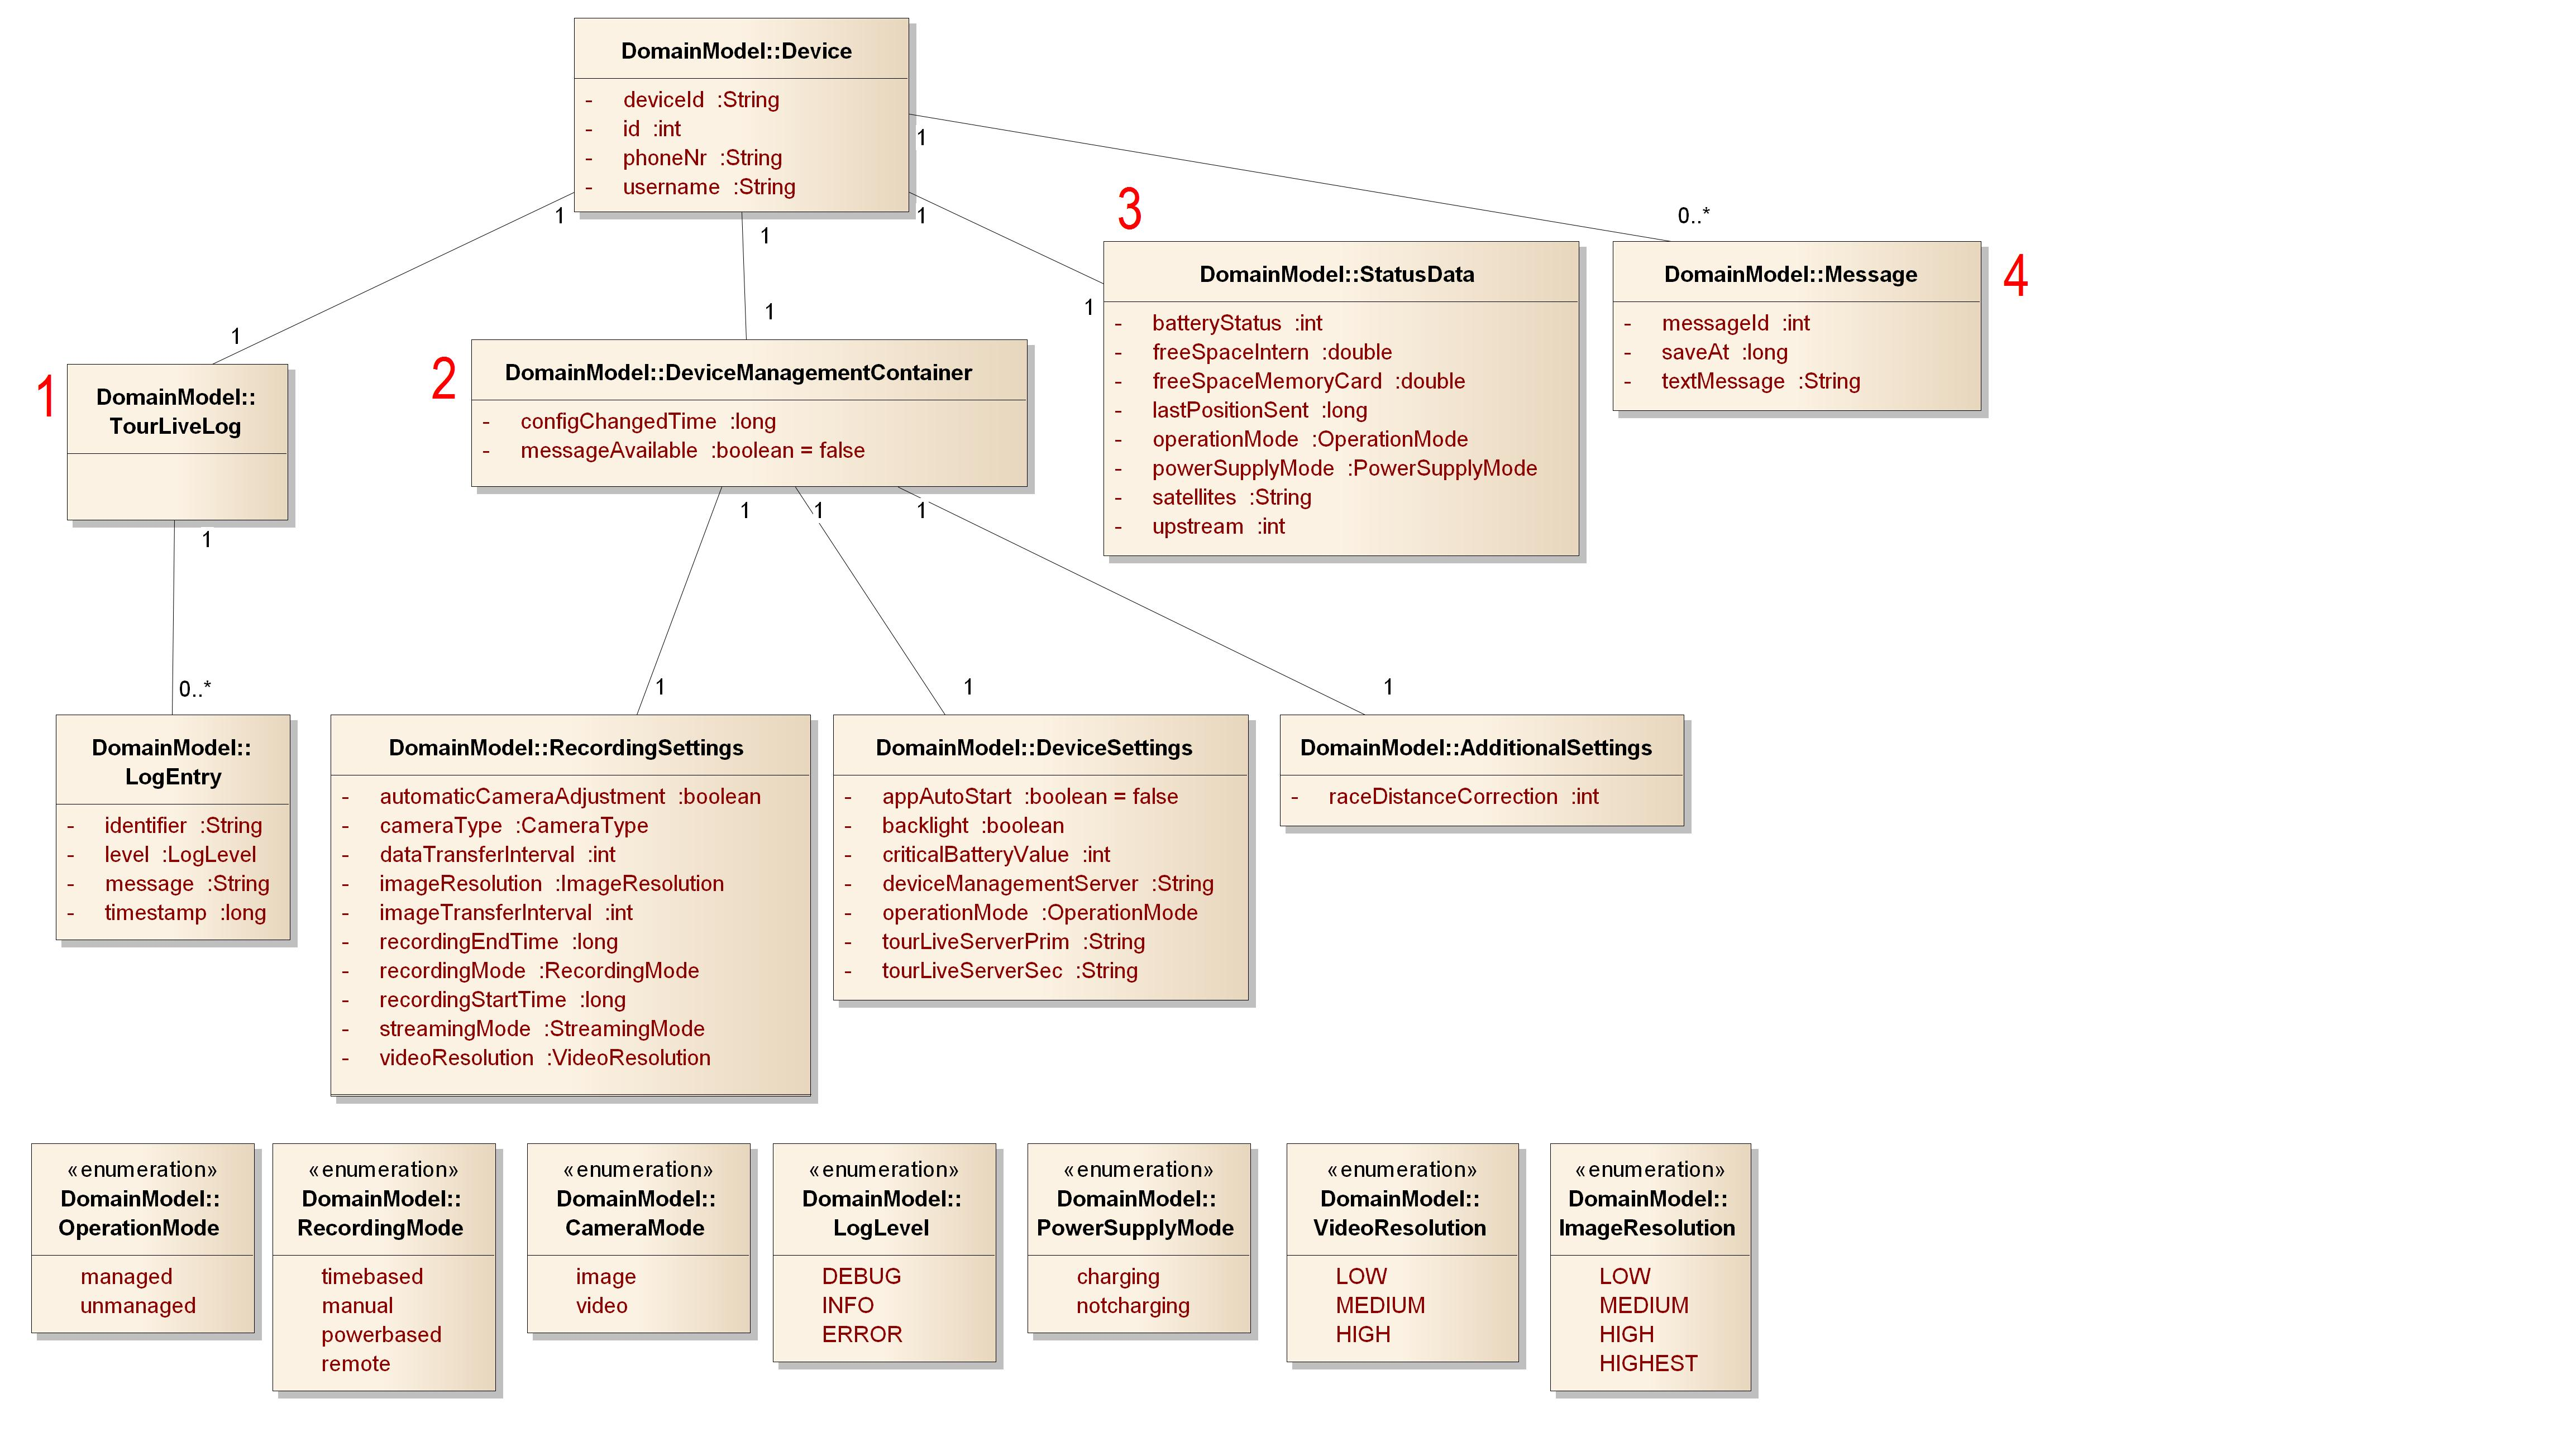
\includegraphics[width=120mm]{images/devmgmtsrv/domainmodel.jpg}
	\caption{Domain Model des Device Management Servers}
\end{figure}


\section{Software Design}
\subsection{Architektur und Übersicht}
Der Device Management Server hat zwei Hauptaufgaben. Zum einen wird die Bearbeitung der Daten ermöglicht und zum anderen wird dem Aufnahmesystemen eine API zur Verfügung gestellt.


\begin{figure}[H]
	\centering
	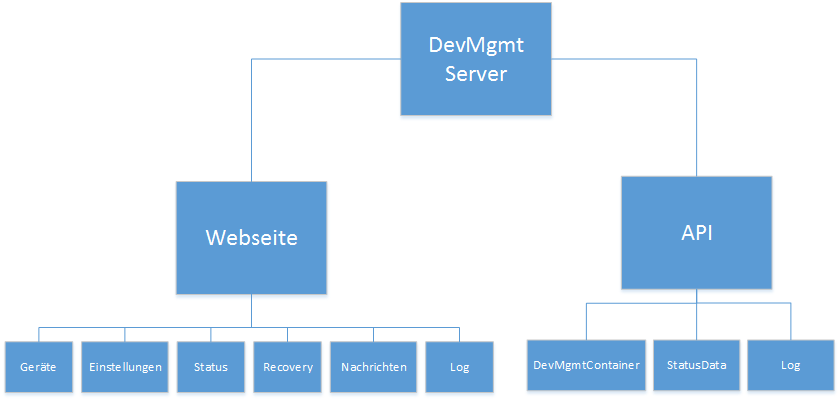
\includegraphics[width=120mm]{images/devmgmtsrv/uebersicht.png}
	\caption{Grobstruktur des Device Management Servers}
\end{figure}

Wie beim TourLive Server besteht dank der gewählten Struktur die Möglichkeit, die Webseite und die API auf verschiedene Server aufzuteilen. Da die Auslastung des Device Management Servers jedoch gering ist, wird darauf nicht weiter eingegangen.

\subsection{Schichtenmodell und Paketdiagramm}
Der Device Management Server ist in vier Schichten unterteilt. Die Schichten wurden an die Struktur des Spring Frameworks angepasst. Folgende Abbildung zeigt diese vier Schichten auf.

\begin{figure}[H]
	\centering
	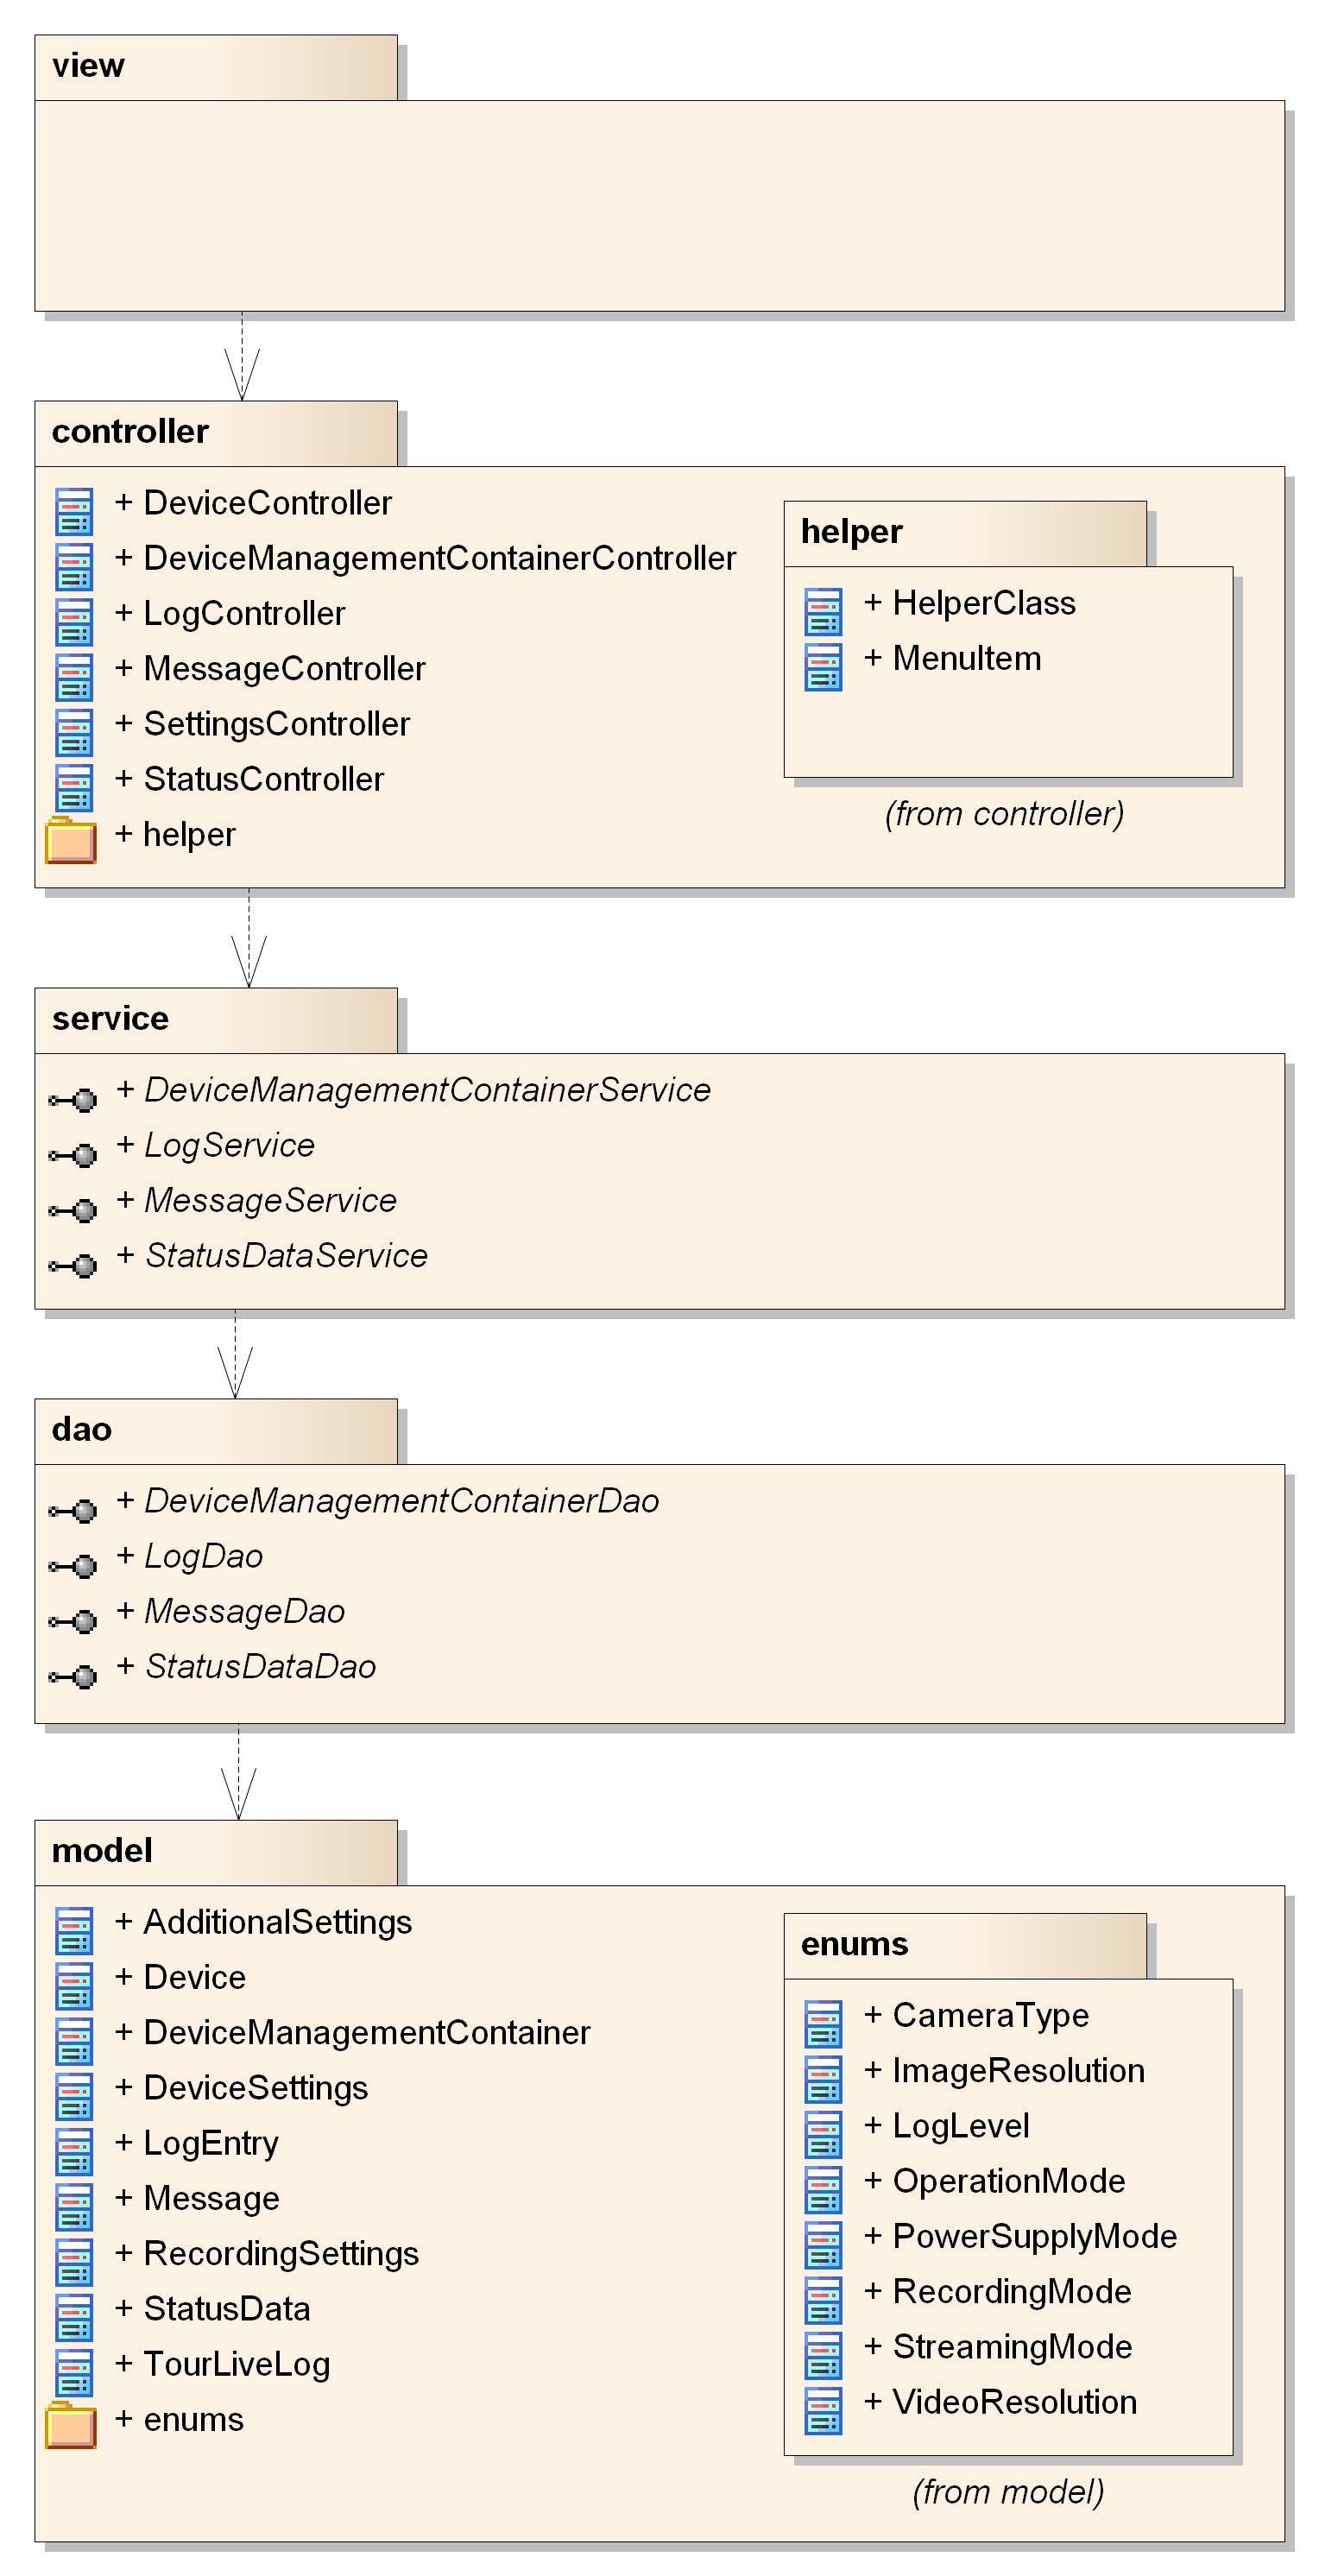
\includegraphics[width=80mm]{images/devmgmtsrv/schichten.jpg}
	\caption{Schichtendiagramm des Device Management Servers}
\end{figure}

\subsubsection{View}
Die View Schicht enthält alle *.jsp Dateien, die für die Darstellung der Webseite benötigt werden. 

\subsubsection{Controller}
Die Controller widerspiegeln die HTTP-Methoden (GET, POST,...) die für die Anzeige der Webseite und die RESTful JSON-Schnittstelle benötigt werden.

\subsubsection{Service}
Die Service Klassen sind für die Businesslogik auf den von den DAO's gelieferten Objekten verantwortlich.

\paragraph{DeviceManagementContainerService}
Der Device Management Container Service speichert und liefert die Container mit den Geräteeinstellungen sowie das Flag \textit{'messageAvailable'} falls auf dem Device Management Portal eine Nachricht für das Gerät vorhanden ist.

\subsubsection{DAO}
Die DAO Schicht enthält die Datenzugriffsobjekte. Diese dient zur Entkopplung der Geschäftslogik vom Datenzugriff. Die Interfaces bilden die Schnittstelle, die Implementierung kann so je nach Persistenztechnologie unterschiedlich sein, ohne dass die Geschäftslogik geändert werden muss.


\subsubsection{Model}
Die Domäne des Device Management Servers wird in der Model Schicht abgebildet. In den Objektinstanzen der Model Klassen sind die eigentlichen Daten gespeichert. Diese Objektinstanzen werden über den OR-Mapper in der SQL-Datenbank gespeichert.



\section{Realisierung}
Folgendes Kapitel beschreibt die Umsetzung des Device Management Servers.

\subsection{API}
Die API wird mittels Spring Annotations definiert. 

\begin{lstlisting}[language=Java, caption=Spring Annotation]
@RequestMapping(value = "/api/getdevmgmtcontainer", method = RequestMethod.POST)
@ResponseBody
public DeviceManagementContainer getDeviceManagementContainer(@RequestBody final StatusData request)

\end{lstlisting}
\textbf{\textit{@RequestMapping}:} gibt an, welche URL auf diese Methode gemappt wird und welche Request Methode erlaubt ist.\\
\textbf{\textit{@ResponseBody}: } definiert, dass die Methode eine Antwort zurück gibt.\\
\textbf{\textit{@RequestBody}: } der Parameter der Methode wird als Body des Requests definiert.\\
Diese annotierten Methoden müssen in einer Klasse enthalten sein, welche als \textit{@Controller} annotiert ist.


\subsection{Webseite}
Die Webseiten wurden mit JSP umgesetzt. Als Erweiterung wurde Javascript sowie das JQuery Plugin verwendet. Um die grafische Oberfläche möglichst einfach zu gestalten, wurde das Twitter Bootstrap \footnote{Twitter Bootstrap, \url{http://twitter.github.io/bootstrap/}, besucht am 25. Mai 2013} CSS benutzt.

Die Webseite wird in drei Teile unterteilt, Header, Footer sowie der Hauptbereich. 

\begin{figure}[H]
	\centering
	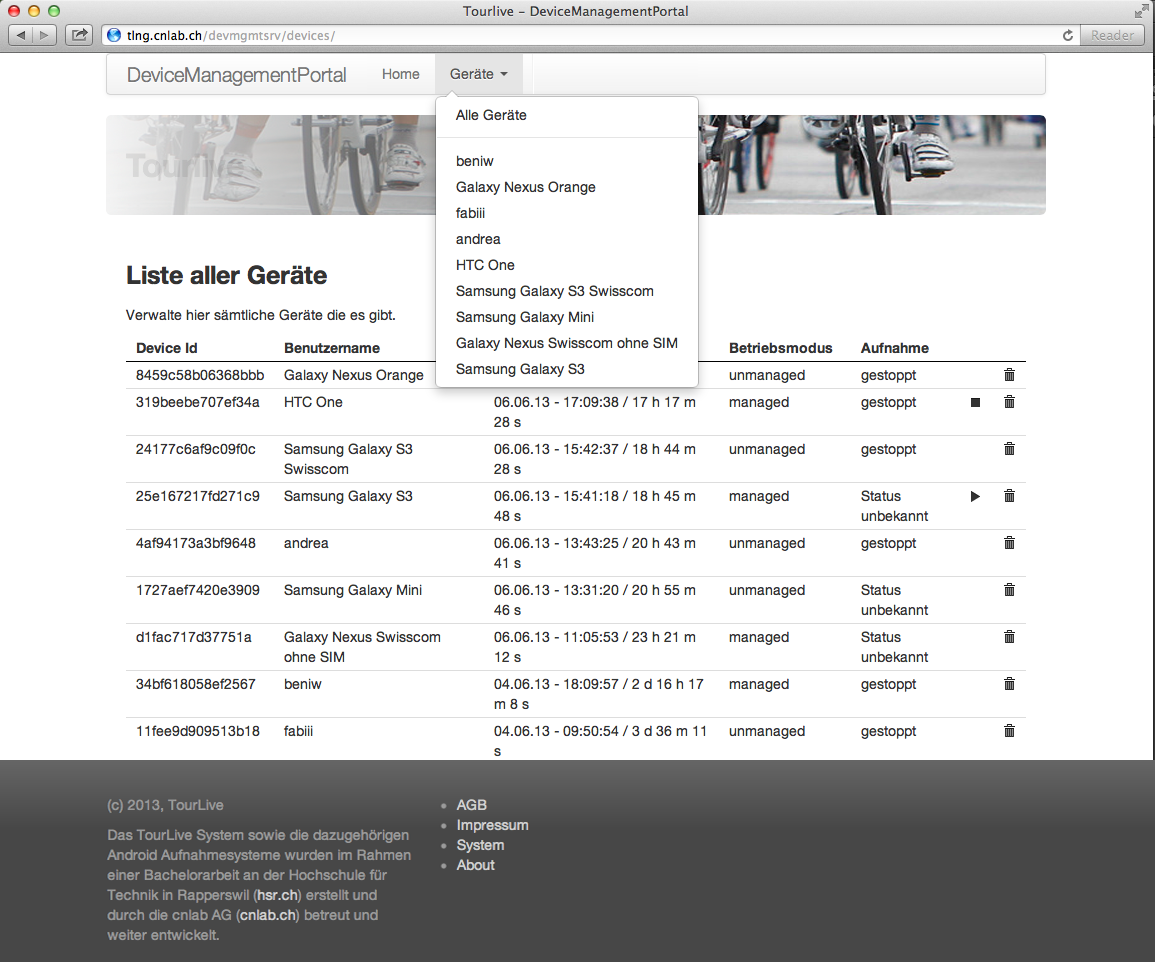
\includegraphics[width=120mm]{images/devmgmtsrv/all.png}
	\caption{Übersicht der DevMgmt Webseite}
\end{figure}

\subsubsection{Header}
Der Header bietet die Möglichkeit, über eine Schnellnavigation auf ein Gerät zuzugreifen. 
\begin{figure}[H]
	\centering
	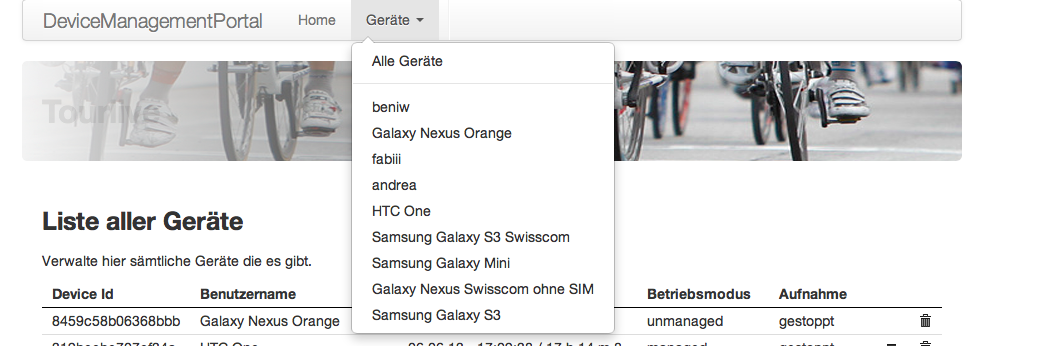
\includegraphics[width=120mm]{images/devmgmtsrv/header.png}
	\caption{DevMgmt Webseite Header}
\end{figure}



\pagebreak
\subsubsection{Footer}
Der Footer enthält detaillierte Informationen zum Projekt TourLive. 
 
\begin{figure}[H]
	\centering
	
\includegraphics[width=120mm]{images/devmgmtsrv/footer.png}
	\caption{DevMgmt Webseite Footer}
\end{figure}


\subsubsection{Hauptbereich}
Der Hauptbereich unterteilt sich wieder in zwei Teile. So hat man Links eine neue Navigation, mit welcher man sich zwischen den verschiedenen Seiten hin und her bewegen kann. 
 
\begin{figure}[H]
	\centering
	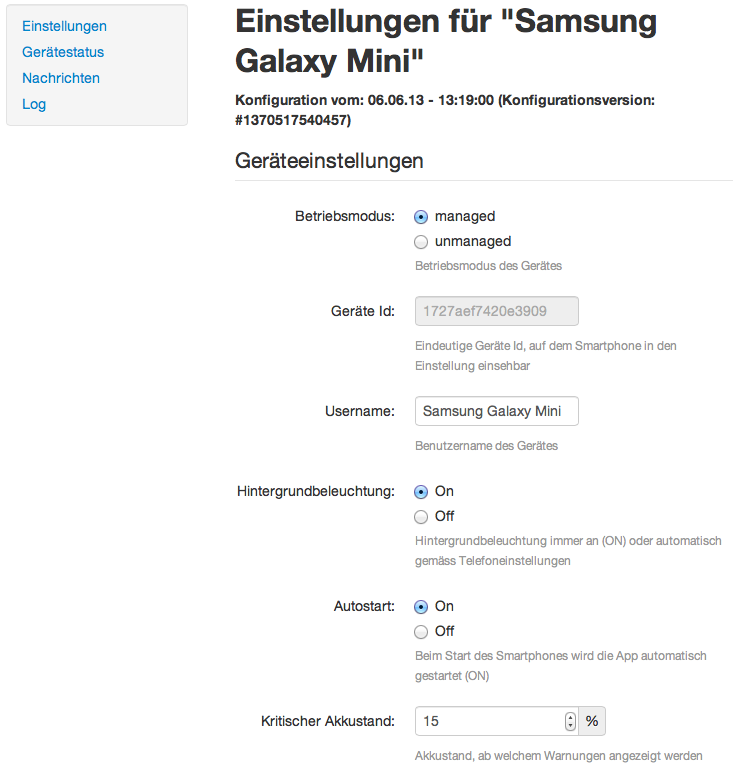
\includegraphics[width=120mm]{images/devmgmtsrv/settings.png}
	\caption{DevMgmt Webseite Hauptbereich}
\end{figure}

\pagebreak
\subsection{Datenbank}
Die Speicherung der Daten in der Datenbank erfolgt mittels Hibernate Annotations.

\begin{lstlisting}[language=Java, caption=Hibernate Annotation]
@Entity
@Table(name = "Device")
public class Device {
	@Id
	@Column(name = "deviceId")
	private String deviceId;
	@Column
	private String username;
	@Column
	private String phoneNr;
}
\end{lstlisting}

\textbf{\textit{@Entity}:} mit dieser Annotation wird angegeben, dass diese Klasse eine gemappte Hibernate Klasse ist.\\
\textbf{\textit{@Table}:} optional, bei der Angabe dieses Attributs, kann der Name der Tabelle definiert werden.\\
\textbf{\textit{@Id}:} definiert das folgende Attribut als Primärschlüssel.\\
\textbf{\textit{@Column}:} das folgende Attribut definiert die Spalte.

\chapter{Android Aufnahmesystem}
\label{sec:androidaufnahmesystem}

Folgendes Kapitel behandelt das auf Google Android basierende Aufnahmesystem. Das Aufnahmesystem besteht aus zwei separaten Android Applikationen mit der Bezeichnung \textit{TourLive.apk} sowie \textit{TourLiveRecoveryService.apk}. Der Fokus folgender Unterkapitel liegt auf den Spezifikationen und der technischen Umsetzung des Aufnahmesystems und ist für Entwickler gedacht, die das Aufnahmesystem gerne erweitern möchten.

\section{Software Analyse}
Dieses Kapitel beschreibt die Anforderungen ans Aufnahmesystem und gibt einen groben Übersicht über die vorhandene Funktionalität.

\subsection{Anforderungen an das Aufnahmesystem}

Um die Anforderungen zu evaluieren wurde das bestehende Aufnahmesystem auf Basis von Nokia Symbian analysiert. Alle vorhandenen Funktionen wurden erfasst und gemeinsam mit dem Industriepartner um weitere ergänzt. 
Eine kurze Übersicht über die bereits bestehenden Funktionen und den neu erfassten Anforderungen liegt in tabellarischer Form vor.

\begin{longtable}{  p{3.5cm} | p{4.3cm} | p{4.3cm} }
    
    \textbf{Requirements} & \textbf{Altes System} & \textbf{Neues System} \\ [1ex] \hline \hline & &  \\ [-1.5ex]
    Positionsdaten übertragen & Geschwindigkeit, H\"{o}he, Richtung/Beschleunigung, Steigung, Longitude, Latitude & Geschwindigkeit, H\"{o}he, Richtung, Steigung, Longitude, Latitude \\ [1ex] \hline & &  \\ [-1.5ex]
    Etappendaten & Zeit, Höhe, Distanz, Durchschnittliche Geschwindigkeit, UTC Zeit, Datum & Zeit, Höhe, Distanz, Durchschnittliche Geschwindigkeit \\ [1ex] \hline & &  \\ [-1.5ex]
     Tour Total & Zeit Total, Zeit Tour, Distanz Total, Distanz Tour, Höhe Total, H\"{o}he Tour & - \\ [1ex] \hline & &  \\ [-1.5ex]
    Netzdaten übertragen & Zellen ID, Location Area, Signal, Akku, Netzwerk, Netzwerk ID & Zellen ID, Area, Signal, Netzwerk ID, Technologie, Datenrate, RTT, Packet Loss\\ [1ex] \hline & &  \\ [-1.5ex]
    Bilder \"{u}bertragen & wird unterstützt & wird unterstützt \\ [1ex] \hline & &  \\ [-1.5ex]
    Videostream \"{u}bertragen & Einzelne Bilder wurden \"{u}bertragen und serverseitig zu einem Stream zusammengef\"{u}gt & Videosequenzen werden \"{u}bertragen und serverseitig zu einem Stream zusammengesetzt\\ [1ex] \hline & &  \\ [-1.5ex]
    Lokales Caching & nur Bilder wurden gecacht & S\"{a}mtliche aufgenommene Daten werden lokal gespeichert\\ [1ex] \hline & &  \\ [-1.5ex]
	Aufnahme- systemstatus \"{u}bertragen & nur der Akkustand wurde an das Device Management Portal \"{u}bertragen & Detaillierte Statusinformation an das Device Management Portal\\ [1ex] \hline & &  \\ [-1.5ex]   
    Betriebsmodi & - & Managed - Einstellungen \"{u}ber das Portal / Unmanaged - Einstellungen am Ger\"{a}t\\ [1ex] \hline & &  \\ [-1.5ex]
	Auto-Start der App & - & App wird beim Ger\"{a}testart automatisch gestartet\\ [1ex] \hline & &  \\ [-1.5ex]
    Externe Ger\"{a}te & ODB (Onboard Diagnose Bus) und Pulsinfo Ger\"{a}te wurden angesteuert & -\\ [1ex] \hline & &  \\ [-1.5ex]
    Smartphone tauglich & Symbian App & Android App\\ [1ex] \hline & &  \\ [-1.5ex]
    Log & Position und Bilder gesendet & Daten, Bilder, Status und Einstellungen gesendet / Exceptions\\ [1ex] \hline & &  \\ [-1.5ex]
    Aufnahmestart Modi & Aufnahme hat automatisch bei App Start gestartet & Manuell, Zeitbasiert, Fernverwaltet oder bei Aktivierung einer externen Stromquelle\\ [1ex] \hline & &  \\ [-1.5ex]
   	Power Management & - & Bei niedrigem Akkustand wird ein Energiesparmodus aktiviert\\ [1ex] \hline & &  \\ [-1.5ex]
    Alarming Funktion & - & Treten Probleme auf, so wird darauf hingewiesen (z.B. keine GPS Daten w\"{a}hrend 2 Minuten)\\ [1ex] \hline & &  \\ [-1.5ex]
    Mehrsprachig- keit & - & Deutsch und Englisch, einfach erweiterbar\\ [1ex] \hline & &  \\ 
    [-1.5ex] Fehlerkorrektur der GPS Daten & - & Ausreisser bei den GPS Daten werden herausgefiltert\\ [1ex] \hline & &  \\ 
    [-1.5ex] Notfallwiederherstel- lung per SMS & wird unterstützt & wird unterstützt\\ [1ex]
    
\caption{Anforderungen Android Aufnahmesystem}
\end{longtable}

Eine detaillierte Beschreibung aller Anforderungen befindet sich im Anhang im Kapitel \ref{sec:anforderungenandroiddevmgmt}.

\section{Software Design}
Dieses Kapitel dokumentiert das Software Design, verwendete Technologien und die Architektur des Aufnahmesystems.

\subsection{Verwendete Technologien}

\subsubsection{Android}
Eine Voraussetzung für das Aufnahmesystem ist, dass dieses in Form einer Android Applikation entwickelt wird. Die native Programmiersprache für Android Applikationen ist Android Java, ein der Java Standard Edition sehr ähnliches Java Derivat. Die Programmierung in Java bringt den Vorteil, dass die gesamte Android-\gls{api} benutzt werden kann. Da sämtliche Komponenten des TourLive Projektes in Java geschrieben sind kann teilweise auf Server- wie auch Clientseite auf dieselben Klassen-Bibliotheken zurückgegriffen werden, was mögliche Inkompatibilitäten vermindert. 

\paragraph{Android Version}
Eine Anwendung wird f"{u}r eine konkrete Android Version (Minimum Required SDK) entwickelt. Im Rahmen dieses Projektes wird als minimale SDK Version Android 4.0 (Versionsname: Ice Cream Sandwich\footnote{Android Ice Cream Sandwich, \url{http://www.android.com/about/ice-cream-sandwich/}, aufgerufen am 29.04.2013}, , API-Level: 14) verwendet. Die Applikation sollte gemäss Android Richtlinien kompatibel mit allen darauffolgenden Android Versionen sein.

\subsubsection{Externe Libraries}
Um den geforderten Funktionsumfang umzusetzen, wird auf folgende zwei externe Bibliotheken zurückgegriffen.

\paragraph{Spring for Android\footnote{Spring for Android, \url{http://www.springsource.org/spring-android}, aufgerufen am 29.04.2013} }
Ein Rest Client für Android von den Entwicklern des Java Spring Frameworks. Der Rest Client bietet die einfache Möglichker von Serialisierung / Deserialisierung von Java Objekten in JSON-Strings. 

Verwendete Version: spring-android-1.0.1

\paragraph{ORMLite\footnote{ORMLite, \url{ormlite.com}, aufgerufen am 02.05.2013}} ORMLite ist eine OpenSource Java Library, welche das Object-Relational Mapping (ORM) übernimmt. ORMLite bietet eine speziell auf Android angepasste Distribution an. 

Verwendete Version: ORMLite-4.45

\newpage

\subsection{Architektur des Aufnahmesystems}
Die Android Applikation zeichnet Daten für den TourLive Server wie auch den Device Management Server auf. In der Abbildung \ref{fig:grobstrukturandroid}
 wird veranschaulicht, welche Daten an welchen Server übertragen werden.

\begin{figure}[H]
	\centering
	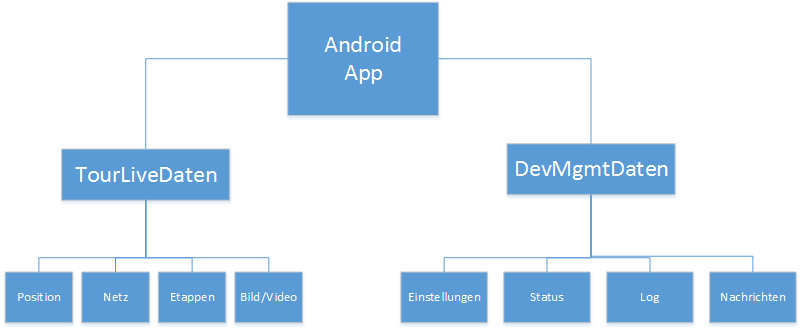
\includegraphics[width=120mm]{images/android/uebersicht.png}
	\caption{Grobstruktur der Android App}
	\label{fig:grobstrukturandroid} 
\end{figure}

\subsubsection{Schichtenmodell}
Die Android Applikation teilt sich in 3 Schichten auf.

\begin{figure}[H]
	\centering
	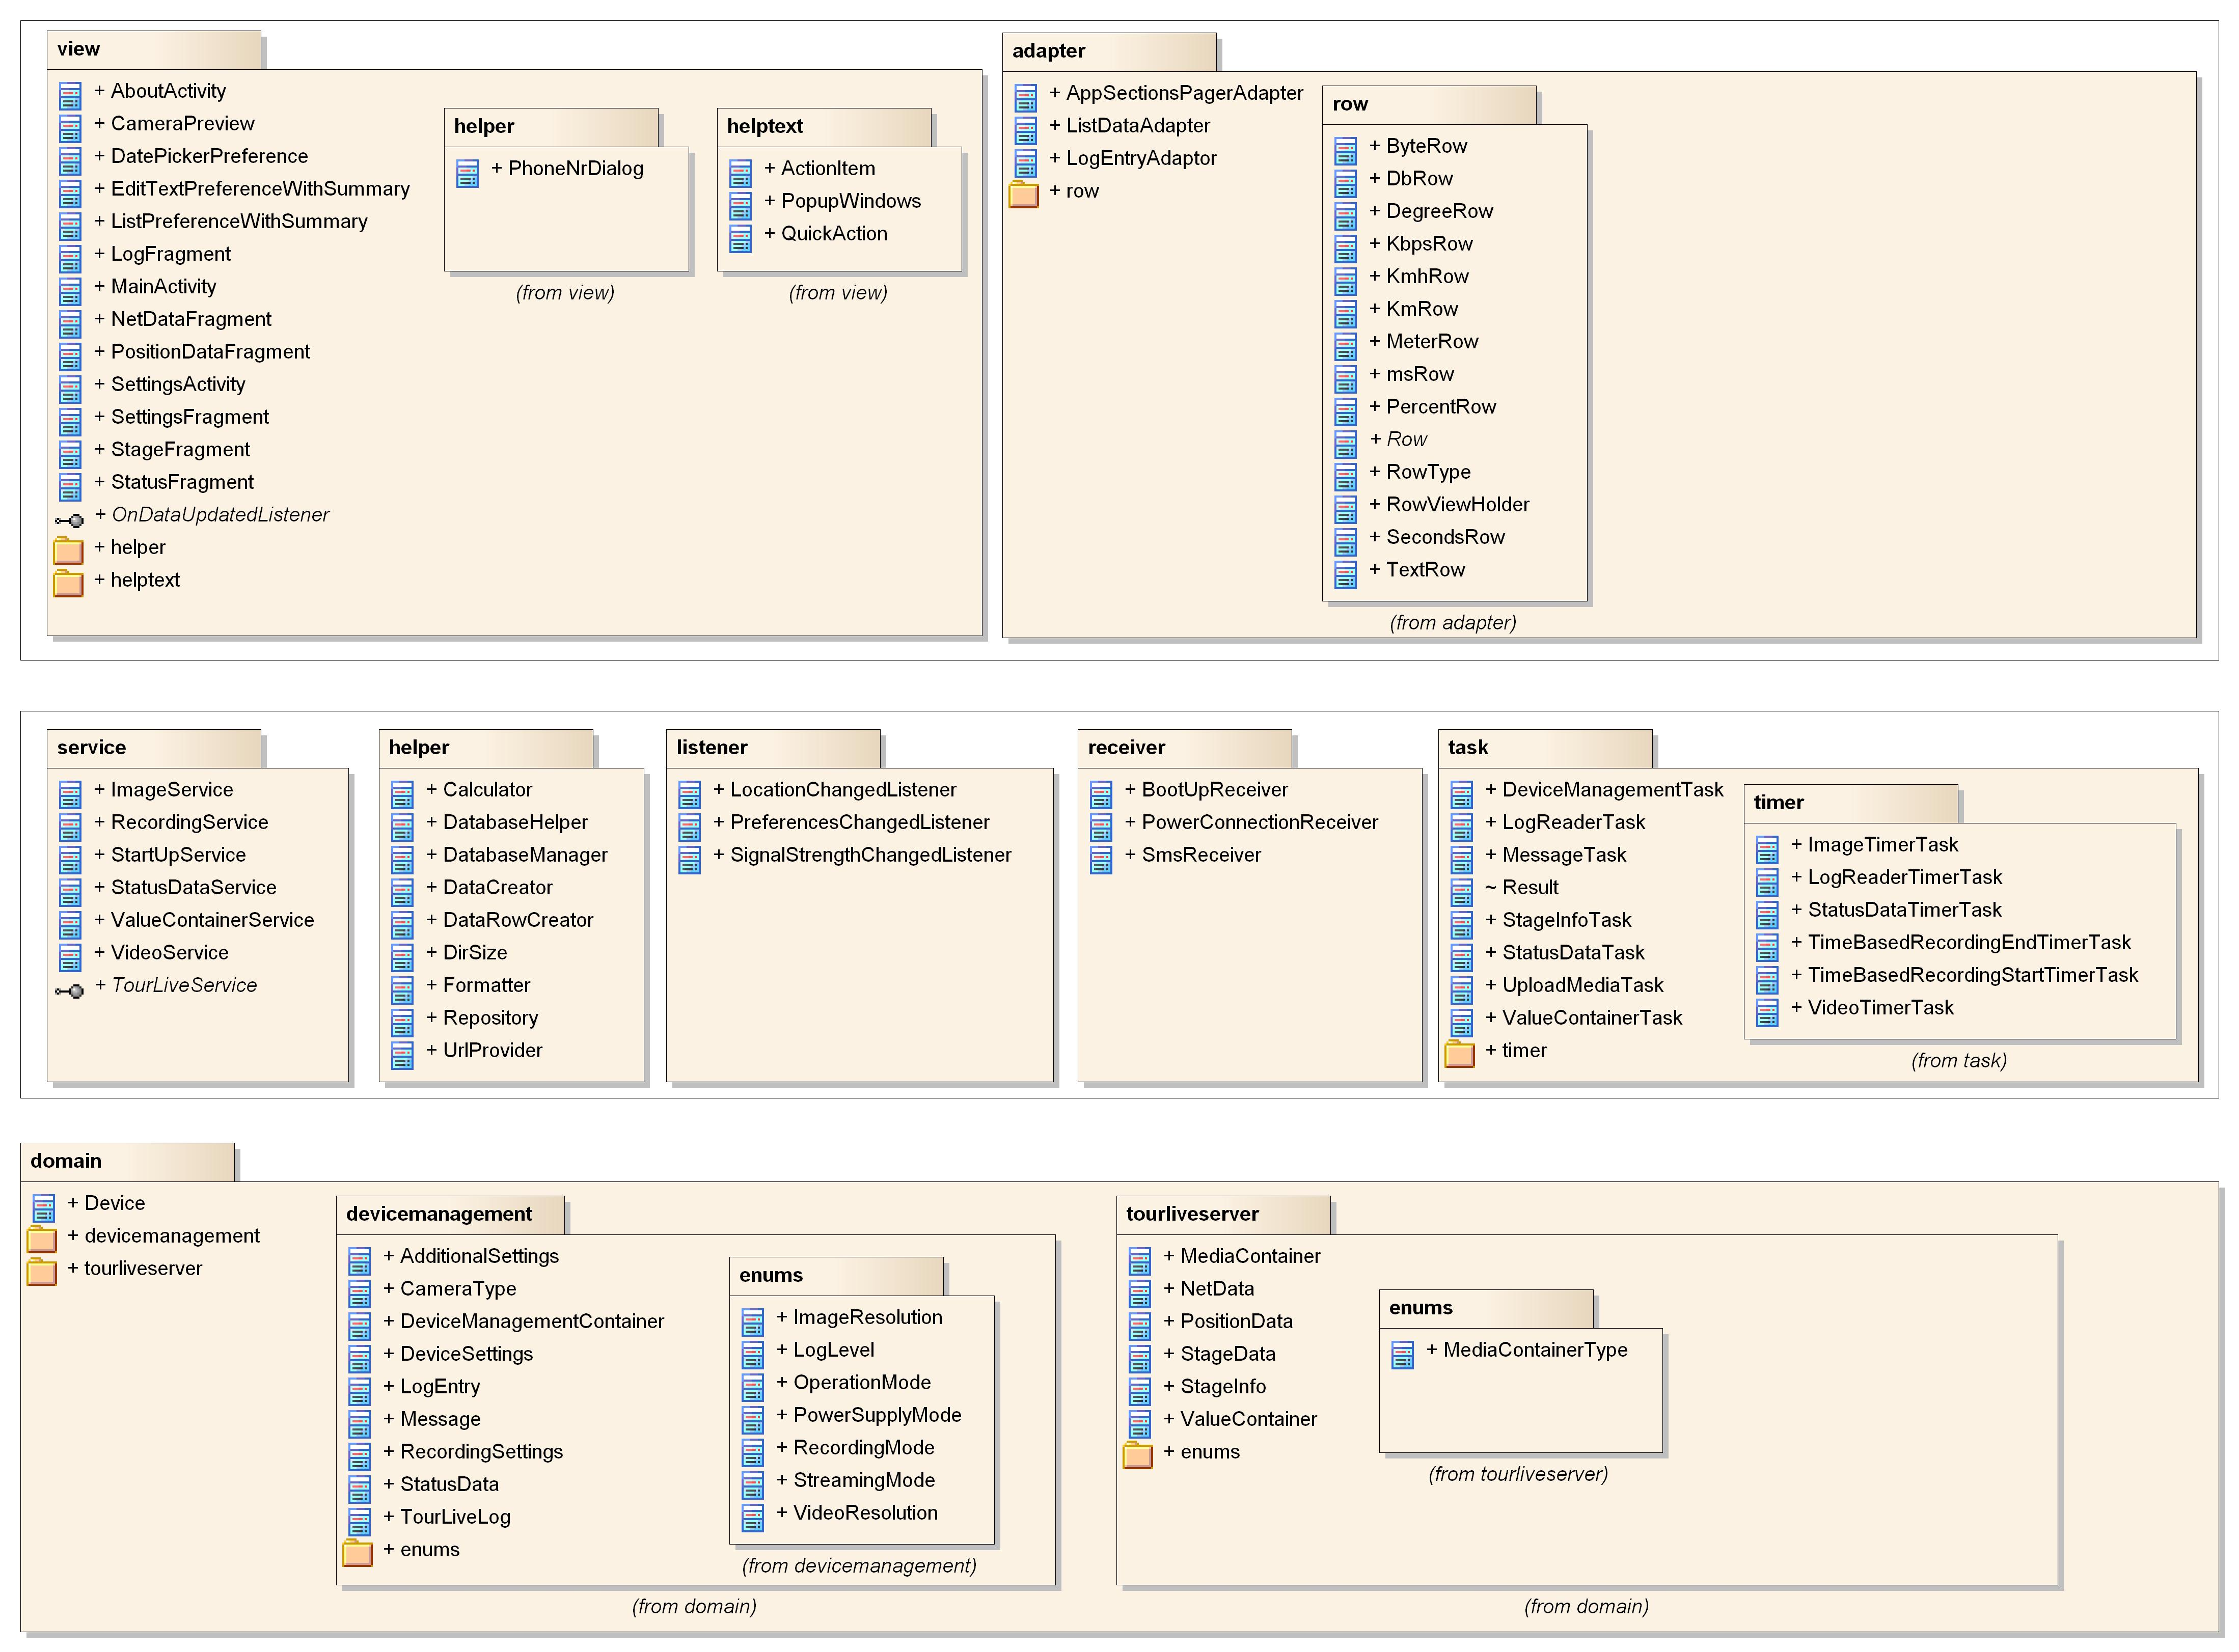
\includegraphics[width=150mm]{images/android/schichten.jpg}
	\caption{Packagediagramm des Aufnahmesystems}
\end{figure}

Die oberste Schicht stellt die Schnittstelle zum Benutzer dar. Diese Klassen in dieser Schicht sind für die Darstellung / Views zuständig. Die mittlere Schicht enthält die ganze Businesslogik. Dazu gehören Services, Timer, Listener, etc. Die unterste Schicht enthält die Domänenobjekte die die effektiven Daten (Positionsdaten, Konfigurationen, ...) enthalten. 

\subsubsection{Domain Model}
Das Domain Model des Aufnahmesystems setzt sich aus den Domain Models des TourLive Servers und des Device Management Servers zusammen. Im Aufnahmesystem kommen keine neuen Domänenobjekte hinzu.

\begin{figure}[H]
\centering
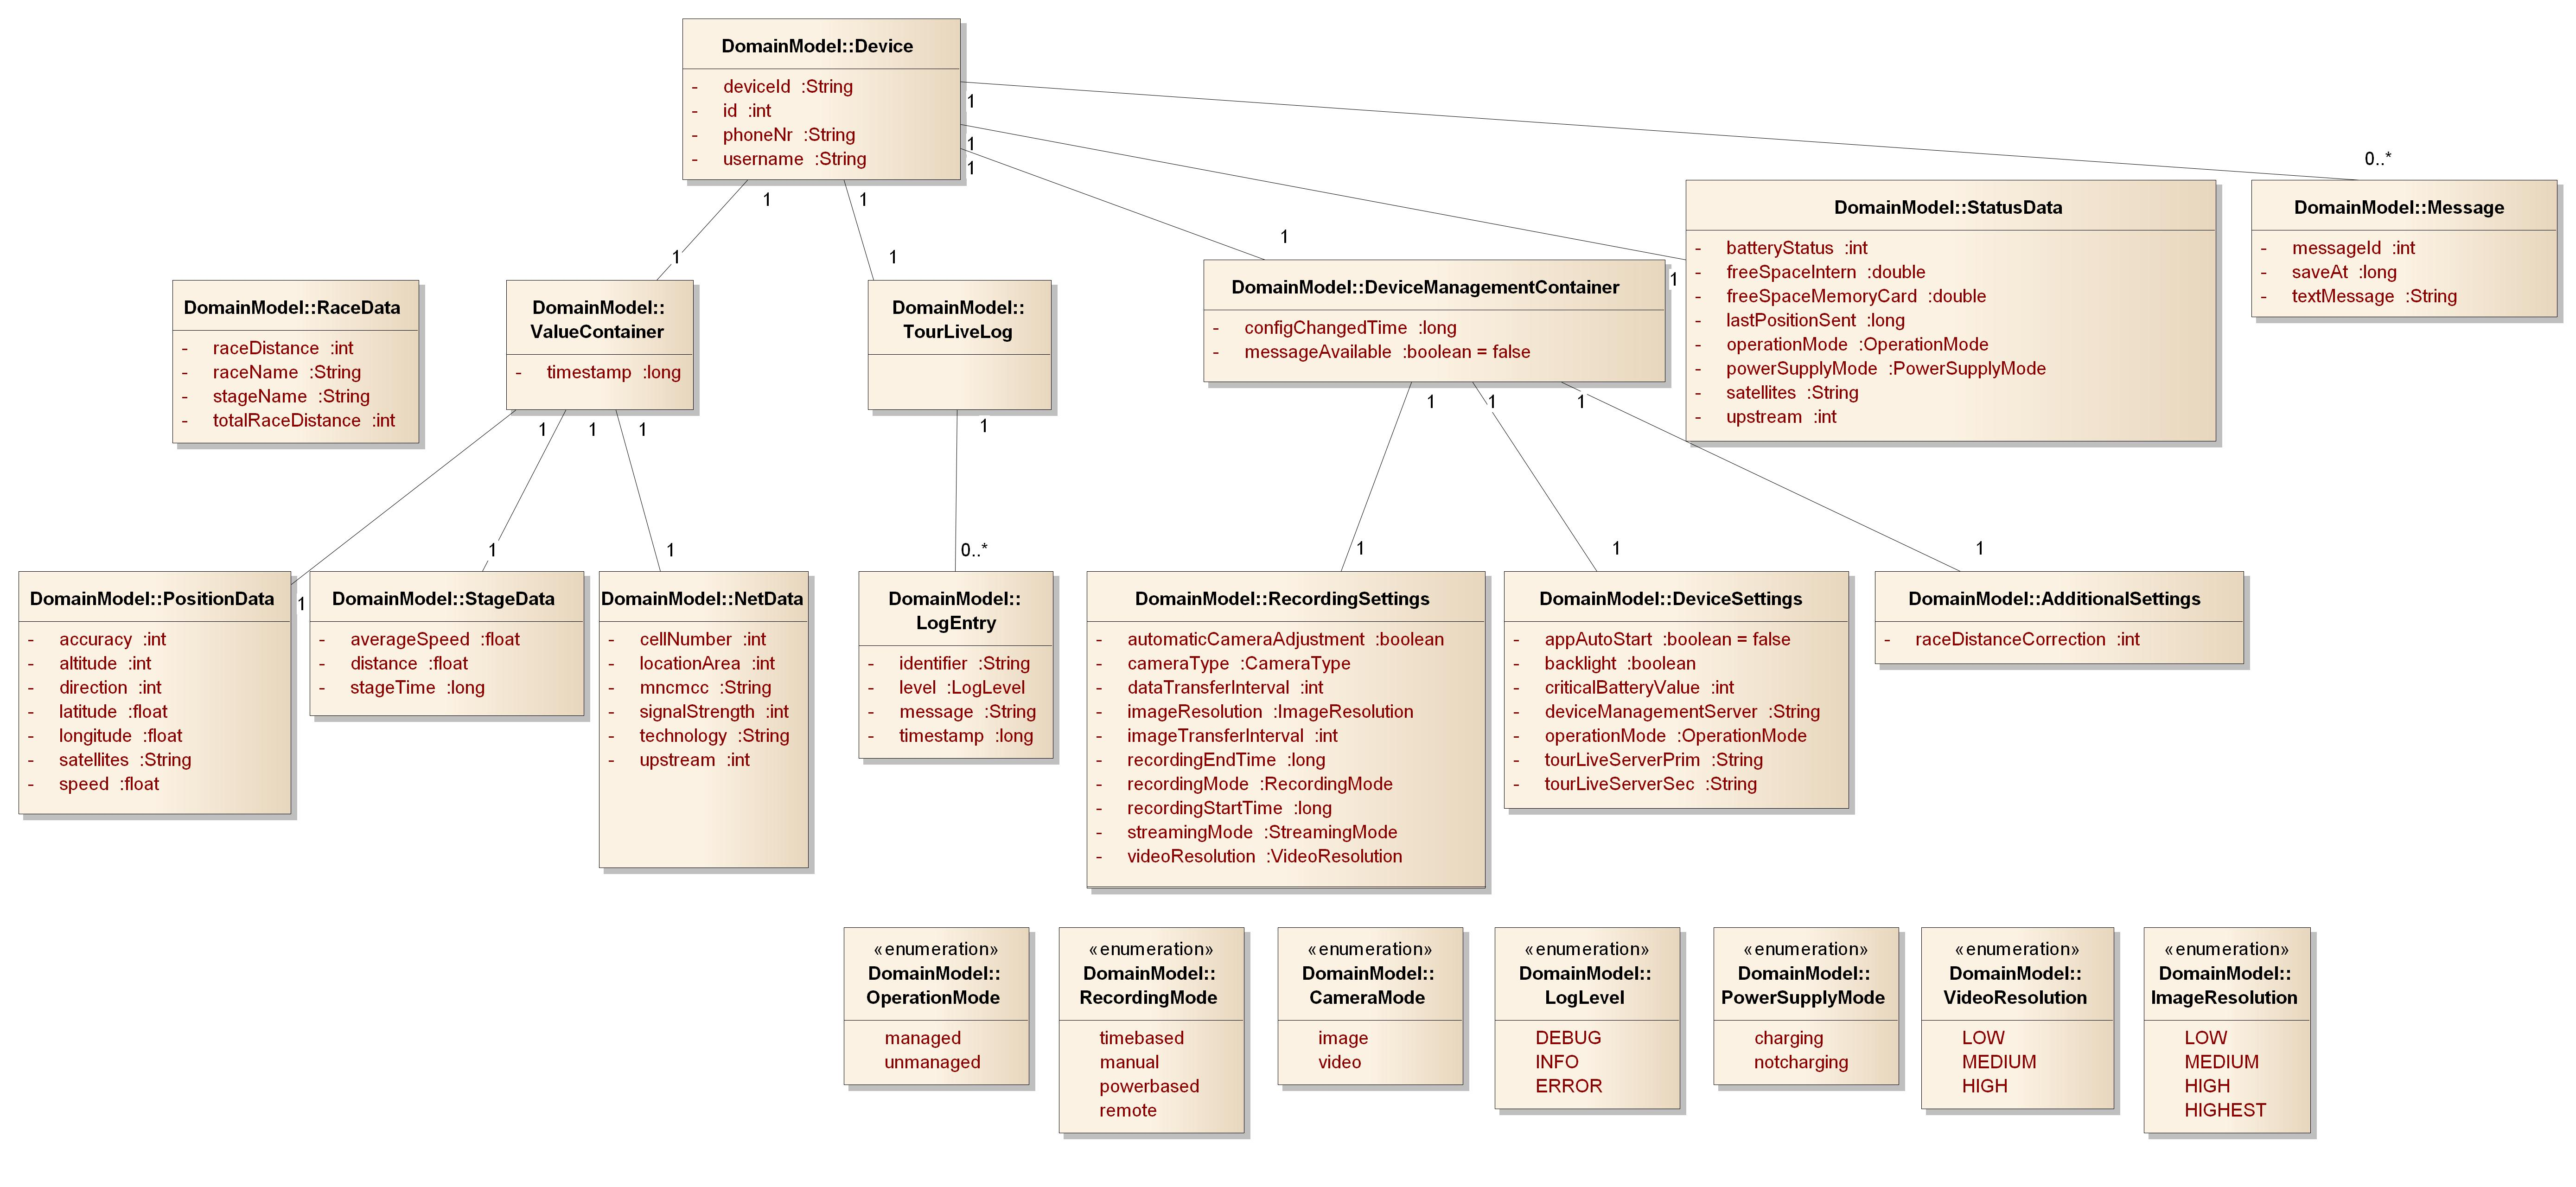
\includegraphics[width=150mm]{images/android/domainmodel.jpg}
\caption{Aufnahmesystem Domain Model}
\end{figure}

\subsubsection{Paketdiagramm}
Die TourLive Applikation hat folgende Paketstruktur. Als Grundstruktur wurde analog zum TourLive Server und dem Device Management Server \textit{ch.hsr.ba.tourlive} verwendet. Die TourLive Applikation verwendet zusätzlich die Subkategorie \textit{.android} sowie folgende applikationsspezifische Struktur:

\begin{longtable}{p{5.0cm} | p{7.1cm}}
\textbf{Paket} & \textbf{Inhalt} \\
\hline \hline 
. & enthält die initialisierende TourLiveApplication.java Klasse sowie Config.java \\ 
\hline 
.adapter & enthält Daten-Adapter um Listen darzustellen \\ 
\hline 
.adapter.row & enthält individuelle Listen Einträge \\ 
\hline 
.domain & enthält projektübergreifende Domain Klassen \\ 
\hline 
.domain.devmgmtsrv & enthält Device Management Server spezifische Domain Klassen \\ 
\hline 
.domain.devmgmtsrv.enums & enthält Device Management Service spezifische Enums \\ 
\hline 
.domain.tourliveserver & enthält TourLive Server spezifische Domain Klassen \\ 
\hline 
.domain.tourliveserver.enums & enthält TourLive Server spezifische Enums \\  
\hline 
.helper & enthält Hilfsklassen zur Berechnung von Werten \\ 
\hline 
.listener & enthält System Event-Listener \\ 
\hline 
.receiver & enthält Broadcast Receiver \\ 
\hline 
.service & enthält sämtliche Services \\ 
\hline 
.task & enthält sämtliche AsyncTasks \\ 
\hline 
.task.timer & enthält sämtliche TimerTasks \\ 
\hline 
.view & enthält Activities und Fragments \\ 
\hline 
.view.helper & enthält individuelle Dialoge \\ 
\hline 
.view.helptext & enthält die Hilfstext Klassen \\ 
\hline 
\end{longtable} 

\subsection{Architekturentscheide}

\subsubsection{Globaler Daten Provider - Repository.java}
Das Repository.java implementiert mit dem Singleton-Pattern fungiert als globaler Daten Provider und verhindert lange Aufrufketten. Das Repository bietet auf folgende Daten Zugriff:

\begin{itemize} [noitemsep,topsep=0pt]
	\item diverse Services
	\item das TourLiveLog
	\item Liste mit ValueContainers
	\item diverse globale Domänen Objekte
\end{itemize}

\subsubsection{Start der Applikation - TourLiveApplication.java}
Beim Start der TourLive Applikation müssen diverse Daten initialisiert werden. Um diese Initialisierung vor der ersten View durchzuführen wurde eine projektspezifische Klasse \textit{TourLiveApplication.java} geschrieben, die von der Android Klasse \textit{Application} ableitet. Eine von \textit{Application} abgeleitete Klasse darf nur einmalig vorkommen und wird als erste Klasse bei einem App-Start initialisiert.
\begin{quotation}
\textit{Base class for those who need to maintain global application state}.\footnote{Application class, \url{http://developer.android.com/reference/android/app/Application.html} besucht am: 10.04.2013}
\end{quotation}
Über die Klasse TourLiveApplication kann ausserdem auf den globalen Application-Context zugegriffen werden. Der zur Initialisierung diverser Objekte benötigt wird und wie folgt in den Android Developer Reference beschrieben ist.
\begin{quotation}
\textit{Interface to global information about an application environment. This is an abstract class whose implementation is provided by the Android system. It allows access to application-specific resources and classes, as well as up-calls for application-level operations such as launching activities, broadcasting and receiving intents, etc. }\footnote{Context class, \url{http://developer.android.com/reference/android/content/Context.html} besucht am: 13.04.2013}
\end{quotation}

\subsubsection{Caching der Daten}
Um einen lokalen Cache zu realisieren wird der auf SQLite basierende OR-Mapper ORMLite verwendet. Der Cache verhindert Datenverlust bei Applikationsabstürzen. In der SQLite-Datenbank werden folgende Objekte gespeichert:

\begin{itemize} [noitemsep,topsep=0pt]
	\item Bildinformationen (Binärdatei liegt im Dateisystem)
	\item Videoinformationen (Binrädatei leigt im Dateisystem)
	\item Positions-, Etappen- \& Netzdaten (ValueContainer)
	\item Geräteinformationen (Device)
	\item Log-Einträge
\end{itemize}

Um Objekte und ihre Attribute zu persistieren, werden diese in den Modelklassen mit Java Annotationen markiert. 

\subsubsection{Factory Pattern - DataCreator.java}
Das erstellen der ValueContainer, DeviceManagementContainer und anderen Datenstrukturen unterliegt einem relativ komplexen Vorgang, da unzählige Werte aus den verschiedensten Android Listener,  Android Provider und Android Services zusammengezogen werden müssen. Das Factory Pattern schafft Abbhilfe dies über ein einzelnes Objekt, den DataCreator, zu realisieren.

\subsubsection{Primärer / Sekundärer TourLive Server - URLProvider.java}
Eine Anforderung an das TourLive Aufnahmesystem ist die Implementation eines sekundären TourLive Servers der bei Ausfall des primären Servers die Daten empfangen und verarbeiten kann. Dies wurde über die Klasse URLProvider.java realisiert. Schlägt die Verbindung zum aktuell ausgewählten Server, in der Regel ist dies der primäre Server, mehrmals fehl, stellt der URLProvider den Zweitserver zur Verfügung. Die Anzahl möglicher Fehlschläge vor einem Wechsel ist in der Config.java definiert. Sämtliche genutzten URLs werden über den URLProvider bezogen.

\subsubsection{Unveränderbare Applikationskonfiguration - Config.java}
In der Config.java werden unveränderbare Applikationseinstellungen gespeichert. Diese sind direkt über public static final Attribute aufrufbar. Die Config.java enthält folgende Konfigurationen:
\begin{itemize} [noitemsep,topsep=0pt]
	\item sämtliche API-URLs des TourLive Servers und des Device Management Servers
	\item Speicherort im Dateisystem der Bilddateien
	\item Speicherort im Dateisystem der Videodateien
	\item Intervall wie oft der Gerätezustand dem Device Management Server übertragen werden soll
	\item Angaben zur Genauigkeit die eine GPS Location haben muss, damit sie nicht verworfen wird
\end{itemize}

\section{Realisierung}
Das Kapitel Realisation gibt Hinweise zur Umsetzung des TourLive Aufnahmesystems. Es werden interne Abläufe und Funktionen erläutert und bietet eine kurze Einführung wie das Ausnahmesystem funktioniert. 

\subsection{Grafische Oberfläche}
\subsubsection{Einführung in die grafische Oberfläche von Android}

Die grafische Oberfläche einer Android Applikation besteht in erster Linie aus Activities. Gemäss Android Developer Reference wird eine Activity wie folgt definiert.

\begin{quotation}
\textit{An activity is a single, focused thing that the user can do. Almost all activities interact with the user, so the Activity class takes care of creating a window for you in which you can place your UI.} \footnote{Activity, \url{http://developer.android.com/reference/android/app/Activity.html}, besucht am: 25.03.2013}
\end{quotation}

Die TourLive Applikation wurde mit folgenden drei Activities realisiert.
\begin{itemize} [noitemsep,topsep=0pt]
	\item MainActivity.java
	\item SettingsActivity.java
	\item AboutActivity.java
\end{itemize}

Zu einer Activity gehört jeweils eine *.java Datei sowie eine *.xml Datei die das Layout definiert. Innerhalb einer Activity wird mit Fragments gearbeitet, welche wie folgt definiert sind:

\begin{quotation}
\textit{A Fragment represents a behavior or a portion of user interface in an Activity.} \footnote{Fragment, \url{http://developer.android.com/reference/android/app/Fragment.html}, besucht am: 25.03.2013}
\end{quotation}

Fragments werden für die verschiedenen Tabs innerhalb der MainActivity verwendet wie nachfolgende Screenshots zeigen.

\subsubsection{Konkrete Umsetzung der grafischen Oberfläche}
Die \textit{MainActivity} bestehend aus MainActivity.java und main\_activity.xml ist die Hauptansicht der Applikation. Sie ist in drei Teile unterteilt, Header, Footer und Hauptbereich. Header und Footer sind in allen Tabs sichtbar.

\begin{figure}[H]
	\centering
	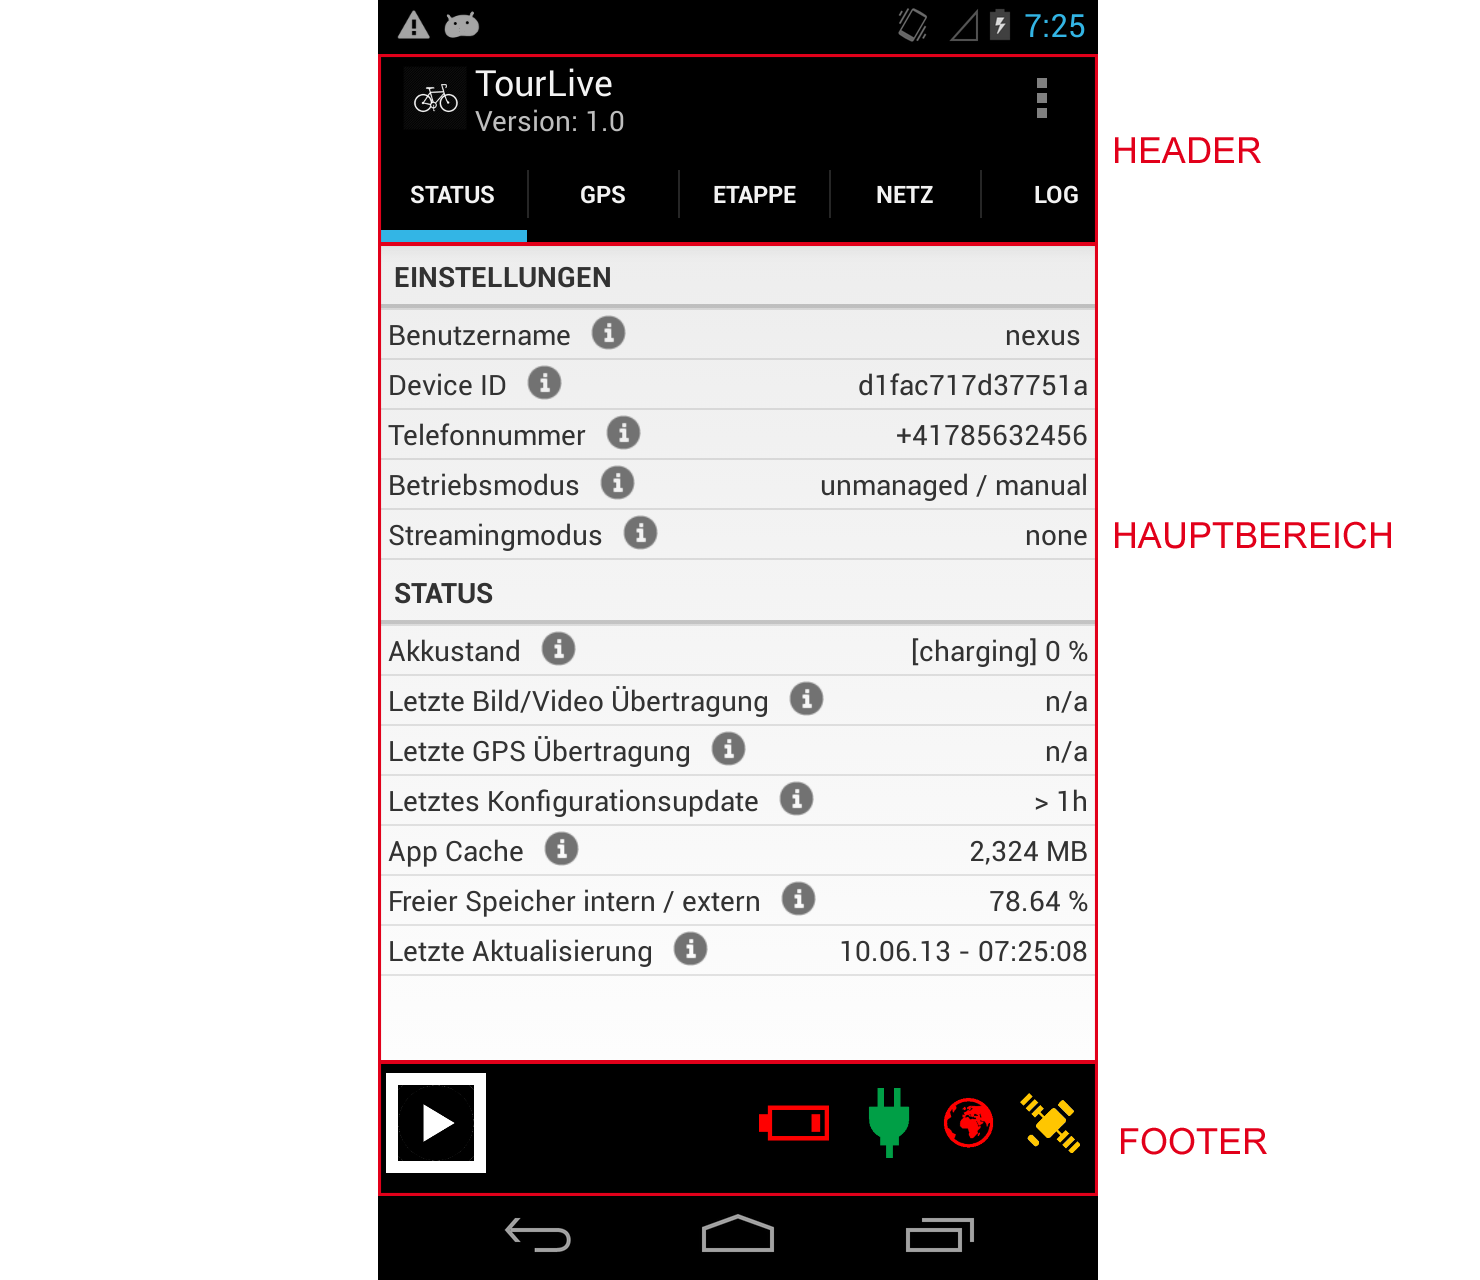
\includegraphics[width=120mm]{images/android/status.png}
	\caption{Aufnahmesystem MainActivity}
\end{figure}

\paragraph{Hauptbereich}
Der Inhalt des Hauptbereichs hängt vom selektierten Tab ab. Die einzelnen Ansichten Status, GPS, Etappe, Netz und Log wurden mit Fragments realisiert und basieren jeweils auf einer ListView.

\begin{quotation}
\textit{ListView is a view group that displays a list of scrollable items. The list items are automatically inserted to the list using an Adapter that pulls content from a source such as an array or database query and converts each item result into a view that's placed into the list.} \footnote{ListView, \url{http://developer.android.com/guide/topics/ui/layout/listview.html}, besucht am: 25.03.2013}
\end{quotation}

\paragraph{Header}
\begin{figure}[H]
	\centering
	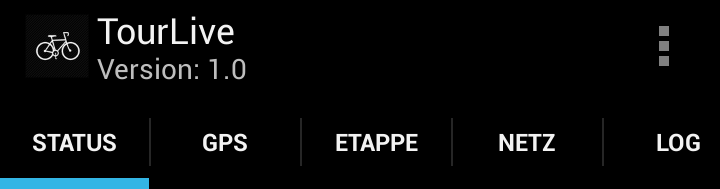
\includegraphics[width=60mm]{images/android/header.png}
	\caption{Aufnahmesystem Header}
\end{figure}
Der Header beinhaltet in der \textit{Action Bar} die aktuelle Versionsnummer, den Namen der Applikation sowie den Settings Button. Befindet sich die Applikation um Aufnahmemodus wird in roter Farbe der Text \textit{REC} eingeblendet. Unterhalb der \textit{Action Bar} befindet sich die \textit{Top Bar}, in der die verschiedenen Tabs angezeigt werden. Innerhalb des Content Bereiches kann mit einem Swipe zwischen den verschiedenen Views  hin und hergewechselt werden.

\paragraph{Settings Button}
Über den Settings Button wird folgendes Menü eingeblendet. Befindet sich die Applikation im Aufnahmemodus ist der Menüeintrag \textit{Einstellungen} deaktiviert. Die restlichen Aktionen sind trotzdem Verfügbar.

\begin{figure}[H]
	\centering
	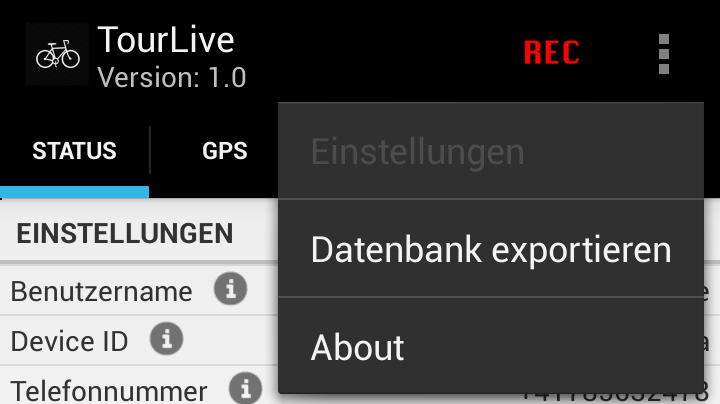
\includegraphics[width=60mm]{images/android/settingsclicked.png}
	\caption{Aufnahmesystem Settings Button Clicked}
\end{figure}



\paragraph{Footer}
\begin{figure}[H]
	\centering
	
\includegraphics[width=60mm]{images/android/footer.png}
	\caption{Aufnahmesystem Footer}
\end{figure}
Der Footer zeigt den Status der App. Die Symbole werden je nach Gesundheitszustand der Applikation rot, gelb oder in grün dargestellt. Welche Farben welchem Gesundheitszustand entspricht, ist in den Anforderungen im Anhang im Kapitel \ref{par:alarming} beschrieben.\\

Mit dem Recording Button links kann die Aufnahme gestartet und gestoppt werden. Der Button ist nur aktiviert, wenn der Aufnahmemodus auf Manuell gesetzt ist.

\paragraph{Einstellungen}
\begin{figure}[H]
	\centering
	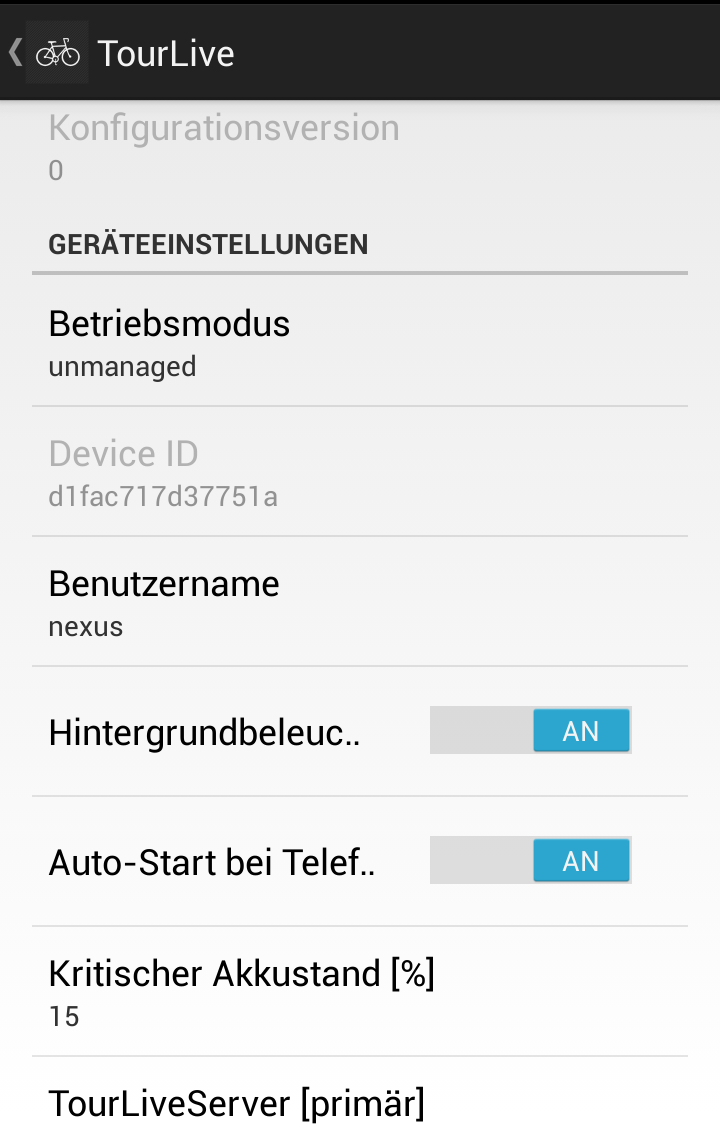
\includegraphics[width=60mm]{images/android/settings.png}
	\caption{Aufnahmesystem Einstellungen}
\end{figure}

Der oben abgebildete Screenshot zeigt einen Ausschnitt der Aufnahmesystemeinstellungen. Sämtliche Einstellungen können auch am Device Management Server verwaltet werden und werden regelmässig synchronisiert. Folgende Einstellungen sind möglich:

\begin{itemize}
	\item Konfigurationsversion (read-only)
	\item Betriebsmodus (managed / unmanaged)
	\item Device ID (read-only)
	\item Benutername (String)
	\item Hintergrundbeleichtung (on / off)
	\item Auto-Start bei Gerätestart (on / off)
	\item Kritischer Akku-Stand (0 - 100 \%)
	\item TourLive Server primär (String)
	\item TourLive Server sekundär (String)
	\item Device Management Server primär (String)
	\item Aufnamemodus (manuell, strombasiert, ferngesteuert, zeitbasiert)
	\item Startzeit (DateTimePicker - nur bei Aufnahmemodus zeitbasiert)
	\item Endzeit (DateTimePicker - nur bei Aufnahmemodus zeitbasiert)
	\item Datenübertragunsintervall (Integer)
	\item Kamera automatisch ausrichten (on / off)
	\item Kamera (front / back)
	\item Streamingmodus (Bilder / Videos / Nichts)
	\item Bildauflösung (320x240, 640x480, 1280x960, 1600x1200)
	\item Bildübertragunsintervall (Integer)
	\item Videoauflösung (176x144, 720x480, 1280x720)
	\item Renndistanzkorrektur (Integer)
\end{itemize}
Es ist ausserdem möglich sämtliche lokal gespeicherten Etappen und Positionsdaten zu löschen, sämtliche Bilder und Videodaten zu löschen und die Telefonnummer beim Wechsel der SIM-Karte anzupassen.

\subsection{Berechtigungen}
Das Starten einer Android Applikation erfordert je nach Funktionalität der Applikation bestimmte Systemberechtigungen, die bei der Installation \textit{Akzeptiert} werden müssen.
\begin{figure}[H]
	\centering
	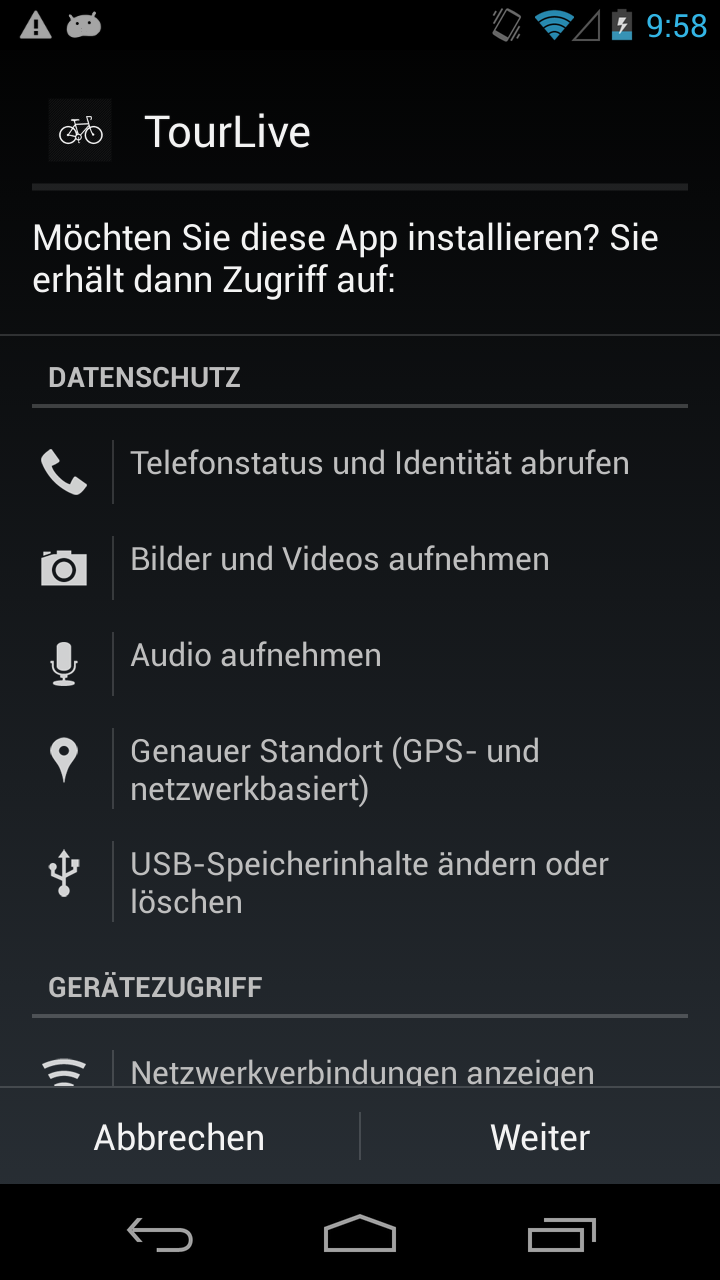
\includegraphics[width=60mm]{images/android/berechtigungen.png}
	\caption{Aufnahmesystem Berechtigungen}
\end{figure}
\subsubsection{Datenschutz}

\begin{itemize} [noitemsep,topsep=0pt]
	\item \textbf{Telefonstatus und Identität abrufen:} Berechtigt das auslesen der Telefonnummer
	\item \textbf{Bilder und Videos aufnehmen:} Berechtigt die Aufnahme von Bildens und Videos
	\item \textbf{Audio aufnehmen:} Berechtigt die Aufnahme von Audio
	\item \textbf{Genauer Standort:} Berechtigt die Nutzung des GPS Providers
	\item \textbf{USB Speicherinhalte ändern und löschen:} Berechtigt den Zugriff auf das Dateisystem (Bilder und Videos)
\end{itemize}

\subsubsection{Gerätezugriff}
\begin{itemize} [noitemsep,topsep=0pt]
	\item \textbf{Netzwerkverbindungen:} Berechtigt zur Nutzung des mobilen Netzwerks
	\item \textbf{Beim Start ausführen:} Berechtigt die Nutzung des Auto-Starts
	\item \textbf{Zugriff auf geschützten Speicher testen:} Berechtigt den Zugriff auf das Dateisystem (SQLite)
\end{itemize}

\subsection{I18N}
Die Applikation ist in deutscher sowie englischer Sprache verfügbar. Weitere Sprachen lassen sich einfach durch erstellen  und übersetzen der Ordnerstruktur TourLive/res/values-SPRACHE hinzufügen.

\subsection{Services, Tasks \& TimerTasks}
Die TourLive Applikation arbeitet mit mehreren Services. Diese implementieren in der Regel das eigens für diese Applikation entworfene Interface \textit{TourLiveService.java}. Die Services werden meistens in Verbindung mit einem \textit{Timer} genutzt der wiederum einen \textit{TimerTask} voraussetzt.

\begin{quotation}
\textit{Each timer has one thread on which tasks are executed sequentially. When this thread is busy running a task, runnable tasks may be subject to delays.} \footnote{Timer, \url{http://developer.android.com/reference/java/util/Timer.html}, besucht am: 11.04.2013}
\end{quotation}

\begin{quotation}
\textit{The TimerTask class represents a task to run at a specified time. The task may be run once or repeatedly.} \footnote{TimerTask, \url{http://developer.android.com/reference/java/util/TimerTask.html}, besucht am: 11.04.2013}
\end{quotation}

Folgende Services, Timer und TimerTask werden in der TourLive Applikation verwendet.
\subsubsection{RecordingService} 
\textit{RecordingService.java} ist verantwortlich für die Aufnahme von Live Informationen. Wird entweder manuell über den Start-Button, via Device Management Server über den fernstart, strom- oder zeitbasiert gestartet. Direkt mit dem RecordingService verknüpft sind folgende Services: ValueContainerService, ImageService und der VideoService.
\subsubsection{ValueContainerService} 
\textit{ValueContainerService.java} ist für die Übertragung von Positionsdaten (ValueContainer) verantwortlich. Der ValueContainerService registriert einen LocationListener der GPS-Updates meldet und diese dann mit Hilfe des DataCreators in ValueContainer-Objekt erstellt und per ValueContainerTask an den TourLive Server überträgt.
\subsubsection{ImageService} 
\textit{ImageService.java} ist für die Übertragung von Bilddaten verantwortlich. Der ImageService terminiert mit der Unterstützung eines Timers den TimerTask \textit{ImageTimerTask.java} der in regelmässigem Intervall ein Einzelbild aufnimmt und dieses per \textit{UploadMediaTask.java} an den TourLive Server sendet. 
\subsubsection{VideoService} 
\textit{VideoService.java} ist für die  Übertragung von Videodaten verantwortlich. Analog zum ImageServer nutzt der VideoService den \textit{VideoTimerTask.java} zur Aufnahme von Videosequenzen und den gemeinsamen UploadMediaTask.java zur Übertragung der Videosequenzen an den TourLive Server.
\subsubsection{StartUpService} 
\textit{StartUpService.java} ist für den Auto-Start der Applikation nach dem Gerätestart verantwortlich, sofern dieser in den Einstellungen aktiviert ist.
\subsubsection{StatusDataService} 
\textit{StatusDataService.java} ist für die  Übertragung des Gerätezustandes verantwortlich. Mit Hilfe eines Timers und des \textit{StatusDataTimerTask.java} wird in regelmässigem Intervall der Gerätezustand an den Device Management Server übertragen.

\subsection{Kommunikation mit den Servern}
Für die Übertragung der Daten an die beiden Server wurden AsyncTasks verwendet. Diese ermöglichen eine einfache Anwendung von Threads und sind in der Android Developer Reference wie folgt definiert: 

\begin{quotation}
\textit{AsyncTask enables proper and easy use of the UI thread. This class allows to perform background operations and publish results on the UI thread without having to manipulate threads and/or handlers. An asynchronous task is defined by a computation that runs on a background thread and whose result is published on the UI thread. An asynchronous task is defined by 3 generic types, called Params, Progress and Result, and 4 steps, called onPreExecute, doInBackground, onProgressUpdate and onPostExecute.} \footnote{AsyncTask, \url{http://developer.android.com/reference/android/os/AsyncTask.html}, besucht am: 13.04.2013}
\end{quotation}

Es folgt eine kurze Auflistung der implementieren AsyncTasks.
\begin{itemize} [noitemsep,topsep=0pt]
	\item \textit{DeviceManagementTask.java} überträgt die Einstellungen an den Device Management Server und registriert das Gerät beim Applikationsstart.
	\item \textit{LogReaderTask.java} aktualisiert die LogView in alle 5 Sekunden.
	\item \textit{MessageTask.java} bezieht Nachrichten vom Device Management Server, sofern welche vorhanden sind
	\item \textit{StageInfoTask.java} bezieht Renn- und Etappeninformationen vom TourLive Server
	\item \textit{StatusDataTask.java} sendet den Gerätezustand an den Device Management Server und empfängt allfällige Konfigurationsänderungen vom Device Management Server. 
	\item \textit{UploadMediaTask.java} sendet Bild- und Videodaten an den TourLive Server
	\item \textit{ValueContainerTask.java} sendet Positionsdaten an den TourLive Server
\end{itemize}

\subsection{Listener \& BroadcastReceiver}
Listener und BroadcastReceiver empfangen System- und andere Events. 
\begin{itemize} [noitemsep,topsep=0pt]
	\item \textit{LocationChangedListener.java} meldet Positionsupdates.
	\item \textit{PreferenceChangedListener.java} meldet Einstellungsänderungen.
	\item \textit{SignalStrengthListener.java} meldet Signalstärkenänderungen.
	\item \textit{BootUpReceiver.java} meldet einen Gerätestart.
	\item \textit{PowerConnectionReceiver.java} meldet Änderungen in der Stromversorgung.
\end{itemize}

\subsection{Aufnahme von Bildern und Videosequenzen}
Die Aufnahme von Bild- und Videosequenzen kann über die Android API grundsätzlich ziemlich komfortabel realisiert werden. Vorausgesetzt wird lediglich eine View (Bereich auf dem Bildschirm) die als Kamera Vorschau genutzt werden kann. 

\begin{quotation}
\textit{Sets the Surface to be used for live preview. Either a surface or surface texture is necessary for preview, and preview is necessary to take pictures.} \footnote{AsyncTask, \url{http://developer.android.com/reference/android/hardware/Camera.html\#setPreviewDisplay\%28android.view.SurfaceHolder\%29}, besucht am: 17.04.2013}
\end{quotation}

Eine View wiederum muss mit einer Activity verknüpft werden und eine Activity wiederum kennt verschiedene Status (\textit{active}, \textit{paused}, \textit{stopped}, \textit{destroyed}). Welche Activity sich in welchem Status befindet wird vom Android Betriebssystem verwaltet. Grundsätzlich kann aber davon ausgegangen werden, dass eine Activity sich nicht mehr im Status \textit{active} befindet, wenn die Applikation sich im Hintergrund befindet oder der Bildschirm sich abdunkelt. Befindet sich eine Activity nicht mehr im Status \textit{active} kommt es vor, dass der Garbage Collector View-Objekte aufräumt die beim reaktivieren der Activity neu initialisiert werden.
\\

Mit diesem Verhalten der Android API gibt es zwei Konflikte mit den Anforderungen an die TourLive Applikation. 

Das erste Problem mit der geforderten View die als Vorschau benötigt wird,  kann mit einer 1x1 Pixel grossen View die "unsichtbar" in einer Ecke angezeigt wird, gelöst werden. 

Das zweite, etwas grössere Problem besteht darin, dass Bilder und Videosequenzen auch aufgenommen werden sollen wenn die Applikation im Hintergrund oder mit abgedunkelten Bildschirm läuft. Da in diesem beiden Fällen die Möglichkeit besteht, dass die MainActivity in einen anderen Status als \textit{active} wechselt, kann es vorkommen, dass die View für die Kamera Vorschau vom Garbage Collector aufgeräumt wird. In diesem Fall muss die MainActivity neu gestartet und die View für die Kamera Vorschau neu initialisiert werden. 

Da die Android Kamera Design Prinzipien nicht für einen solchen Verwendungszweck ausgelegt ist (Aufnahme ohne Vorschau, Aufnahme bei abgedunkeltem Bildschirm / Applikation im Hintergrund) kann es während dem Betrieb zu unvorhergesehenen Problemen (Exceptions) kommen.

\subsection{Datenbank}
Für das lokale Caching werden Daten mittels ORMLite in die Datenbank geschrieben. Eine Klasse wird mittels Annotation als Datenbankklasse erkannt.

\begin{lstlisting}[language=Java, caption=ORMLite Annotations]
@DatabaseTable
public class Device {
	@JsonIgnore
	@DatabaseField(generatedId = true)
	private int id;
	@DatabaseField
	private String deviceId;
	@DatabaseField
	private String username;
	@DatabaseField
	private String phoneNr;
}
\end{lstlisting}

\begin{itemize}
\item \textbf{\textit{@DatabaseTable}:} mit dieser Annotation wird angegeben, dass die annotierte Klasse  eine gemappte Datenbank Klasse ist.
\item \textbf{\textit{@DatabaseField}:} das folgende Attribut ist eine Spalte in der Datenbank. Mittels generatedID = true wird für das Attribut eine eindeutige ID generiert.
\end{itemize}


Die Klasse \textit{DatabaseHelper.java} verwaltet die Zugriffe auf die Datenbank. Beim ersten Start der App werden die Tabellen generiert. Werden später neue Attribute hinzugefügt, so muss die Datenbankversion erhöht und in der \textit{onUpgrade} - Methode ein Update-Script zur Verfügung gestellt werden.\\

Der \textit{DatenbankManager.java}, eine Singleton Klasse, ermöglicht den Zugriff über den \textit{DatabaseHelper.java} auf die Datenbank. Im \textit{DatenbankManager.java} sind sämtliche \textit{\gls{CRUD}}-Operationen enthalten.

\subsection{Systemsequenzdiagramme}
Dieses Kapitel beschreibt die Abläufe innerhalb der Applikation in Form von Systemsequenzdiagrammen. Sie geben eine grobe Übersicht wie die bisher erwähnten Klassen zusammenarbeiten.

\subsubsection{Applikation im Ruhezustand}
Folgendes Diagramm beschreibt die Applikation im Ruhezustand. In regelmässigem Intervall (wird in der \textit{Config.java} definiert.) wird der Gesundheitszustand des Gerätes an den Device Management Server übertragen. Der Device Management Server antwortet mit der gespeicherten Gerätekonfiguration des Gerätes sowie einem Message-Flag, dass kennzeichnet wenn eine Nachricht für das Gerät vorhanden ist. 

Sind keine Renn- und Etappeninformationen vorhanden oder sind diese veraltet, werden diese nach Beendigung des ersten Requests beim TourLive Server abgerufen.

Wurde zudem das Message-Flag gesetzt, wird in einem weiteren Request die Nachricht abgerufen. 

 
\begin{figure}[H]
	\centering
	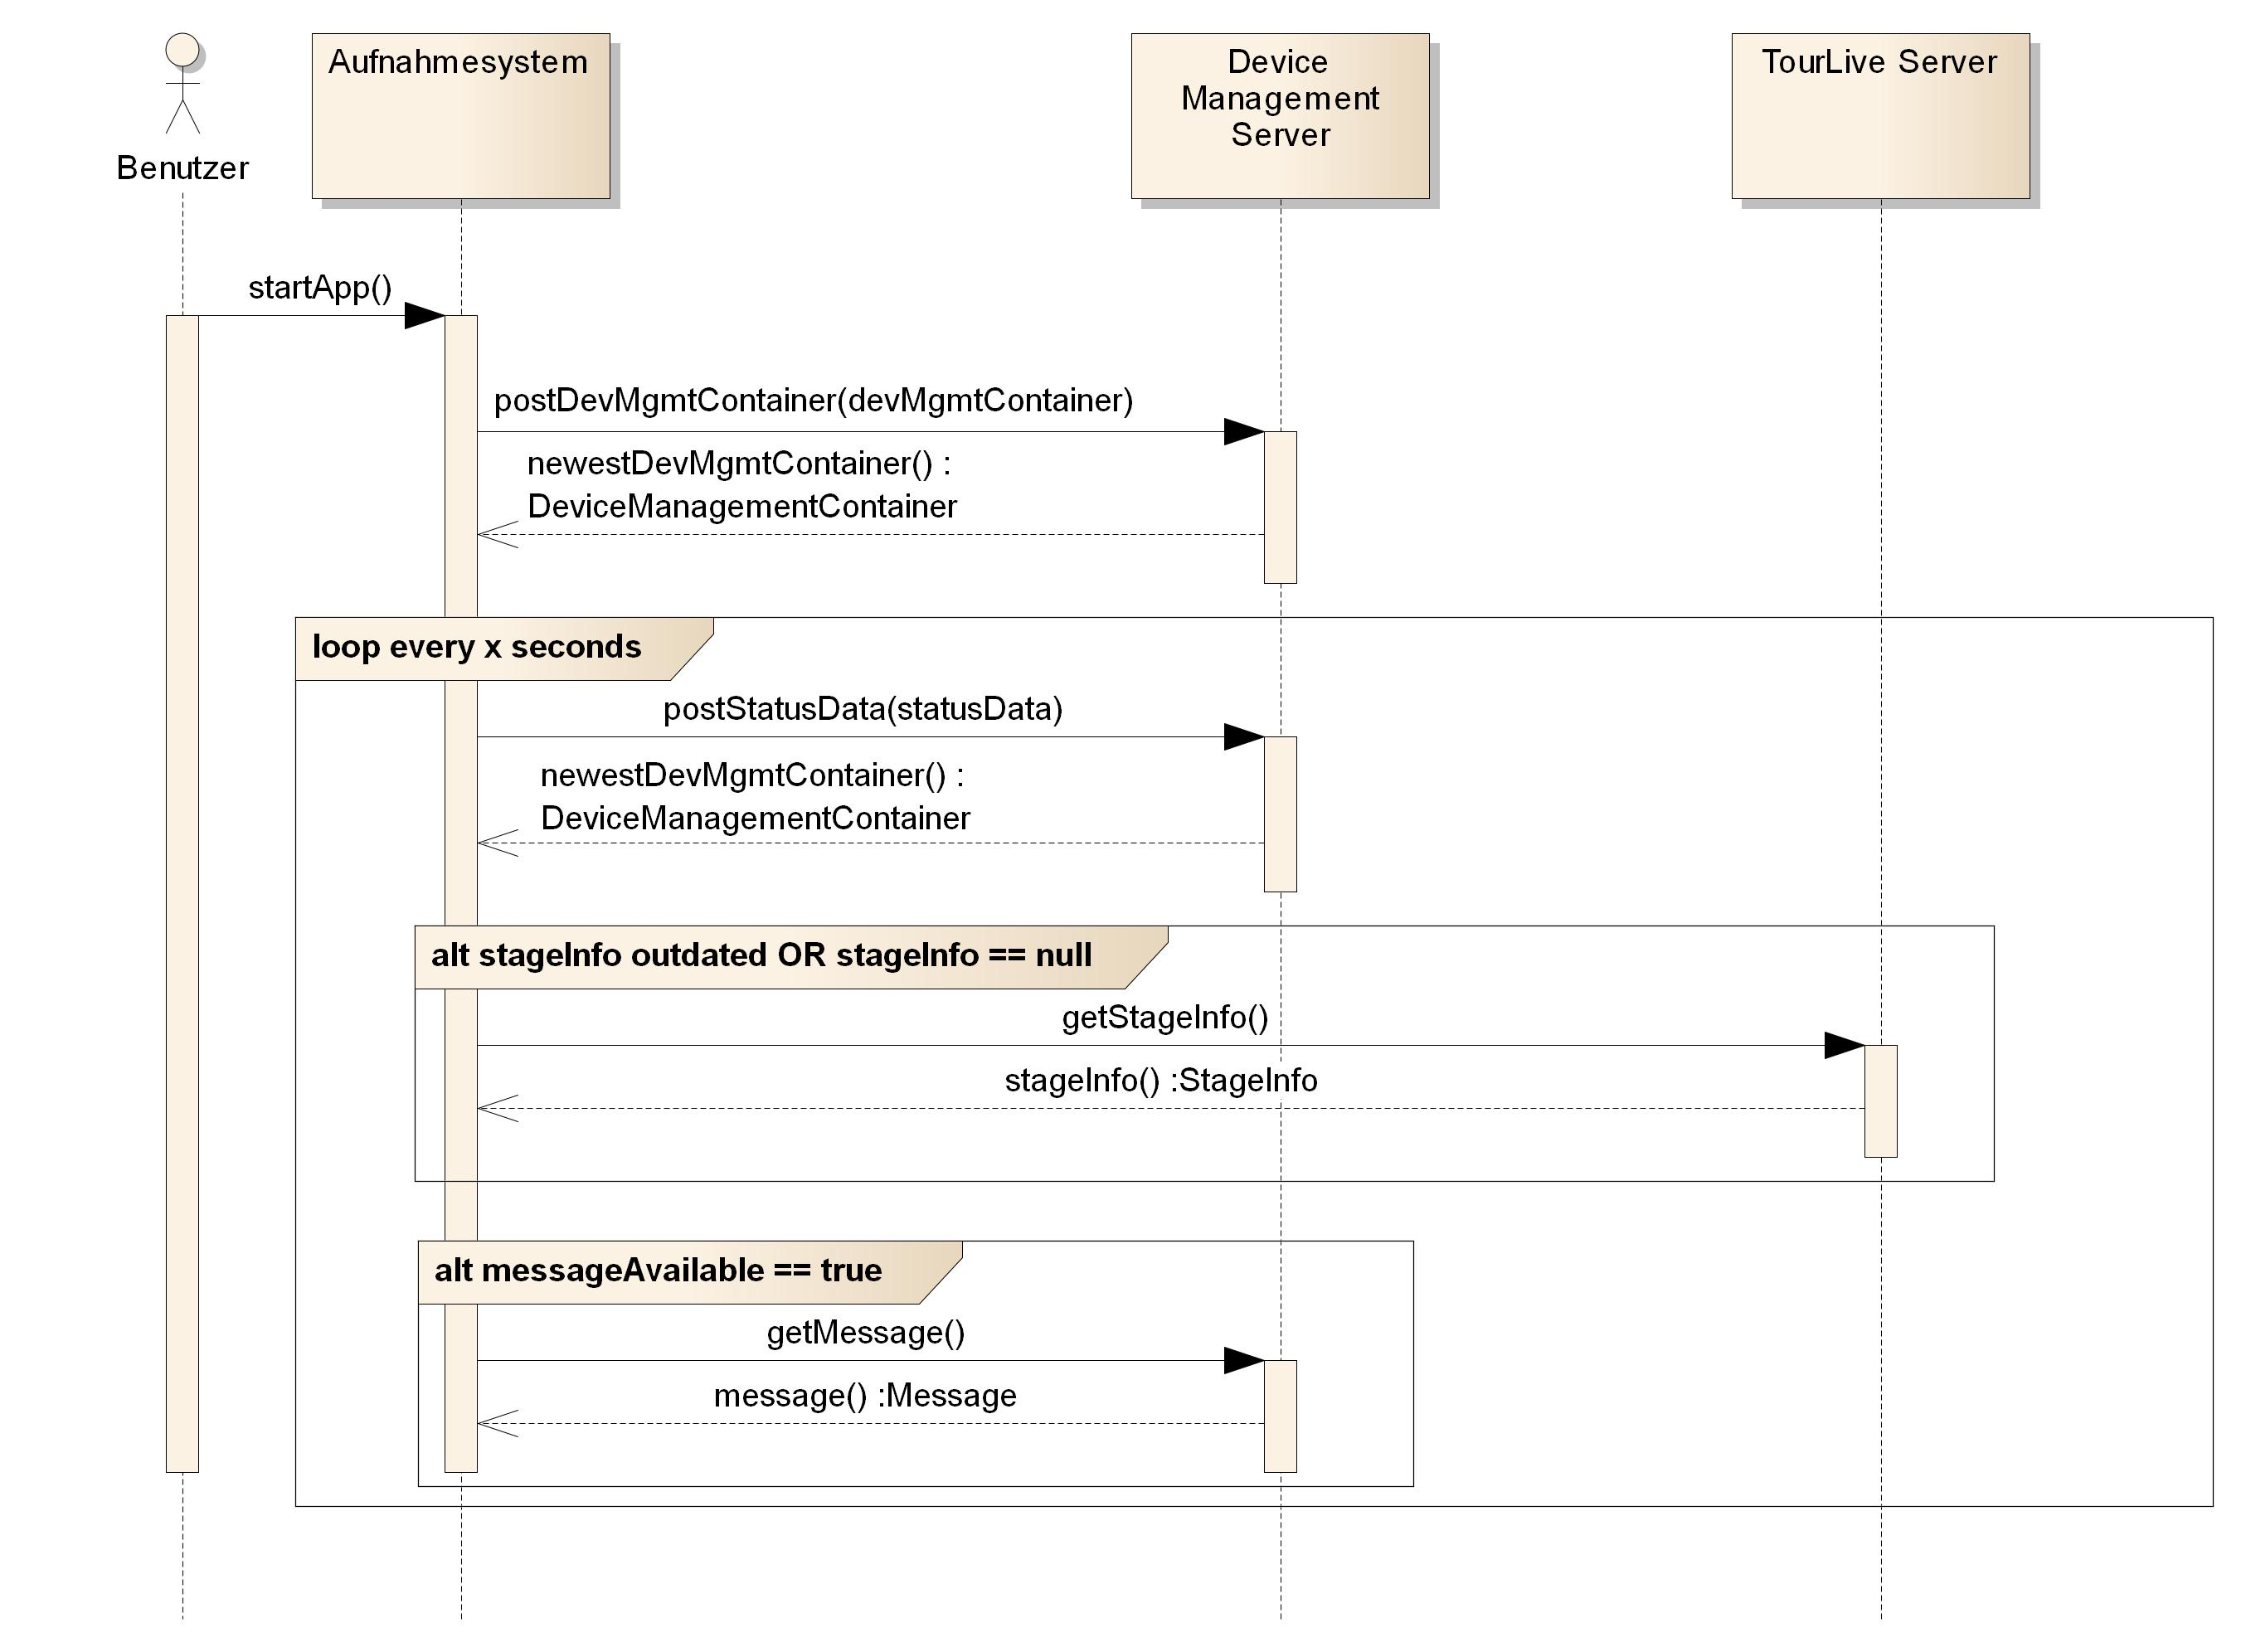
\includegraphics[width=150mm]{images/android/permanent_taskes.jpg}
	\caption{Aufnahmesystem Permanente Tasks}
\end{figure}

\pagebreak
\subsubsection{Applikation im Aufnahemodus}
Folgendes Diagramm zeigt die Abläufe beim Starten des Aufnahmemodus (\textit{RecordingService.java}). Die Operation \textit{startRecording()} entspricht dem \textit{RecordingService.java}. Der Start des RecordingServices beinhaltet auf jeden Fall den Start des  \textit{ValueContainerService.java}. Je nach Konfiguration wird zudem der \textit{VideoService.java}, der \textit{ImageService.java} oder keiner der beiden gestartet.

\begin{figure}[H]
	\centering
	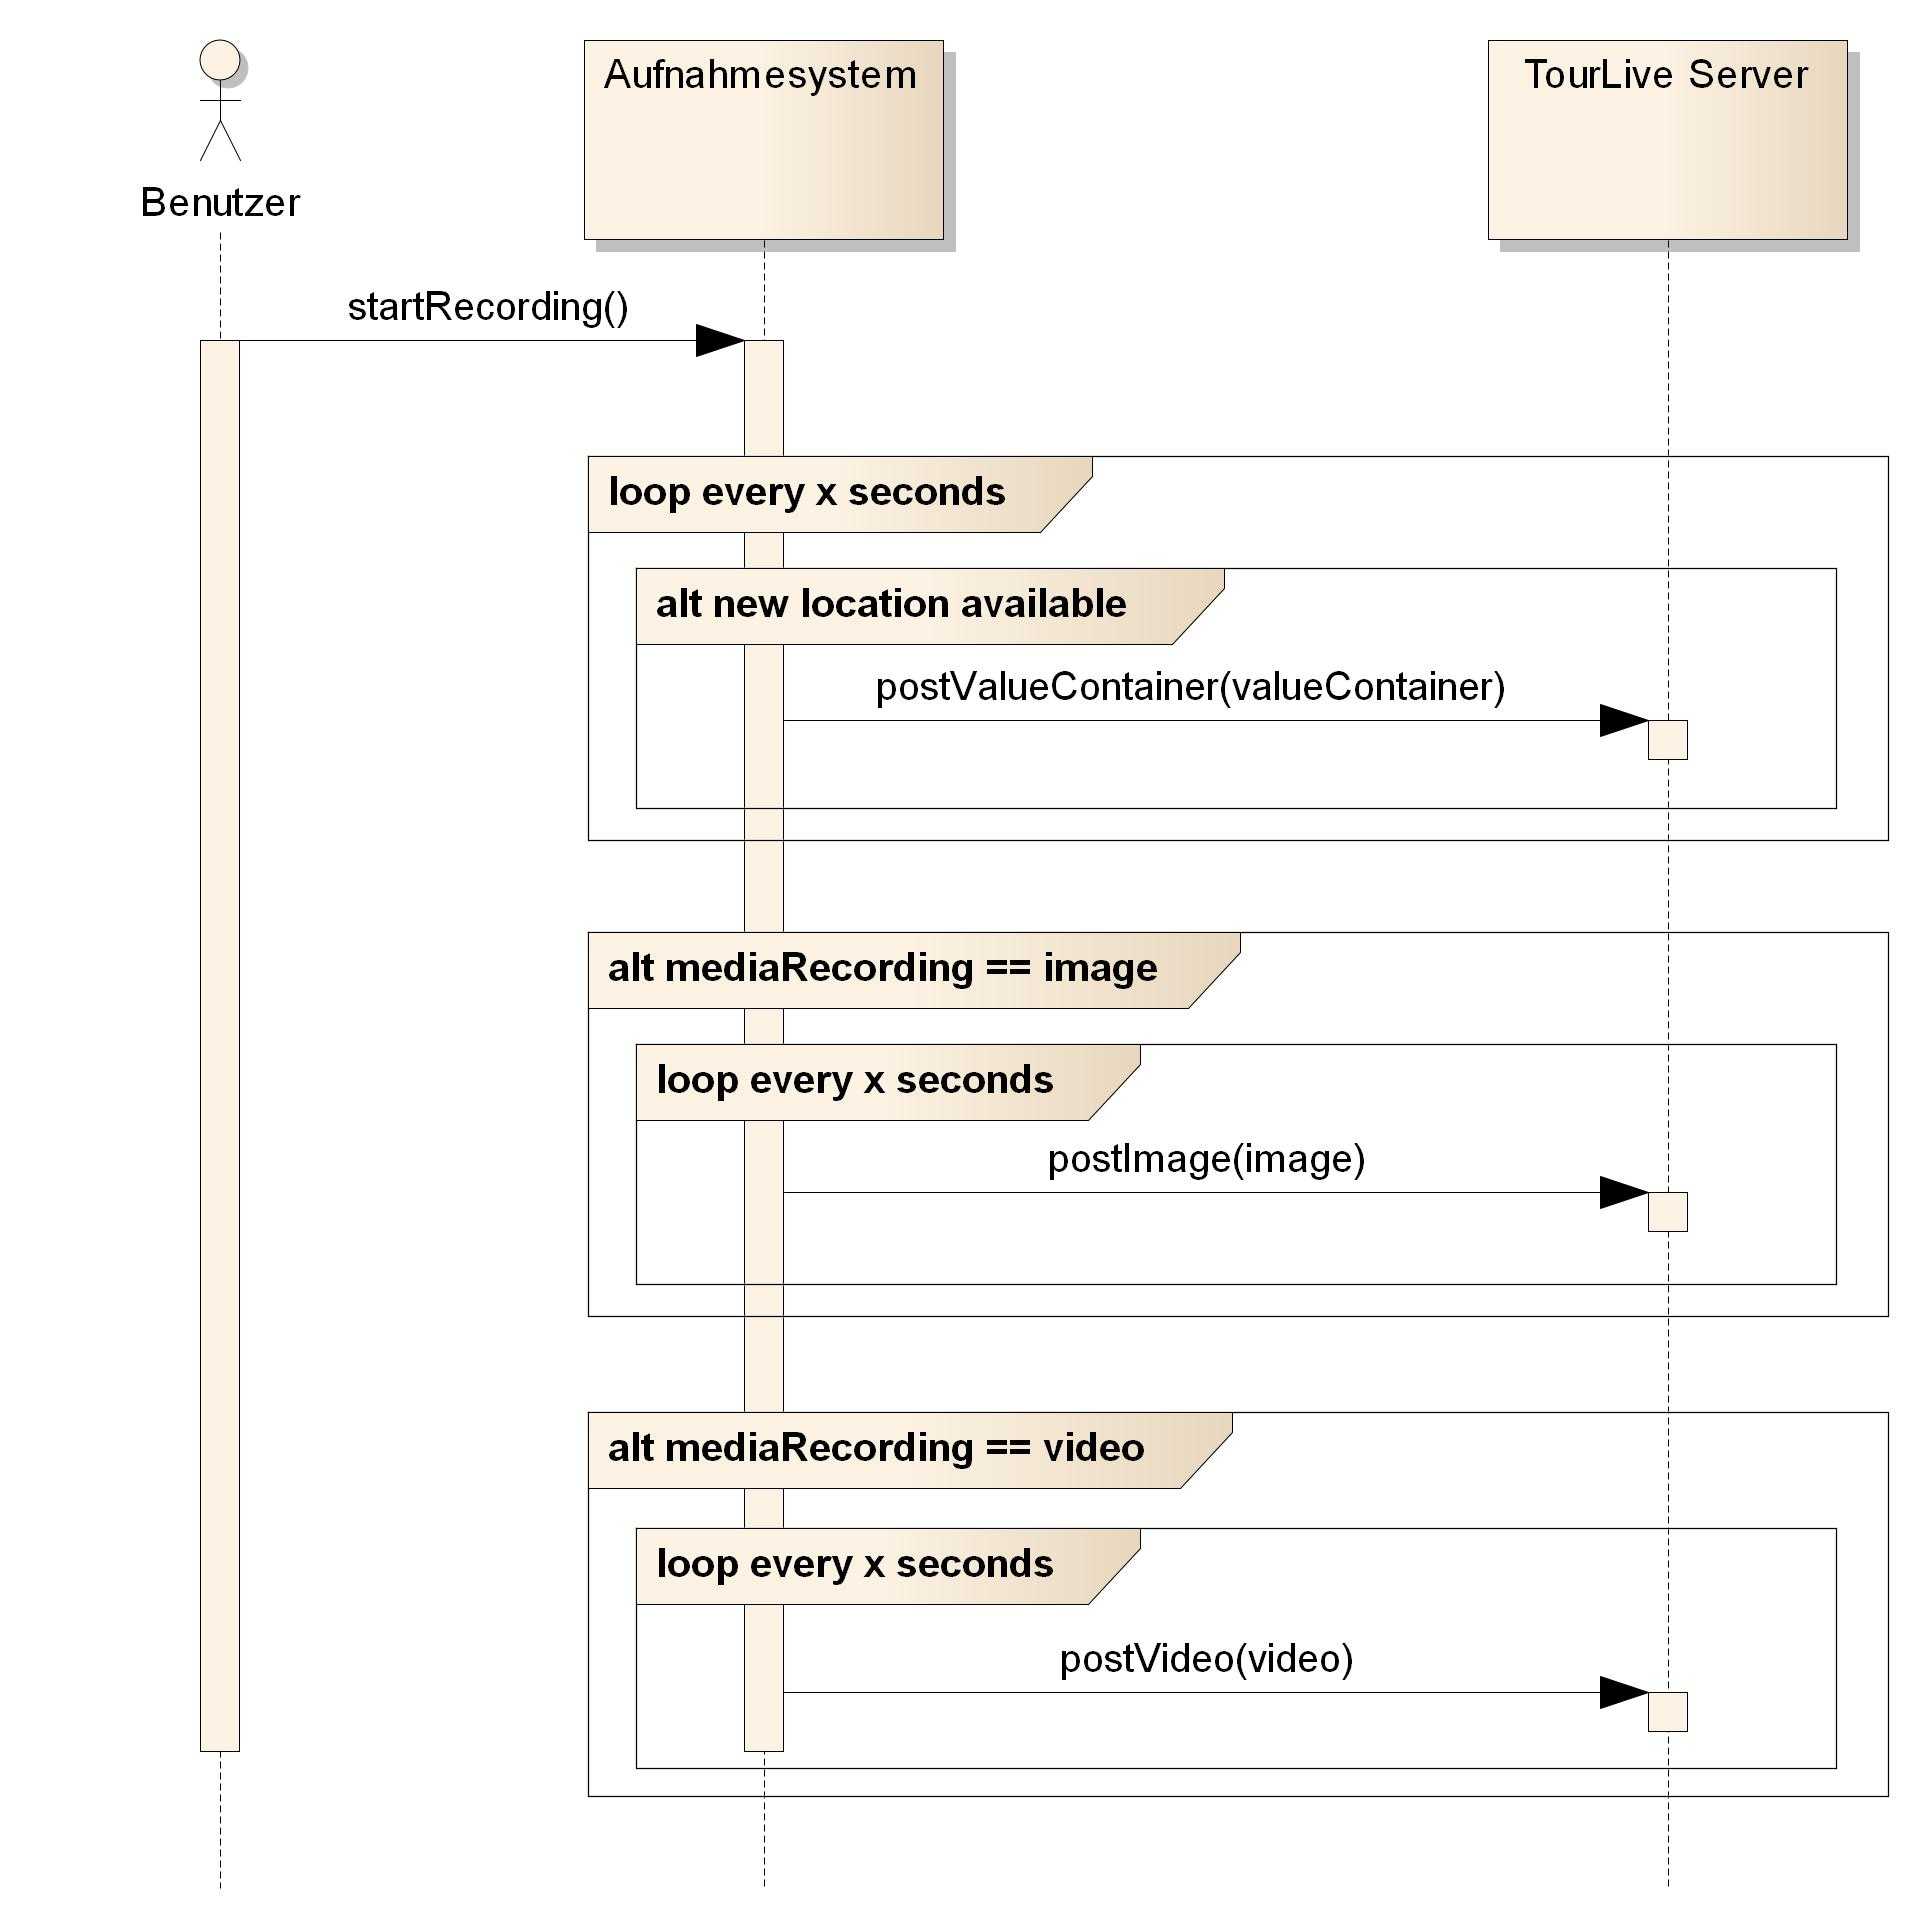
\includegraphics[width=150mm]{images/android/recording.jpg}
	\caption{Aufnahmesystem Aufnahme}
\end{figure}

\subsection{Algorithmen}
Das Aufnahmesystem enthält einige Algorithmen zur Berechnung von Distanzen, Steigungen und Zeit. Diese werden in folgendem Unterkapitel kurz beschrieben. Damit eine Berechnung durchgeführt werden kann wird ein \textit{StageInfo}-Objekt vorausgesetzt der beschreibt in welchem Rennen beziehungsweise in welcher Etappe sich das Aufnahmegerät aktuell befindet.
\\

\subsubsection{Berechnung der Renndauer}
Die Renndauer ist in der TourLive Applikation im Tab Etappe (eng. Stage) zu finden und beschreibt die Renndauer seit dem offiziellen Etappenstart gemäss \textit{StageInfo}. Die Berechnung der Renndauer erfolgt durch eine einfache Subtraktion.


\begin{algorithm}[H]
\begin{algorithmic}[1]
\vspace{5pt}
\If {$StageInfo \neq null$}
     \State \Return $now$ - $StageInfo.StageStartTime$;
\Else
     \State \Return $0$;
\EndIf
\end{algorithmic}
\caption{Berechnung der Renndauer}
\end{algorithm}


Die Renndauer wird bei der Erstellung eines \textit{ValueContainers} im assoziierten \textit{StageData} im Attribut \textit{stageTime} gespeichert.

\subsubsection{Berechnung der überwundenen Höhenmeter}
Die überwundenen Höhenmeter repräsentieren das Total der positiv überwundenen Höhenmeter während einer Etappe. Der Wert wird in der TourLive Applikation im Tab Etappe (eng. Stage) angezeigt. Die Berechnung erfolgt nach folgendem Algorithmus.

\begin{algorithm}[H]
\begin{algorithmic}[1]
\vspace{5pt}
\State $Altitude \gets 0$;
\State $CurrentAltitude \gets null$;
\State $NextAltitude \gets null$;
\ForAll{$ValueContainers$ since $StageInfo.StageStartTime$}
\If {$NextAltitude \neq null$}
\State $CurrentAltitude \gets ValueContainer.Altitude$;
\If {$CurrentAltitude \leq NextAltitude$}
     \State $Altitude\gets Altitude + (NextAltitude - CurrentAltitude)$
\EndIf
\Else
\State $NextAltitude \gets ValueContainer.Altitude$;
\EndIf
\EndFor
\end{algorithmic}
\caption{Berechnung der überwundenen Höhenmeter}
\end{algorithm}


Die überwundenen Höhenmeter werden bei der Erstellung eines \textit{ValueContainers} im assoziierten \textit{StageData} im Attribut \textit{stageUpAltitude} gespeichert.

\subsubsection{Berechnung der Steigung}
Die Angabe zur Steigung beziehen sich auf die letzten 100m Horizontaldistanz. Die Steigung wird im Tab Etappe (eng. Stage) angezeigt und bei der Erstellung eines \textit{ValueContainers} im assoziierten \textit{StageData} als Attribut \textit{incline} gespeichert. Die Berechnung erfolgt nach folgendem Algorithmus.


\begin{algorithm}[H]
\begin{algorithmic}[1]
\vspace{5pt}
\State $Altitude \gets 0$;
\State $Distance \gets 0$;
\State $LastAltitude \gets null$;
\State $LastDistance \gets null$;
\ForAll{$ValueContainers.Reverse$}
\If {$valueContainer$ is in $currentStage$}
\State $CurrAltitude \gets ValueContainer.Altitude$;
\State $CurrDistance \gets ValueContainer.Distance$;
\If {$LastAltitude \neq null$ \textbf{and} $LastDistance \neq null$ }
\State $Altitude \gets Altitude + (LastAltitude - CurrAltitude)$;
\State $Distance \gets Distance + (LastDistance - CurrDistance)$;
\EndIf
\State $LastAltitude \gets CurrAltitude$;
\State $LastDistance \gets CurrDistance$;
\If {$Distance \geq 100$}
\State BREAK;
\EndIf
\Else
\State BREAK;
\EndIf
\EndFor
\State $Incline \gets altitude/distance$;
\State \Return $arctan(incline.toDegrees)$;
\end{algorithmic}
\caption{Berechnung der Steigung}
\end{algorithm}

\subsubsection{Allgemeine Algorithmen zur Vermeidung von Berechnungsfehlern}
Die Erstellung eines ValueContainers erfolgt sobald das Aufnahmegerät eine neue Position meldet. Es kann vorkommen, dass die GPS-API von Android fehlerhafte Positionsdaten liefert. Aus diesem Grund werden erstellte ValueContainer auf ihre Datenkonsistenz überprüft und gegebenenfalls wieder verworfen. Der ValueContainer wird nach folgenden Kriterien überprüft:
\begin{itemize} [noitemsep,topsep=0pt]
\item longitude != 0
\item latitude != 0
\item accuracy < 100m
\item returned location from GPS\_PROVIDER != null
\end{itemize}

\subsection{TourLive Recovery Service}
Die Notfallwiederherstellung wie sie in den Anforderungen ans Aufnahmesystem formuliert ist, wurde aus Gründen der Zuverlässigkeit und Stabilität als separate Android Applikation (\textit{TourLiveRecoveryService.apk}) realisiert. Der TourLiveRecoveryService startet beim Gerätestart automatisch und besteht aus zwei Komponenten. Der SmsReceiver scannt einkommende SMS nach dem Stichwort \textit{RESTART} und sendet, falls dieses Stichwort gefunden wurde, eine Nachricht (Intent) an die TourLive Applikation um diese nach einem Absturz erneut zu starten. 

\chapter{Schnittstellen}

Das Aufnahmesystem kommuniziert sowohl mit dem TourLive Server als auch mit dem Device Management Server in beide Richtungen. In diesem Kapitel werden die Schnittstellen zwischen Aufnahmesystem, TourLive Server sowie Device Management Server und die öffentliche Schnittstelle erläutert. Die folgende Graphik gibt einen Überblick über alle Schnittstellen.

\begin{figure}[H]
	\centering
	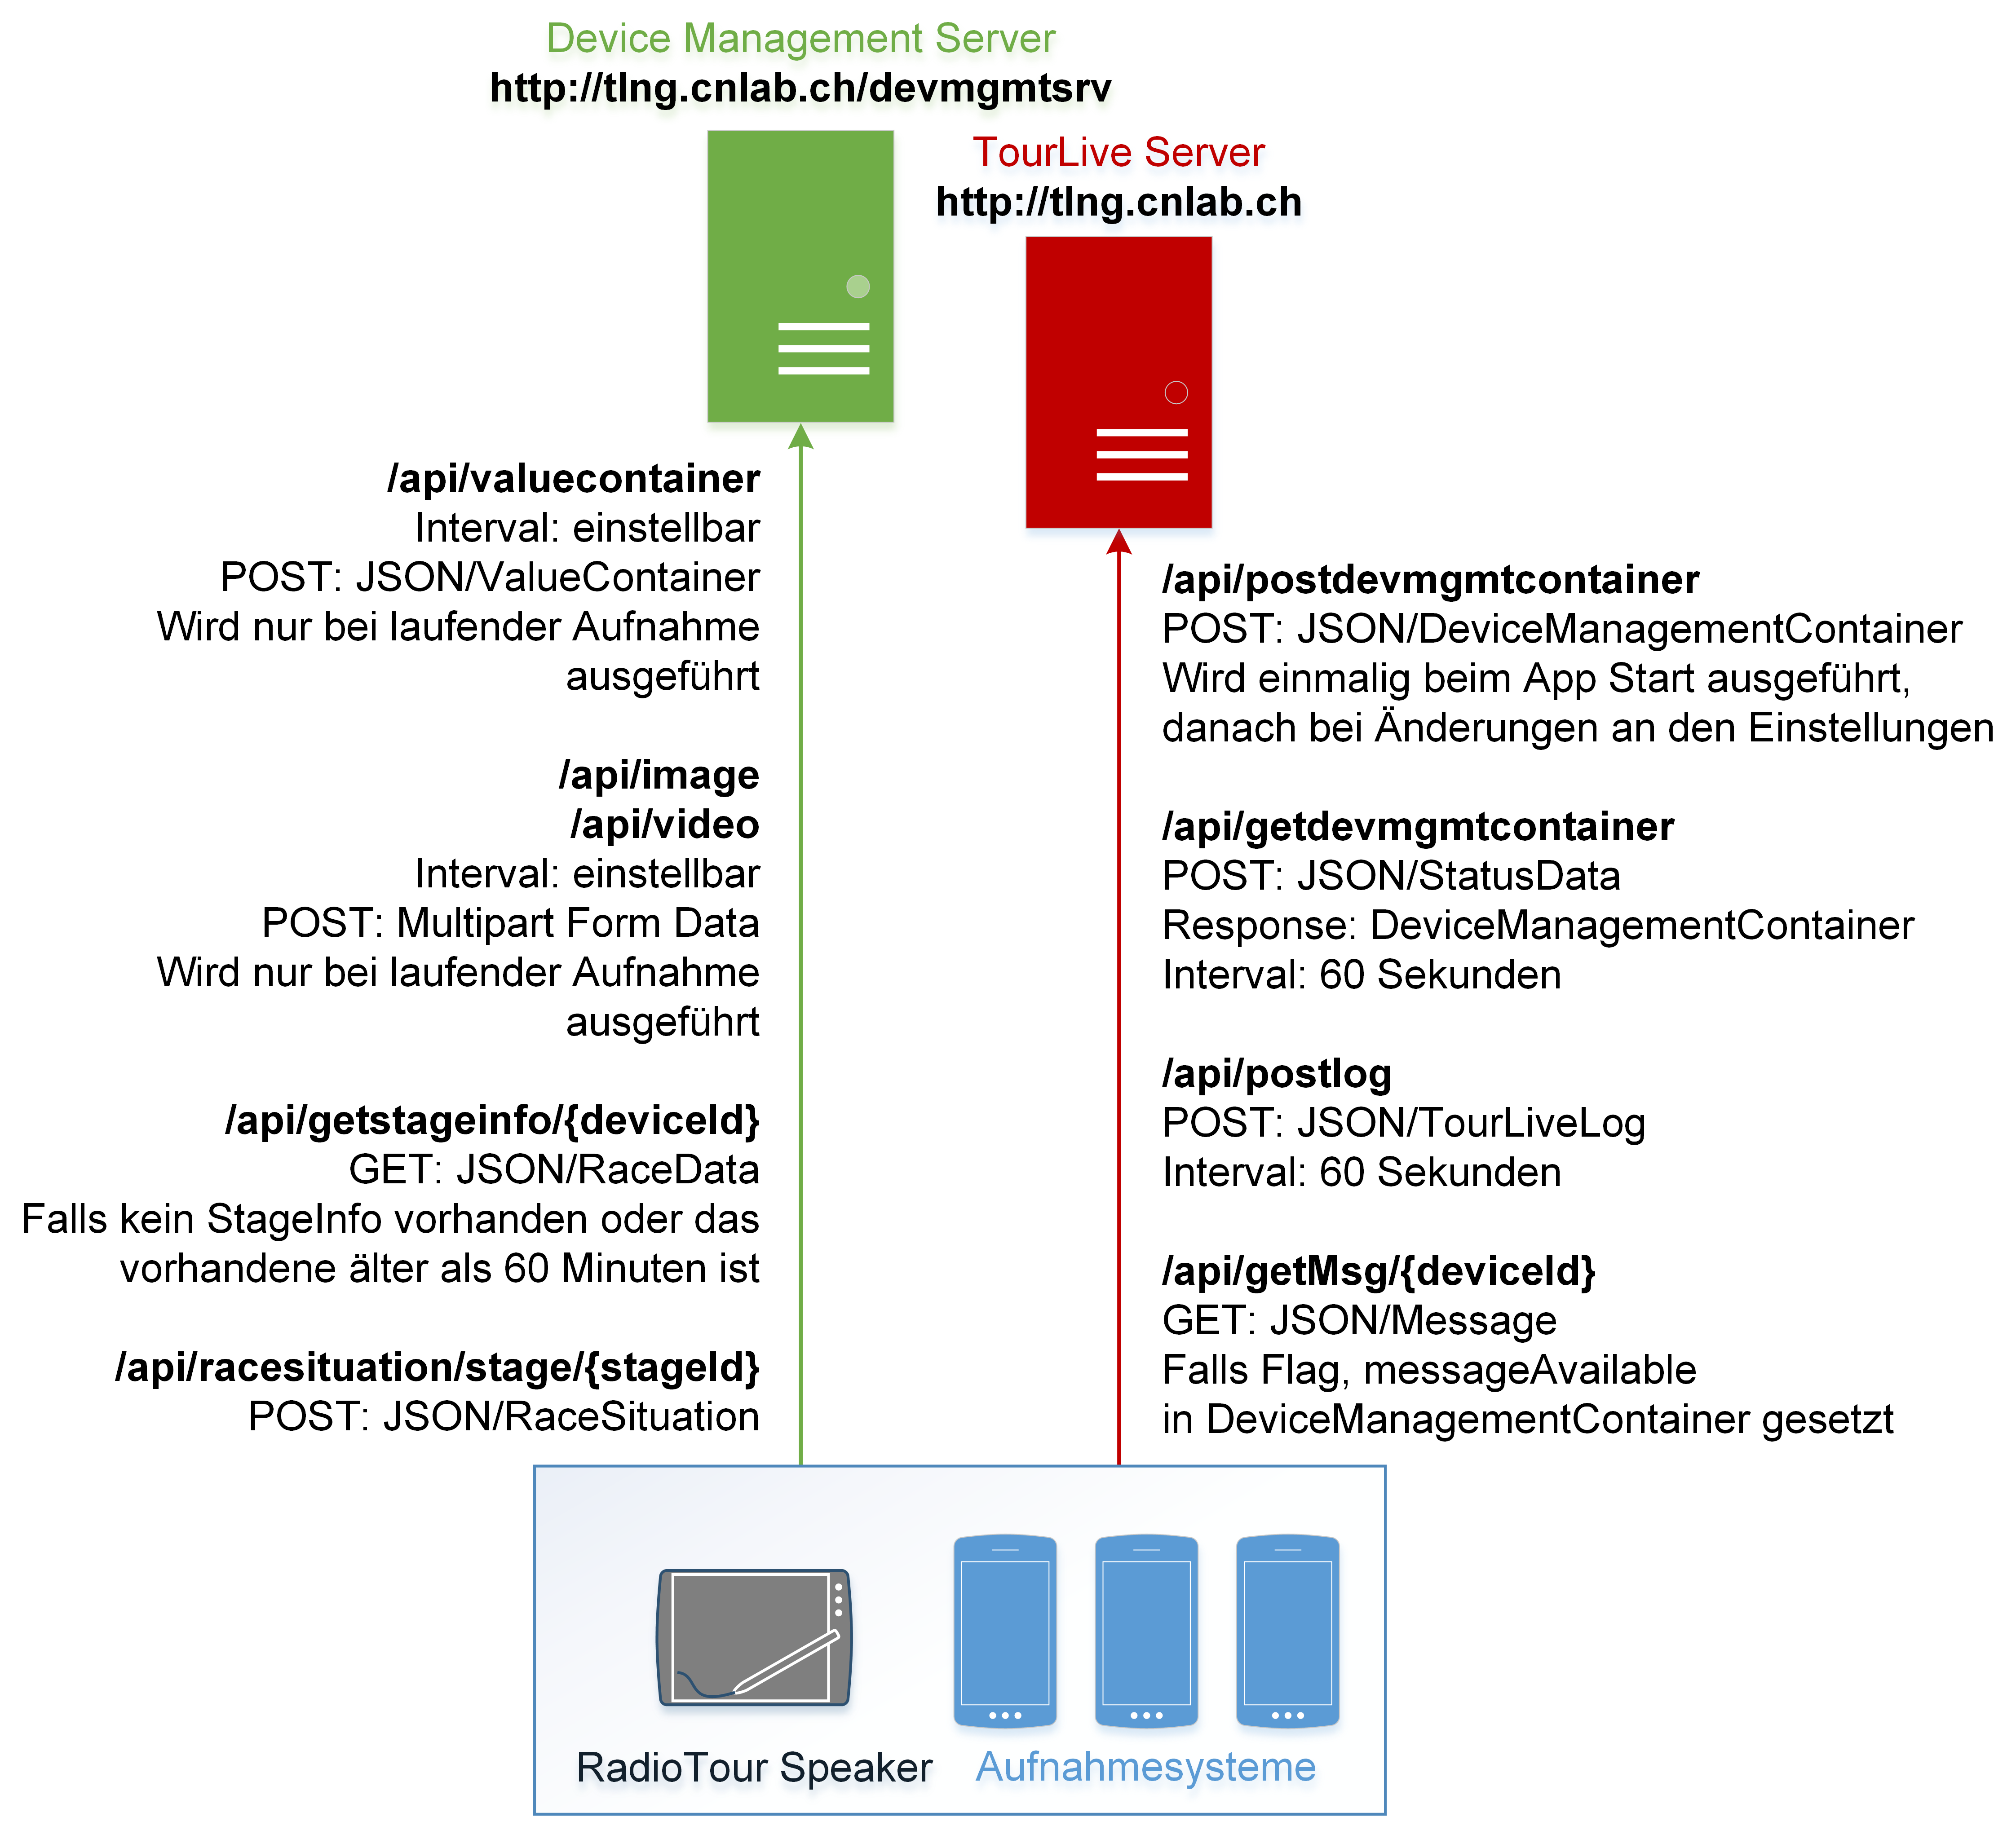
\includegraphics[width=130mm]{images/uebersicht_schnittstelle.png}
	\caption{Übersicht Schnittstellen}
\end{figure}

\section{TourLive Interne Schnittstelle}
\label{sec:tourliveserverapi}
Die Aufnahmegeräte liefern an dieser Stelle die ValueContainer, Bilder und Videos dem TourLive Server, dies wird als die interne Schnittstelle (\textit{\gls{api}}) bezeichnet. Die benötigten Felder sind jeweils im Bereich \textit{Request} erkennbar.

\subsection{ValueContainer posten}
\begin{longtable}{ p{2.5cm} p{3.5cm} p{6cm}}
	\textbf{URL:} & \multicolumn{2}{p{10cm}}{/api/valuecontainer} \\
	\textbf{Request:} & Method: & POST \\
		& Content-Type: & application/json \\
		& Body: & JSON-String 'ValueContainer'\\
	\textbf{Response:} & Header: & HTTP/1.1 200 OK \\
		& Body: & <empty> \\
	\textbf{Zeitpunkt:} & \multicolumn{2}{p{10cm}}{Bei laufender Aufnahme} \\ 
	\textbf{Interval:} & \multicolumn{2}{p{10cm}}{einstellbar} \\ 
	\caption{Schnittstelle ValueContainer}
\end{longtable}

\subsubsection{ValueContainer JSON}
\begin{figure}[H]
	\centering
	\lstinputlisting[language=json]{jsonfiles/valueContainer.json}
	\caption{ValueContainer JSON}
	\label{fig:valuecontainer}
\end{figure}

\subsection{Image posten}
\begin{longtable}{ p{2.5cm} p{3.5cm} p{6cm}}
	\textbf{URL:} & \multicolumn{2}{p{10cm}}{/api/image} \\
	\textbf{Request:} & Method: & POST \\
		& Content-Type: & multipart/form-data [3 Boundaries] \\
		& Body-Boundary 1: & text/plain (timestamp) \\
		& Body-Boundary 2: & text/plain (deviceId) \\
		& Body-Boundary 3: & application/octet-stream (Bild) \\
	\textbf{Response:} & Header: & HTTP/1.1 200 OK \\
		& Body: & <empty> \\
	\textbf{Zeitpunkt:} & \multicolumn{2}{p{10cm}}{Bei laufender Aufnahme, falls Image aktiviert ist} \\ 
	\textbf{Interval:} & \multicolumn{2}{p{10cm}}{einstellbar}
\end{longtable}

\subsection{Video posten}
\begin{longtable}{ p{2.5cm} p{3.5cm} p{6cm}}
	\textbf{URL:} & \multicolumn{2}{p{10cm}}{/api/video} \\
	\textbf{Request:} & Method: & POST \\
		& Content-Type: & multipart/form-data [3 Boundaries] \\
		& Body-Boundary 1: & text/plain (timestamp) \\
		& Body-Boundary 2: & text/plain (deviceId) \\
		& Body-Boundary 3: & application/octet-stream (Video) \\
	\textbf{Response:} & Header: & HTTP/1.1 200 OK \\
		& Body: & <empty> \\
	\textbf{Zeitpunkt:} & \multicolumn{2}{p{10cm}}{Bei laufender Aufnahme, falls der Videostream aktiviert ist} \\ 
	\textbf{Interval:} & \multicolumn{2}{p{10cm}}{einstellbar} 
\end{longtable}

\subsection{RaceSituation posten}
\begin{longtable}{ p{2.5cm} p{3.5cm} p{6cm}}
	\textbf{URL:} & \multicolumn{2}{p{10cm}}{/api/racesituation/stage/\{stageId\}} \\
	\textbf{Request:} & Method: & POST \\
		& Body: & JSON-String 'RaceSituation'\\	
	\textbf{Response:} & Header: & HTTP/1.1 200 OK \\
		& Body: & <empty> \\	
	\textbf{Bemerkung:} & \multicolumn{2}{p{10cm}}{Der RadioTourSpeaker sendet (unabhängig von den TourLive Aufnahmegeräten) periodisch die Rennsituation an den Server}
\end{longtable}

\subsubsection{RaceSituation JSON}
Der TourLive Server erwartet das folgende JSON für die Darstellung der Rennsituation.
\begin{figure}[H]
	\centering
	\lstinputlisting[language=json]{jsonfiles/raceSituation.json}
	\caption{RaceSituation JSON}
\end{figure}


\subsection{StageInfo abfragen}
\begin{longtable}{ p{2.5cm} p{3.5cm} p{6cm}}
	\textbf{URL:} & \multicolumn{2}{p{10cm}}{/api/getstageinfo/\{deviceId\}} \\
	\textbf{Request:} & Method: & GET \\
		& Body: & <empty>\\	
	\textbf{Response:} & Header: & HTTP/1.1 200 OK \\
		& Content-Type: & application/json \\
		& Body: & Custom JSON-String \\	
	\textbf{Bemerkung:} & \multicolumn{2}{p{10cm}}{Im Body der Response wird eine eigens kreierte HashMap ausgeliefert, darin sind aktuelle Etappeninformationen für das angegebene Gerät. Diese Informationen werden für den Rennbegleiter auf dem Gerät dargestellt} \\ [1ex] 
\caption{Schnittstellen StageInfo}
\end{longtable}

\subsection{StageInfo JSON}
\begin{figure}[H]
	\centering
	\lstinputlisting[language=json]{jsonfiles/stageInfo.json}
	\caption{StageInfo JSON}
\end{figure}


\section{TourLive Public API}
\label{sec:tourlivepublicapi}
Die Renn- und Etappeninformationen stehen für Drittentwickler zur Verfügung. Zu jeder Etappe können zusätzlich die ValueContainer und Bilddaten abgefragt werden. Diese Schnittstelle wird mit \textit{Publc API} bezeichnet.

\subsection{Etappen abfragen}
\begin{longtable}{ p{2.5cm} p{3.5cm} p{6cm}}
	\textbf{URL:} & \multicolumn{2}{l}{/public/stages} \\
	\textbf{Request:} & Method: & GET \\
		& Body: & <empty>\\
	\textbf{Response:} &  Header: & HTTP/1.1 200 OK \\
		& Content-Type: & application/json \\
		& Body: & JSON-Array 'Stages'\\
	\textbf{Bemerkung:} & \multicolumn{2}{p{10cm}}{Alle sichtbaren Etappen} 
\end{longtable}
\subsubsection{Etappen JSON}
\begin{figure}[H]
	\centering
	\lstinputlisting[language=json]{jsonfiles/stages.json}
	\caption{Etappen JSON}
\end{figure}

\subsection{ValueContainer abfragen}
\begin{longtable}{ p{2.5cm} p{3.5cm} p{6cm}}
	\textbf{URL:} & \multicolumn{2}{l}{/public/stage/\{stageId\}/valuecontainer} \\
	\textbf{Request:} & Method: & GET \\
		& Body: & <empty>\\
	\textbf{Response:} &  Header: & HTTP/1.1 200 OK \\
		& Content-Type: & application/json \\
		& Body: & JSON-Array 'ValueContainers'\\
	\textbf{Bemerkung:} & \multicolumn{2}{p{10cm}}{Alle ValueContainers einer Etappe}
\end{longtable}

\subsection{ImageData abfragen}
\begin{longtable}{ p{2.5cm} p{3.5cm} p{6cm}}
	\textbf{URL:} & \multicolumn{2}{l}{/public/stage/\{stageId\}/imagedata} \\
	\textbf{Request:} & Method: & GET \\
		& Body: & <empty>\\
	\textbf{Response:} &  Header: & HTTP/1.1 200 OK \\
		& Content-Type: & application/json \\
		& Body: & JSON-Array 'ImageData'\\
	\textbf{Bemerkung:} & \multicolumn{2}{p{10cm}}{Alle ImageData Objekte zu dieser Etappe, nicht aber die eigentlichen Bilder. Die Bilder können aber mit dem Feld \textit{imageLocation} entweder direkt verlinkt oder heruntergeladen werden}
\end{longtable}

\subsubsection{ImageData JSON}
\begin{figure}[H]
	\centering
	\lstinputlisting[language=json]{jsonfiles/imageData.json}
	\caption{ImageData JSON}
\end{figure}

\subsection{VideoData abfragen}	
\begin{longtable}{ p{2.5cm} p{3.5cm} p{6cm}}
	\textbf{URL:} & \multicolumn{2}{l}{/public/stage/\{stageId\}/videodata} \\
	\textbf{Request:} & Method: & GET \\
		& Body: & <empty>\\
	\textbf{Response:} &  Header: & HTTP/1.1 200 OK \\
		& Content-Type: & application/json \\
		& Body: & JSON-Array 'VideoData'\\
	\textbf{Bemerkung:} & \multicolumn{2}{p{10cm}}{Alle VideoData Objekte zu dieser Etappe, nicht aber die eigentlichen Videosequenzen. Die Videos können aber mit dem Feld \textit{videoLocation} entweder direkt verlinkt oder heruntergeladen werden}
\end{longtable}

\subsection{MarchTableItem abfragen}
\begin{longtable}{ p{2.5cm} p{3.5cm} p{6cm}}
	\textbf{URL:} & \multicolumn{2}{l}{/public/stage/\{stageId\}/marchtableitem} \\
	\textbf{Request:} & Method: & GET \\
		& Body: & <empty>\\
	\textbf{Response:} &  Header: & HTTP/1.1 200 OK \\
		& Content-Type: & application/json \\
		& Body: & JSON-Array 'MarchTableItem'\\
	\textbf{Bemerkung:} & \multicolumn{2}{p{10cm}}{Die Marschtabelle ist aufgeteilt in Einheiten. Jede Reihe bedeutet eine Einheit. Pro Etappe können alle Marschtabelleneinheiten abgerufen werden.}
\end{longtable}

\subsubsection{MarchTableItem abfragen}
\begin{figure}[H]
	\centering
	\lstinputlisting[language=json]{jsonfiles/marchTableItems.json}
	\caption{MarchTableItem JSON}
\end{figure}

\subsection{Riders abfragen}
\begin{longtable}{ p{2.5cm} p{3.5cm} p{6cm}}	
	\textbf{URL:} & \multicolumn{2}{l}{/public/stage/\{stageId\}/riders} \\
	\textbf{Request:} & Method: & GET \\
		& Body: & <empty>\\
	\textbf{Response:} &  Header: & HTTP/1.1 200 OK \\
		& Content-Type: & application/json \\
		& Body: & JSON-Array 'Riders'\\
	\textbf{Bemerkung:} & \multicolumn{2}{p{10cm}}{Sämtliche Fahrer, welche dieser Etappe zugeordnet sind} \\ [1ex] 
\caption{TourLive Public API}
\end{longtable}

\subsubsection{Riders JSON}
\begin{figure}[H]
	\centering
	\lstinputlisting[language=json]{jsonfiles/riders.json}
	\caption{Riders JSON}
\end{figure}

\section{Device Management Portal Schnittstelle}

\subsection{Einstellungen posten}
Sobald die Einstellungen in der App geändert werden, müssen sie über diese Schnittstelle an den Server gesendet werden.

{\renewcommand{\arraystretch}{1}
    \begin{longtable}{ p{2.5cm} p{3.5cm} p{6cm}}
	\textbf{URL:} & \multicolumn{2}{l}{/devmgmtsrv/api/postdevmgmtsrv} \\
	\textbf{Request:} & Method: & POST \\
		& Content-Type: & application/json \\
		& Body: & JSON-String 'DeviceManagementContainer'\\
	\textbf{Response:} &  Header: & HTTP/1.1 200 OK \\
		& Body: & <empty>	\\
	\textbf{Eigenschaft:} & \multicolumn{2}{p{10cm}}{Wird einmalig beim App Start ausgeführt sowie bei lokalen Änderungen in den Einstellungen} \\
	\textbf{Interval:} & \multicolumn{2}{p{10cm}}{unregelmässig} \\
	
\caption{Schnittstelle Einstellungen}
\end{longtable}}

\subsubsection{Einstellungen JSON}
\begin{figure}[H]
	\centering
	\lstinputlisting[language=json]{jsonfiles/settings.json}
	\caption{Einstellungen JSON}
\end{figure}

\subsection{Status posten und Einstellungen erhalten}

Um den aktuellen Status des Aufnahmesystems dem Server mitzuteilen kann diese Methode aufgerufen werden. Als Antwort erhält man die im Moment aktuellen Einstellungen.

{\renewcommand{\arraystretch}{1}
    \begin{longtable}{ p{2.5cm} p{3.5cm} p{6cm}} 
	\textbf{URL:} & \multicolumn{2}{l}{/devmgmtsrv/api/getdevmgmtsrv} \\
	\textbf{Request:} & Content-Type: & application/json \\
		& Method: & POST \\
		& Body: & JSON-String 'StatusData' \\
	\textbf{Response:} & Method: & POST \\
		& Content-Type: & application/json \\
		& Body: & JSON-String 'DeviceManagementContainer' \\
	\textbf{Eigenschaft:} & \multicolumn{2}{p{10cm}}{Wird regelmässig als Service ausgeführt.} \\ 
	\textbf{Interval:} & \multicolumn{2}{p{10cm}}{regelmässig - alle 60 Sekunden} \\
	
\caption{Schnittstelle Status}
\end{longtable}	}
\subsubsection{Status JSON}

Das JSON eines Status Posts sieht folgendermassen aus:

\begin{figure}[H]
	\centering
	\lstinputlisting[language=json]{jsonfiles/status.json}
	\caption{Status JSON}
\end{figure}


\subsection{Log posten}

Um neue Logeinträge dem Server zu übermitteln kann diese Methode benutzt werden.

{\renewcommand{\arraystretch}{1}
    \begin{longtable}{ p{2.5cm} p{3.5cm} p{6cm}}
	\textbf{URL:} & \multicolumn{2}{p{10cm}}{/devmgmtsrv/api/postlog} \\
	\textbf{Request:} & Method: & POST \\
		& Content-Type: & application/json \\
		& Body: & JSON-String 'TourLiveLog' \\
	\textbf{Response:} &  Header: & HTTP/1.1 200 OK \\
		& Body: & <empty>	\\
	\textbf{Eigenschaft:} &  \multicolumn{2}{p{10cm}}{Wird regelmässig als Service ausgeführt.}\\ 
	\textbf{Interval:} &  \multicolumn{2}{p{10cm}}{regelmässig - alle 60 Sekunden}\\
	
\caption{Schnittstelle Log}
\end{longtable}}

\subsubsection{Log JSON}

Das JSON eines Log Posts sieht folgendermassen aus:

\begin{figure}[H]
	\centering
	\lstinputlisting[language=json]{jsonfiles/log.json}
	\caption{Log JSON}
\end{figure}

\subsection{Nachricht abholen}

Sofern eine neue Nachricht für das Gerät vorhanden ist kann sie über diese Methoden abgeholt werden.

{\renewcommand{\arraystretch}{1}
    \begin{longtable}{ p{2.5cm} p{3.5cm} p{6cm}}

	\textbf{URL:} & \multicolumn{2}{p{10cm}}{/devmgmtsrv/api/getMsg/\{deviceId\}} \\
	\textbf{Request:} & Method: & GET \\
		& Body: & <empty> \\
	\textbf{Response:} & Method: & POST \\
		& Content-Type: & application/json \\
		& Body: & JSON-String 'Message' \\
	\textbf{Eigenschaft:} & \multicolumn{2}{p{10cm}}{ Wenn das 'messageAvailable'-Flag gesetzt ist in einem empfangenen DeviceManagementContainer.} \\
	\textbf{Interval:} & \multicolumn{2}{p{10cm}}{unregelmässig}\\
	
\caption{Schnittstelle Nachricht abholen}
\end{longtable} }

\subsubsection{Nachrichten JSON}
Das JSON für die Nachrichten ist das folgende:
\begin{figure}[H]
	\centering
	\lstinputlisting[language=json]{jsonfiles/message.json}
	\caption{Nachrichten JSON}
\end{figure}



\chapter{Ergebnise und Schlussfolgerungen}

Lorem ipsum dolor sit amet, consectetur adipiscing elit. Sed gravida mollis placerat. Sed congue iaculis massa vitae dapibus. Fusce sed felis lorem. Suspendisse purus diam, sollicitudin vitae imperdiet ac, placerat eu metus. In luctus, metus vel dictum hendrerit, diam lacus cursus enim, eu porta augue lacus non metus. Pellentesque habitant morbi tristique senectus et netus et malesuada fames ac turpis egestas. Nullam nec orci eget metus pulvinar sagittis. Vestibulum ante ipsum primis in faucibus orci luctus et ultrices posuere cubilia Curae; Sed turpis lorem, aliquet eu ornare non, viverra ac urna.

\section{Endprodukt}

Praesent libero lectus, ultrices eget pharetra sed, sollicitudin et est. Pellentesque quis urna eget lorem sodales venenatis eget nec quam. In sagittis aliquam auctor. Phasellus vitae ipsum purus, sit amet imperdiet nunc. Pellentesque habitant morbi tristique senectus et netus et malesuada fames ac turpis egestas. Ut malesuada nibh ut lectus scelerisque sed iaculis lectus varius. Nulla blandit turpis tortor. Nulla facilisi. Cum sociis natoque penatibus et magnis dis parturient montes, nascetur ridiculus mus. Nam leo ante, porta vel scelerisque at, volutpat eu sapien. Aliquam viverra adipiscing sapien et porta. Sed quis diam ut sem tincidunt consectetur varius non dolor. Fusce fermentum, quam vitae suscipit euismod, leo erat malesuada ante, ac consequat est lacus eget enim. Proin lacinia justo et est vehicula adipiscing rhoncus lacus mollis.

\section{Ausblick}

Lorem ipsum dolor sit amet, consectetur adipiscing elit. Sed gravida mollis placerat. Sed congue iaculis massa vitae dapibus. Fusce sed felis lorem. Suspendisse purus diam, sollicitudin vitae imperdiet ac, placerat eu metus. In luctus, metus vel dictum hendrerit, diam lacus cursus enim, eu porta augue lacus non metus. Pellentesque habitant morbi tristique senectus et netus et malesuada fames ac turpis egestas. Nullam nec orci eget metus pulvinar sagittis. Vestibulum ante ipsum primis in faucibus orci luctus et ultrices posuere cubilia Curae; Sed turpis lorem, aliquet eu ornare non, viverra ac urna.

% List of figures & glossary
%%%%%%%%%%%%%%%%%%%%%%%%%%%%
\listoffigures
\printglossary[style=altlist,title=Glossar]

% Bibliography
%%%%%%%%%%%%%%
\bibliographystyle {alpha}
\bibliography{index/bibliography}

% Anhang
%%%%%%%%%%%%%%%%%%
\chapter{Anhang}

Lorem ipsum dolor sit amet, consectetur adipiscing elit. Sed gravida mollis placerat. Sed congue iaculis massa vitae dapibus. Fusce sed felis lorem. Suspendisse purus diam, sollicitudin vitae imperdiet ac, placerat eu metus. In luctus, metus vel dictum hendrerit, diam lacus cursus enim, eu porta augue lacus non metus. Pellentesque habitant morbi tristique senectus et netus et malesuada fames ac turpis egestas. Nullam nec orci eget metus pulvinar sagittis. Vestibulum ante ipsum primis in faucibus orci luctus et ultrices posuere cubilia Curae; Sed turpis lorem, aliquet eu ornare non, viverra ac urna.

\section{Projektorganisation}

Praesent libero lectus, ultrices eget pharetra sed, sollicitudin et est. Pellentesque quis urna eget lorem sodales venenatis eget nec quam. In sagittis aliquam auctor. Phasellus vitae ipsum purus, sit amet imperdiet nunc. Pellentesque habitant morbi tristique senectus et netus et malesuada fames ac turpis egestas. Ut malesuada nibh ut lectus scelerisque sed iaculis lectus varius. Nulla blandit turpis tortor. Nulla facilisi. Cum sociis natoque penatibus et magnis dis parturient montes, nascetur ridiculus mus. Nam leo ante, porta vel scelerisque at, volutpat eu sapien. Aliquam viverra adipiscing sapien et porta. Sed quis diam ut sem tincidunt consectetur varius non dolor. Fusce fermentum, quam vitae suscipit euismod, leo erat malesuada ante, ac consequat est lacus eget enim. Proin lacinia justo et est vehicula adipiscing rhoncus lacus mollis.

\section{Persönliche Berichte}

\subsection{Florian Bentele}
Praesent libero lectus, ultrices eget pharetra sed, sollicitudin et est. Pellentesque quis urna eget lorem sodales venenatis eget nec quam. In sagittis aliquam auctor. Phasellus vitae ipsum purus, sit amet imperdiet nunc. 

\subsection{Patrizia Heer}
Praesent libero lectus, ultrices eget pharetra sed, sollicitudin et est. Pellentesque quis urna eget lorem sodales venenatis eget nec quam. In sagittis aliquam auctor. Phasellus vitae ipsum purus, sit amet imperdiet nunc. 

\subsection{Simon Stäheli}
Praesent libero lectus, ultrices eget pharetra sed, sollicitudin et est. Pellentesque quis urna eget lorem sodales venenatis eget nec quam. In sagittis aliquam auctor. Phasellus vitae ipsum purus, sit amet imperdiet nunc.

\section{Designentscheid}
Warum JSON warum Restful? Praesent libero lectus, ultrices eget pharetra sed, sollicitudin et est. Pellentesque quis urna eget lorem sodales venenatis eget nec quam. In sagittis aliquam auctor. Phasellus vitae ipsum purus, sit amet imperdiet nunc. 

\section{Werzeuge und Entwicklungsumgebung}
Praesent libero lectus, ultrices eget pharetra sed, sollicitudin et est. Pellentesque quis urna eget lorem sodales venenatis eget nec quam. In sagittis aliquam auctor. Phasellus vitae ipsum purus, sit amet imperdiet nunc. 

\section{Plakat}
<<hier kommt das Plakat>>

\section{Developer Guide}
Installationsanleitung für die weitere Entwicklung.
Praesent libero lectus, ultrices eget pharetra sed, sollicitudin et est. Pellentesque quis urna eget lorem sodales venenatis eget nec quam. In sagittis aliquam auctor. Phasellus vitae ipsum purus, sit amet imperdiet nunc. 

\section{Zugänge}
Die Coderepositories sind auf Github öffentlich zugänglich. Zugang zum Server... Praesent libero lectus, ultrices eget pharetra sed, sollicitudin et est. Pellentesque quis urna eget lorem sodales venenatis eget nec quam. In sagittis aliquam auctor. Phasellus vitae ipsum purus, sit amet imperdiet nunc. 

\section{Kontaktadressen}
Die Studierenden:\\
Simon Stäheli\\
Richterswil\\
sstaehel@hsr.ch\\

Patrizia Heer\\
Thundorf\\
pheer@hsr.ch\\

Florian Bentele\\
Teufener Strasse 113\\
9000 St. Gallen\\
+41 78 883 68 65\\
florian@bentele.me\\

Der betreuende Professor\\
Prof. Dr. Peter Heinzman, cnlab AG\\
Obere Bahnhofstrasse 32b\\
8640 Rapperswil\\
+41 79 243 04 61\\
peter.heinzmann@cnlab.ch\\

Der Industriepartner\\
Lukas Frey, cnlab AG\\
Obere Bahnhofstrasse 32b\\
8640 Rapperswil\\
+41 55 214 33 44\\
lukas.frey@cnlab.ch

\section{Inhaltsverzeichnis der CD}
.\\
|-01Dokumente-cnlab\\
||Alte Logos\\
||logo.png\\
|-02Protokolle\\
|--01Protokoll.doc\\
|--02Protokoll.doc\\



\end{document}